\documentclass[oneside]{ZJUthesis}

% 该文档中首字符为“%”的均为注释行,不会在论文中出现

% 论文默认为双面模式,需单面模式请将第一行换为如下所示:
% \documentclass[oneside]{ZJUthesis}

% 取消目录中链接的颜色,方便打印
% 如需颜色,请将“false”改为“true”
\hypersetup{colorlinks=false}

%\usepackage[sectionbib]{chapterbib}

\begin{document}
%%%%%%%%%%%%%%%%%%%%%%%%%%%%%
%% 正文字体设定
%%%%%%%%%%%%%%%%%%%%%%%%%%%%%
\fangsong

%%%%%%%%%%%%%%%%%%%%%%%%%%%%%
%% 论文封面部分
%%%%%%%%%%%%%%%%%%%%%%%%%%%%%
% 中文封面内容

% 中图分类号
\classification{TM863}

% 单位代码
\serialnumber{10335}

% 密级,如需密级则将其前“%”去掉
%\SecretLevel{绝密}

% 学号
\PersonalID{127436}

\title{论文~LaTeX~版本快速指南}
% 如果标题一行写不下,就写成两行,在下面的命令里写第二行,不需要两行则注释掉
\titletl{第二版}
%\titletl{test}

%英文题目
\Etitle{Thesis LaTeX Fast Guide}
% 如果一行写不下,同中文题目设定,一行写不下则写两行,不需要就注释掉
\Etitletl{The Second Edition}

% 作者
\author{王东举}

\degree{某士}

% 导师
\supervisor{各类\hspace{1em} 网络文档}

% 合作导师,如果有的话,去掉注释,
%\cpsupervisor{某 \quad某某}

% 专业名称
\major{电气工程}

% 研究方向
\researchdm{我的方向}

% 所属学院
\institute{电气工程学院}

%论文提交日期
\submitdate{2015年4月8日}

% 答辨日期
\defenddate{2015年6月12日}
\defenddateE{June 12th, 2015}

% 生成封面
\makeCoverPage

%%%%%%%%%%%%%%%%%%%%%%%%%%%%%%
%% 中文题名页内容
%%%%%%%%%%%%%%%%%%%%%%%%%%%%%%
% 论文评阅人信息 注意两字名与三字名,两字职称与三字职称的写法,便于对齐
% 多余的名额直接注释掉即可,比如三个评阅人,把评阅人D,E注释掉即可
\reviewersA{丘处机\hspace{1.5em}真人\hspace{1.5em}登州滨都宫\hspace{1em}}
\reviewersB{葛\quad 洪\hspace{1.5em}方士\hspace{1.5em}罗浮山道观\hspace{1em}}
\reviewersC{寇谦之\hspace{1.5em}天师\hspace{1.5em}嵩山中岳道场}
\reviewersD{张三丰\hspace{1.5em}真君\hspace{1.5em}武当玉虚宫\hspace{1em}}
\reviewersE{孙玄清\hspace{1.5em}真人\hspace{1.5em}崂山明霞洞\hspace{1em}}

% 答辩委员会信息,如果某一个单位比较长,
% 请在其它较短后面补上{hspace{Xem}},X是比最长的单位名少几个字
% 如果实际人数少于6人,多余的注释掉即可
\chairman{唐三藏\hspace{1.5em}功佛\hspace{1.5em}洛阳大慈恩寺}
\commissionerA{惠\quad 能\hspace{1.5em}方丈\hspace{1.5em}曹溪宝林寺\hspace{1em}}
\commissionerB{智\quad 顗\hspace{1.5em}方丈\hspace{1.5em}天台山国清寺}
\commissionerC{法\quad 藏\quad 大和尚\quad 洛阳佛授记寺}
\commissionerD{道\quad 济\hspace{1.5em}和尚\hspace{1.5em}临安灵隐寺\hspace{1em}}
\commissionerE{降\quad 龙\hspace{1.5em}尊者\hspace{1.5em}天竺大雷音寺}

% 生成中文题名页
\maketitle


%%%%%%%%%%%%%%%%%%%%%%%%%%%%%%
%% 英文封面内容,硕士论文可不要此页
%%%%%%%%%%%%%%%%%%%%%%%%%%%%%%
% 英文题名
\englishtitle{HVlab~\LaTeX~Fast Guide}
% 如果题名一行写不下,就写到第二行,不需要则将其注释掉
\englishtitletl{The Second Edition}

% 评阅人信息,名字,职称,单位尽量用简写,否则会写不下
\EreviewersA{Name\hspace{1.5em}Professional Title\hspace{1.5em}Organization}
\EreviewersB{Name\hspace{1.5em}Professional Title\hspace{1.5em}Organization}
\EreviewersC{Name\hspace{1.5em}Professional Title\hspace{1.5em}Organization}
\EreviewersD{Name\hspace{1.5em}Professional Title\hspace{1.5em}Organization}
\EreviewersE{Name\hspace{1.5em}Professional Title\hspace{1.5em}Organization}

% 答辩委员会信息,同样尽量用简写,否则会写不下
\Echairman{Name\hspace{1.5em}Professional Title\hspace{1.5em}Organization}
\EcommissionerA{Name\hspace{1.5em}Professional Title\hspace{1.5em}Organization}
\EcommissionerB{Name\hspace{1.5em}Professional Title\hspace{1.5em}Organization}
\EcommissionerC{Name\hspace{1.5em}Professional Title\hspace{1.5em}Organization}
\EcommissionerD{Name\hspace{1.5em}Professional Title\hspace{1.5em}Organization}
\EcommissionerE{Name\hspace{1.5em}Professional Title\hspace{1.5em}Organization}

% 生成英文封面
\makeenglishtitle


%%%%%%%%%%%%%%%%%%%%%%%%%%%%%%
%% 原创声明与版权协议页
%%%%%%%%%%%%%%%%%%%%%%%%%%%%%%

\SignautreDateA{2015}{6}{30}
\SignautreDateB{2015}{6}{30}
\SignautreDateC{2015}{6}{30}
% 生成原创声明与版权协议页
\makeOSandCPRTpage


%%%%%%%%%%%%%%%%%%%%%%%%%%%%%%
%% 论文部分开始
%%%%%%%%%%%%%%%%%%%%%%%%%%%%%%
\ZJUfrontmatter

%%%%%%%%%%%%%%%%%%%%%%%%%%%%%%
%% 勘误页,一般没有
%%%%%%%%%%%%%%%%%%%%%%%%%%%%%%
\begin{corrigenda}
����һ������\index{����}�½ڣ�һ���������û�еġ�
\end{corrigenda}


%%%%%%%%%%%%%%%%%%%%%%%%%%%%%%
%% 致谢页
%%%%%%%%%%%%%%%%%%%%%%%%%%%%%%
\begin{thanks}
在我写这个文档的过程中,得到了网络上很多网贴的帮助,在此感谢baidu,Google,感谢
~CTeX 社区http://www.ctex.org,\LaTeX{}学习园地:http://blog.sina.com.cn/wangzhaoli11,
中科大~CTAN~镜像http://mirrors.ustc.edu.cn/CTAN/,水木社区\TeX{}版等网站、论坛,
其他一些较小的个人网站,论坛不再一一点名,在此一并感谢。
感谢浙江大学数学系提供的原始模版,感谢88\TeX{}版。
\end{thanks}


%%%%%%%%%%%%%%%%%%%%%%%%%%%%%%
%% 序言页
%%%%%%%%%%%%%%%%%%%%%%%%%%%%%%
\begin{preface}
	
一晃又是快两年过去了,在使用中,我又对这个模版的部分内容进行了一定的微调,主要体现在:目录默认为分层结构,不再是以前默认是都顶格的结构;对脚注与正文的距离进行了调整,避免出现以前版本中的脚注离底部距离过大的问题;增加了对子图的支持;修正了第四级标题的字体等。整体上与上一版的没有大的区别,只有一些外观上的优化。这一版也基本是这个模版的最终稿了。接下来的部分仍然是以前的序言,仍然跟在下面。
	
上一版发布于2011年10月26日,发布之后的近两年来,陆陆续续收到一些邮件问关于使用中的一些问题,
我也算基本上做到一一解答。
同进也在着手准备根据提到的问题对这一版模版进行一定的修订,增补一些使用中普遍关心的难点问题。
因为事务冗杂缠身,加上关于参考文献格式调整部分的内容一直没有时间看明白,这个事情就一直拖下来了。
直到前一段断断续续看完了参考文献格式整理部分的帮助资料,搞清楚了它的实现思路原理,
才算又着手修订这一版教程。

在这过去的一年多里,接触到了\XeTeX{},对其强大的直接调用系统字体的能力表示赞叹,
于是将这个模版切换到了\XeTeX{}的环境下,将文件代码换成了对多语言兼容更好的UTF-8代码,
但同时保留对GBK码的兼容,具体不同之处会在后面的章节中提到。
因此新的一版分为UTF-8和GBK两个版本进行发布,两个版本使用上只有很细微的区别,
一般使用过程中可以忽略这个差别。

以下是原来的序言,此处照旧附上。


很早就听说过\LaTeX\index{\LaTeX}了,但却一直没有真正学习过,直到今年,需要处理一些大文档,想起了\LaTeX{}。
重新翻出\LaTeX{}的文档,从CCT开始,至于为什么是CCT,
因为Ctex\index{CTeX}提供的那个CTeX FAQ里对中文的第一个例子,就是以CCT
为例写的。
CCT是中科院的张林波研究员写的,帮助文档都是中文,看起来比较容易,但毕竟是好几年前的版本了,
更新也并不是那么及时,而且CCT\index{CCT}早期版本的字体是点阵字体,边缘很粗糙,
虽然不影响打印,但在这个年代还在用着这样的字体,着实不是那么舒服。
我又开始了第二个例子,CJK的尝试,在尝试CJK\index{CJK}的过程中,
无意中看到了CTeX的ctexart,ctexbook和ctexrep这几个基本模版,这才找到CTeX的门,
筒子们不要笑我绕了这么一大圈才摸进了CTeX的门,虽然从开始就使用的是CTeX的发行版。

这里也要说一下,CTeX提供的部分帮助文档内容也比较老了,一些操作现在新的软件虽然仍然兼容,
但已经不是新版软件推荐的做法了,比如,CTeX FAQ里面对于pdf文件的生成,
依然是先由latex.exe生成dvi文件,再由dvi文件生成ps文件,最后再生成pdf文件。
实际上,现在流行的新版\TeX{}类软件都已经将pdfTeX\index{pdfTeX}作为默认引擎,支持直接生成pdf文件,
而且dvi、ps文件的打开速度比pdf反而要慢许多。我使用的是64位系统,CTeX提供的安装包只支持32位系统,
我单独安装的MikTeX\index{MikTeX} x64\index{x64}版使用CTeX模版生成的dvi文件使用dvips\index{dvips}处理时会找不到字体,
因为这个问题,我找了很久,最后的结论是:dvips可以放弃了,直接使用dvipdfm\index{dvipdfm}更合适。

后来几天在\LaTeX{}的实践中看不少相关细节,开始对其模版产生了兴趣,
在88上\TeX{}版把置顶的ZJUthesis下了下来,就是写这个模版的基础,数学系模版。
下下来后发现这个模板给的例子pdf与当前学校使用的2008年论文模版差别老大了,从封面到目录,
章节格式,都是完全不一样,因此,决定着手做一个与学样提供的Word模版比较接近的模版。

在以2006年数学系模版为基础进行新模版编写的过程中,学了不少方法,
也发现老模版不少过时或者不合适的地方。
第一个学到的就是,从模版一开头就发现这个模版是以ctexbook这个模版为基础制作的,
做到模版完成的时候,
发现88的\TeX{}版置顶模版已经更新,我以为我白做了,
下下来一看,原来这个新的模版不是以ctexbook为基础制作的,而是更基础的\LaTeXe\index{\LaTeX}
对比自己基本完工的模版,才发现ctexbook为我省了很多工作量。只是一些修修改改就做到了很接近学校
word模版的效果。
ctexbook的新版已经直接将hyperref包打了进去,2006年数学系模版对hyperref\index{hyperref}的引用判断部分已经明显示过时,在用新版MikTeX运行的时候直接报错了。
在编写封面的时候,发现2006年的模版用了一个五列的表格,可这部分的内容只需要两列就够了,
直到我某天下载了中科院的模版后才明白,2006年版模版是从中科院模版改编而来,
中科院模版在封面上名字等内容的排列方式需要采用五列表格。这一部分,我也将其重新编写。

随着时代的推进,\LaTeX{}的各种功能包日渐丰富,很多过去只能从\LaTeXe{}代码写的功能,
如今可以通过相应的功能包直接实现,在这个模版中,我使用了几个新的功能包,
其中最新的当属刚刚发布的hyperref更新包,增加了hidelinks命令,可以直接将链接的边框去掉,
不用采用将边框颜色设为白色的方式了。

就像\LaTeX{}的版本总是在接近$\pi$的值一样,这份模版并不是完美的,比如对数学系的定理体系支持不足,
留在以后版本再发布或者请有兴趣的爱好者共同修改。编写这一版本的基本目的是没有任何\LaTeX{}基础的同学可以比较轻松地利用它给自己的毕业论文排一个满意的版面,整个模版没有留太多选项,
可供修改的选项只有两个:单面双面的选择和链接的颜色的有无。在模版中,我对绝大多数的语句,
都做了中文注释,解释其作用,方便有兴趣的同学研究,我也是一个初学者,作出的这份模版,
我想,应该是比较适合初学者胃口的。

该模版提供一个视频教程,下载地址:https://pan.baidu.com/s/1qZ749qc

\end{preface}


%%%%%%%%%%%%%%%%%%%%%%%%%%%%%%
%% 摘要
%%%%%%%%%%%%%%%%%%%%%%%%%%%%%%
\begin{abstract}
这份文档主要介绍了该\LaTeX{}论文模版的使用方法,注意事项,一些使用技巧。如有问题,可联系shuwei1204@163.com讨论。

另外,这份文档的源代码下载地址页面为:https://github.com/shuwei1204/ZJUthesis\footnote{原来的地址:http://code.google.com/p/zjuthesistex/downloads/list  google 停了},我会不定期作一些更新,也可来邮件索取最新版本。

\keywords{\LaTeX,论文模版,ZJU}
\end{abstract}


%%%%%%%%%%%%%%%%%%%%%%%%%%%%%%
%% 英文摘要
%%%%%%%%%%%%%%%%%%%%%%%%%%%%%%
\begin{englishabstract}
The quick brown fox jump over the lazy dog.

\TeX\index{\TeX}

\englishkeywords{\TeX}

\end{englishabstract}


%%%%%%%%%%%%%%%%%%%%%%%%%%%%%%
%% 插图列表
%%%%%%%%%%%%%%%%%%%%%%%%%%%%%%
\ZJUListofFigures

%%%%%%%%%%%%%%%%%%%%%%%%%%%%%%
%% 表格列表
%%%%%%%%%%%%%%%%%%%%%%%%%%%%%%
\ZJUListofTables

%%%%%%%%%%%%%%%%%%%%%%%%%%%%%%
%% 缩写、符号清单、术语表
%%%%%%%%%%%%%%%%%%%%%%%%%%%%%%
\begin{ListofSymbol}
��д�������嵥�������
\end{ListofSymbol}


%%%%%%%%%%%%%%%%%%%%%%%%%%%%%%
%% 目录页
%%%%%%%%%%%%%%%%%%%%%%%%%%%%%%
\ZJUcontents


%%%%%%%%%%%%%%%%%%%%%%%%%%%%%%
%% 正文内容部分开始
%%%%%%%%%%%%%%%%%%%%%%%%%%%%%%
\ZJUmainmatter

\chapter{���}

\section{Ϊʲô}

��Ϊʲô��\LaTeX{}{}����

����\LaTeX{}{}���ܸ�һ���˵�ʱ��������Եĵ�һ�����⡣
���ش����ܺ���ʱ�����ֻ�õ��ڶ������⣺
��Word�������𣿡��𰸵�Ȼ�ǿ϶��ģ�
Microsoft Word\index{Word}�����������Ŀǰ�����еģ������õ����ִ�������֮һ��

���ǣ�
������Ҫ��һ��ת���ˣ�����������Ƚϴ���ĵ��ģ���ʮҳ���ϣ��з��£�
�ֽڣ����߻�Ҫ��ҳüҳ��ҳ��Ŀ¼�Լ�������Щ�������ðɣ��󲿷�������Ψһ�������ĵ����Ǿ��DZ�ҵ�����ˡ�
����ҵ�����Ű棬�����Ǵ󲿷��˵�һ�����ʡ�����Ը����ٴ�һ���׷��������
��ͷ��׷��һ����Ű���������Ǹ��Լ��ı�ҵ�����Ű棬��һ��������һ����̵�ӡ��

ҳ���ʽ���ԣ�ҳ���Ų��ԣ���ͬ�½ڱ������岻һ�£�С��������϶Բ��룬
������ʱ����Times Roman���壬
�е�ʱ���ֳ������壬�еĶ���ǰ��һ��հף��еĶ�������̫С��������һ��ͼ��
������ͼ�ı���ֵ���������һ�Σ�����ͼ�����ô�Ҳ��Ҫ���ǡ���������һ�����֣������ź�
��ͼ���ܵ�����һҳȥ�ˡ�����������һҳ�����˺ô�һƬ�հס���һҳ�ı����ֱ�����
���˷ֲ�����ҳ���ο������������ӻ���ɾ����һ�����Ǿ͵��ҳ�ȫ��Ҫ�Ķ����������ô�����
ʲô�����Ǹ߼��û�����ʹ�ý������ã��ðɣ�����ʱ���������ĵ�ͻȻ���֡������Ҳ�������--��
����������������ʲô���飿
����Ŀ¼���岻һ�����еı��������̫������ҳ�뼷����һ��ȥ�ˣ�һ�����ĺ��ˣ�һȫ���������ˡ�
�������ĵ��ﻹ��һЩ��ʽ��������һ��ս���ˣ��еĹ�ʽ���Եñ����Ĵ��е����Եñ�����С��
�������Ǹ�д�ı�ŶԲ��룬����ƫ�Ͼ���ƫ�¡���ʽ�༭��\index{��ʽ�༭��}�汾�ڶ࣬��̨���Ծ�ֻ�ܿ����ܸ��ˣ�
��ʽ�༭����������ʾ�ѹ��ڡ�blablabla����

ǧ����࣬���ڸ㶨�ˣ�����������Ư��������ӡ��ȥ�ˣ�omg��word�汾���ԣ�������ˣ������ˡ�
��PDF�ɣ���ͬ�������ɵ�PDF���Ǹ�ԭ���������е��ࡣ�������ģ��о��ǰ���һ��Ƥ��

\LaTeX{}�����������⣬��ʵ�ʿ��Կ�����һ��д�����������ԣ��Ѹ�ʽ����ã����������ݣ�
���ͻᰴ�趨�õĸ�ʽ��һ���ĵ����ɳ�����һ��������pdf�ĵ��������ĵ��ĸ�ʽ������ͳһ�ģ�
������ֲ�ͬ�½ڵ���ʾ��һ�������⣬���ң��ĵ��ĸ�ʽ�����Ƿ�װ�õģ�ʹ�õ�ʱ����Ҫ
��������ʽ��ֱ�ӿ���ʹ�ã���ո�ʽ����������������ȥ����д���IJ���Ҫ����̫��ĸ�ʽ���⡣

�����������Ͷ���£���ô\LaTeX{}��Ӧ�ø��㷺�����ٹ��������ֱ���ṩ���ʽ�ļ���
ֻҪ���ĵ�ͷ�ϵ�$\backslash$documentclass\{article\} ��������ġ�article����������Ӧ�ĸ�ʽ�ļ����ɣ�
�ܿ��˸�ʽ�������⡣

��˵������Word���������Ƶģ����������ã��������ף��������̾ͻ��á�\LaTeX{}������ҪһЩ����ʱ��ģ�
���������ʹ�����ģ�棬�����Լ��Ҫ3��Сʱ���ң�����ᴦ��һЩ�����ij�������Լ���С�ĸ�ʽ�޸ģ�
ʱ��ͻ�Ƚϳ��ˣ���ԼҪ���죬���������Ļ����һЩ��
Word����С�ĵ�������ͼ�ҳ���ĵ��ϵ�����\LaTeX{}{}���޷���֮����ģ��������Ǻܿ죬����֪ͨ������������
��Word���ڵ�����Ӧ�ò��Ǿ�Ϊ���Ǽ���С���ģ�����M�����������RMB�ļ۸񣬵�Ȼ����ܶࡣ������Ӧ��
�ϻ�����ȥ��һ����ѵ�WPS������OpenOffice��Word֧�ֺܶ����ԣ�֧�ֺ֧꣬��Visual Basic���������ǣ�����
��̫���ˣ��������һ���˾ͻ�ȥ����Ȥѧ���ǵģ�ѧ�˺����л����õ�������֮����

\LaTeX{}{}��������������Word��û�еģ�
\begin{enumerate}
\item{�ļ����С}

ʹ��\LaTeX{}{}����Ҫ�༭���ļ��ԡ�tex��Ϊ��չ��������õ��ο����ף����ܻ���Ҫ��չ��Ϊ��bib���IJο��������ݿ�
�ļ������⣬�������еľ����ĵ���Ҫ�����ͼƬ�ļ��ˡ�
��tex���͡�bib���ļ����Ǵ��ı��ļ������Ը�⣬�����ü��±����༭������һ���ĸ�ʽ��д����ʽҲ�Ǻܼ򵥵ģ�
�����˾ͻ�ʹ�á�
��Word�ļ���Microsoft�Լ�����Ķ������ļ���ֻ����Word���������������ݵ������򿪣���Ϊ��Microsoft�Լ��Ķ����Ƹ�ʽ��
��ˣ������Ƚϴ󣬵�Ȼ�ļ����ɶȺܺã�ֻ��һ���ļ���
��Ƚ�֮��\LaTeX{}{}�����кܶ��ļ��������ȱ����ȫ����ͨ��ѹ�������������ɡ�
�����һ���Ƚϴ���ĵ��������ƵĻ���Ƚ������������׳�һЩ������Word����رգ�������λ����������������İɡ�
�ļ��������������رգ��Ǿ��п��ܱ��𻵣��𻵺���п��ܡ����������򲻿��ˣ����û����һЩ���ݣ�
�Ǿͳ��ˡ����ߡ��������;ߡ��ˡ���϶��ԣ�\LaTeX{}{}���ļ�С�������Ǵ��ı��ļ�����ʹ���𻵣�
�޸�����Ҳ��WordҪ���׵öࡣ

\item{ʹд������רע������}

˵ʵ������һ����ѧ��ʹ��\LaTeX{}{}֮ǰ���Ҿ����dz�������ʱ���Ҿ��ã�ʹ��Word��д����Ҳһ���ܿ�ġ�������ѧϰʹ��\LaTeX{}{}
�Ĺ����У����𽥸��ܵ�����ֻ����ı�����ȥ������һ����ô�ţ�ʲô���ĸ�ʽʱ��˼ά����������д����Ҳ���죬
�������Ըо����Լ�������һ��д����״̬�����ָо�ֻ����ǰֽ��д���о��õ���רע���Լ�������ݡ�
��һ�㣬ֻ����ѧ��ʹ��֮�󣬲���ȥ���õ���

\end{enumerate}

\section{ģ����}

��ģ����CTeX����������ctexbookģ��Ϊ����������ѧϵ2006��ģ�����޸Ķ�����ɾ���˲����ݵľɴ��룬
������һЩ�°汾��չ��֧�ֵĸ߼�������ֹ���ʵ�ַ�ʽ��ɰ�������ͬ��

��ģ�����о���Ժ��վ������2008��ģ���Ű�Ч���������ƣ���ֱ��ʹ�á�

��ģ���ѧУ�ٷ�ģ�棬��ģ�������������⣬{\bfseries{}ģ�����߲��е��κ�����}���ش�������

\subsection{\LaTeX{}{}���}

\LaTeX{}���ǵ�ָһ������������ָһ����������һ������������һ����������\TeX\index{\TeX}Ϊ������
�����ɺ������\TeX{}��ԭ������Ȩ�󷢲���
����ȷ���\TeX{}����һЩ���Σ������Σ�Բ�Σ���Բ�εĻ�ľ�飬
\LaTeX{}������һЩ������Щ��ľ����С���ӣ�С���ӣ�
�����ٰ���Щ���õ�С���ӣ�С���Ӱڰڳ�Ϊ���ǵĻ�ľ����Ⱥ��
����������

Ϊ�˹��ʻ���\TeX{}������̫��˹��������ԭ����Knuth, Donald Ervin��˵����
Ӧ��Ϊ��̫chi��\cite{LaTeXshzh}��

Kunth��һ�����������ѧ�ң�\TeX{}������1977�꿴���Լ��ijɹ�����ʱӡˢ�����������⣬
������ʱ5���д��\TeX{}�Ű�ϵͳ�����Ϊ�����Ű�ҵ��һ���ش������
\TeX{}ϵͳ��1982����ʽ���ͣ���������ĸĽ���ֻ�������ֵĴ���
1989�꣬\TeX{}ϵͳ��������Ϊֹ����һ�θĽ���֧�ֶ�����\cite{LaTeXshzh}��

\TeX{}�����˼��ܼ򵥣���һ��ֽ����һ������ƽ�棬��������ƽ������һ��Ҫ���ֵ����ݱ�dz�����
�������������꣨50��50��������һ�����������֣����壬���Ӵ֣�������(80��50)�����꣨80��200��,
��һ����Ϊ2���ߣ���ɫ����һ���źõİ������������һ����һ���������ػ�������Knuth��Ƶ�
\TeX{}ָ�������Щ����ָ�Ȼ���ɼ������������������յ�ͼ���������ǿ������Ű�Ч����
\TeX �ľ��Ⱥܸߣ�������С�ߴ���һ������sp��С��λ���ɼ���IJ������Ƶ���100 sp,
����sp ������۾��ǿ���������\cite{texbook}��

�����治���뵽�����ֻ��\TeX ָ������Ű�Ļ�����Ƚϸ��ӣ���ͨ������ʤ�Ρ�
��Ϊ�����ר�ҵ�Knuth�������һ�㣬����\TeX �������չ�ӿڡ�
������Щ�ӿڣ����԰�\TeX ��һϵ�������װ���������ɸ��ָ����ġ��ꡱ����Щ�꣬�ͱ���Ϊ\LaTeX{}��
��������ı���һ�����û�ľ��С���ӣ�С���ӵij����кܶ࣬���Ǿ����˸��ָ�����\LaTeX{}�汾��
MiKTeX��XeTeX��TeXLive��teTeX��fpTeX�ȡ�
ʹ��\LaTeX{}ģ�飬ʹ���Ű��Ϊһ�����׵��£�������ʹ���������õ�ģ��д���£�
����Ҫ���������֪���������Ϳ����ų�����ͳһ�İ��档
ʹ���ĸ��汾��\LaTeX{}û�й�ϵ��������ʹ�����ģ���������ġ����ģ������ʹ�õ�LaTeX�汾��MiKTeX 2.9�档

\subsection{ģ������}

�����о���Ժ�ṩ��2008��ģ�棬��ҵ����һ���ɷ��桢����ҳ����Ȩ�������������
��л�����ԡ�ժҪ��ͼ��Ŀ¼���������Ŀ�Ρ����ġ��ο����ס���¼�������������������б���
һ��ʮ���������\footnote{��ʵ�����н�עû�����ϣ���ע�������ģ�������\LaTeX{}������������ɽ�ע�IJ��룬������������ġ����������עһ����}��

��ģ�潫ͼ��Ŀ¼�ֳ���ͼƬĿ¼�����Ŀ¼�������֣���Ϊ����һ�����������\LaTeX{}ԭ��֧��ͼƬ�����
�ֿ���Ŀ¼������һ�𷴶����¡������������о���Ժģ����ͬ��

�ڸ�ģ���У��κ�һ�����ֶ��ǿ�����ѡ�����ޣ��翱������󲿷�������û��������ֵģ�
����Ҫij���֣�ֻҪ�����������ע�͵����ɣ����彫�ں����½��н��⡣
ʹ�ø�ģ�棬���桢����ҳ����Ȩ������ͼƬĿ¼������Ŀ¼��Ŀ�Ρ��ο����ס�������˸����ֲ���Ҫ����
����ֱ�Ӳ��룬ֻ�谴Ҫ��������������ǣ�\LaTeX{}�ͻ������Զ�������Щ���֣�
������ȫ���ؿ�����Ŀ�ı��˳������⡣




\chapter{��������������}

��ģ���ǻ���CTeX�������е�ctexbookģ�棬���Ҫʹ�ø�ģ����Ҫ��CTeX������

���һ�����в�ͬ��ʱ�����ڸð��ṩ�˲���UTF-8�����\XeTeX{}������°汾��ʹ��ԭ�в���GBK�����\LaTeX{}������ϰ汾��
��ˣ����ʹ���°汾������Ҫ�ο���ģ���ļ������ṩ��ctex-xecjk-winfonts.def�ļ����Լ�ϵͳ�е�
ctex-xecjk-winfonts.def�ļ������޸ģ�
���ļ�λ��ctexĿ¼�µ�$\backslash$tex$\backslash$latex$\backslash$ctex$\backslash$fontsetĿ¼�¡�
��Ҫ����ָ���������������Ӧ�������ļ���
\begin{verbatim}
\setCJKfamilyfont{zhsong}{SimSun}
\setCJKfamilyfont{zhhei}{SimHei}
\setCJKfamilyfont{zhkai}{KaiTi}
\setCJKfamilyfont{zhfs}{FangSong}
\setCJKfamilyfont{zhli}{LiSu}
\setCJKfamilyfont{zhyou}{YouYuan}

\newcommand*{\songti}{\CJKfamily{zhsong}} % ����
\newcommand*{\heiti}{\CJKfamily{zhhei}}   % ����
\newcommand*{\kaishu}{\CJKfamily{zhkai}}  % ����
\newcommand*{\fangsong}{\CJKfamily{zhfs}} % ����
\newcommand*{\lishu}{\CJKfamily{zhli}}    % ����
\newcommand*{\youyuan}{\CJKfamily{zhyou}} % ��Բ
\end{verbatim}

���������������ָ����SimSun��SimHei��Щָ������Ĺؼ��ֿ���ֱ���������ļ�*.ttf �����棬
Ҳ����ʹ�����fc-list��������鿴ϵͳ���Ѱ�װ����������֣��Ӷ���Ӧ�������������ȥ��


\section{Microsoft Windowsϵͳ}

Windowsϵͳ�¿���ֱ�Ӱ�װCTeX���е����������÷��а�ֻ��32λ�汾��64λϵͳ��װ������32λ���в�ͬ������ֱ���ܡ�

\subsection{32λϵͳ}

����windows XP��Windows Server 2003��Vista�� Windows Server 2008 �� Windows 7��

32λϵͳ�°�װ�Ƚϼ򵥣�ֱ�Ӵ�www.ctex.org�������µİ�װ������ǰ���°�Ϊ2.9.0.152��
������CTeX������winEdt��MiKTeX��Ghostcript���������֣���CTeX�����⣬
���⼸�����������ѡ��װ���������TeXLive���MiKTeX��UltraEdit��gvim��Emacs���winEdit�ȡ�
����㲻�˽��⼸����������ô��Ĭ�ϰ�װѡ��ɡ�

��װ�����Ҫ��\LaTeX ����������������MiKTeX������������������������վ���ѡ�пƴ��CTAN����վ��
��ַhttp://mirrors.ustc.edu.cn/CTAN���ڽ��������ٶȻ��DZȽϿ�ģ���ͼ\ref{set1}��\ref{set2}��\ref{set3}��ʾ��

\begin{figure}[th]
\centering
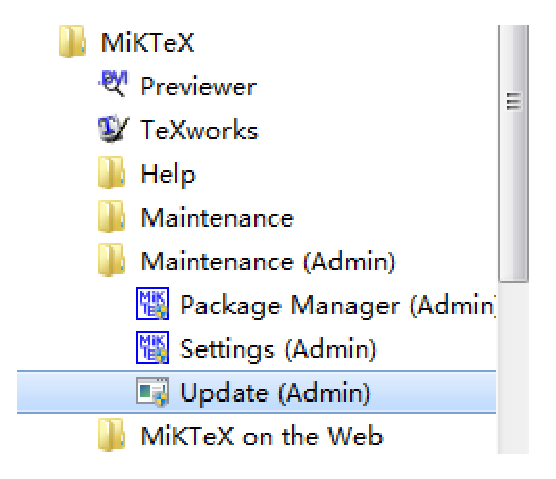
\includegraphics[scale=0.5]{./Pictures/set1.eps}\\
\caption{MiKTeX��������}
\label{set1}
\end{figure}

\begin{figure}[th]
\centering
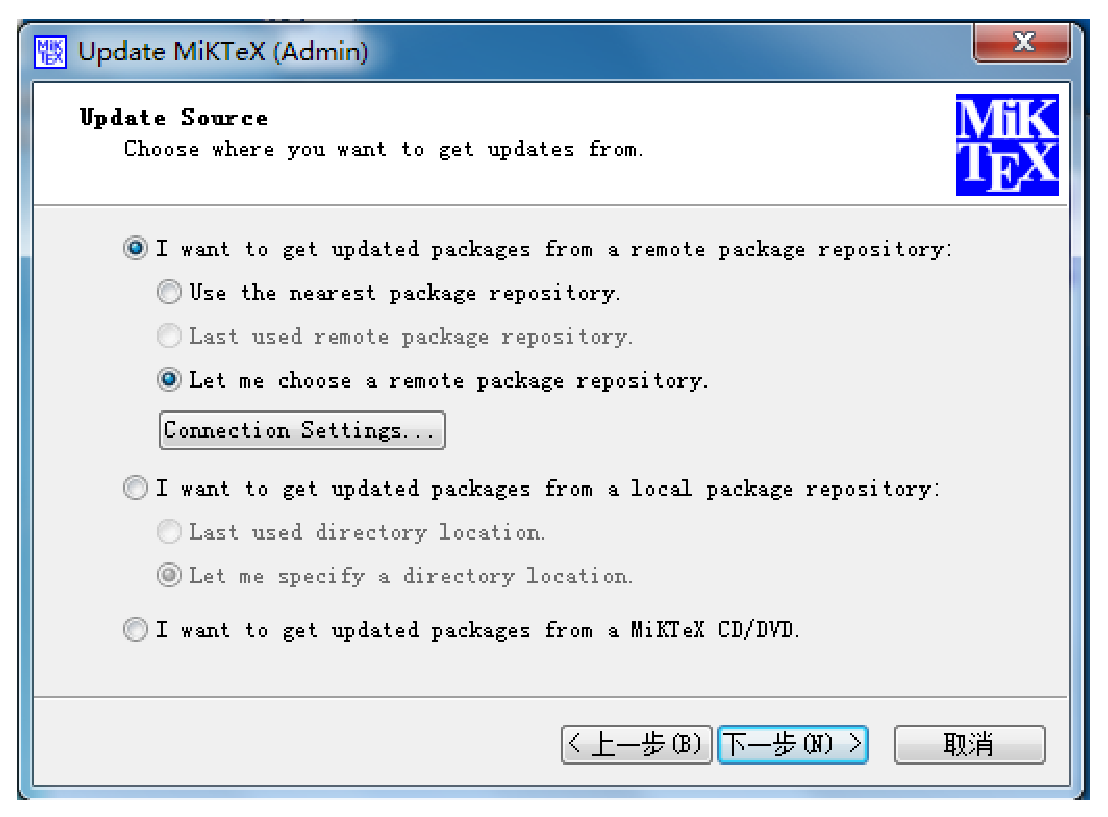
\includegraphics[scale=0.5]{./Pictures/set2.eps}\\
\caption{ѡ��������ʽ����ͼ��ѡ��һ������վ��}
\label{set2}
\end{figure}

\begin{figure}[th]
\centering
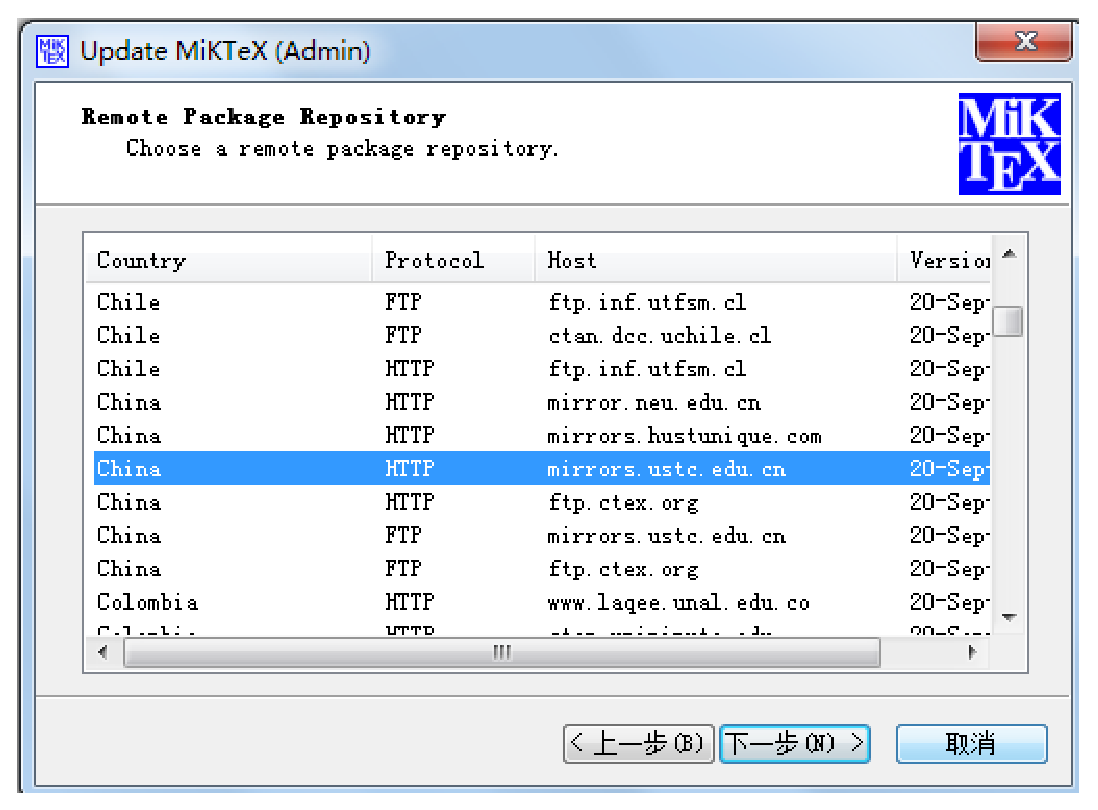
\includegraphics[scale=0.5]{./Pictures/set3.eps}\\
\caption{ѡ������վ�㣬���пƴ����Ϊ��}
\label{set3}
\end{figure}

֮����Ҫ��������������������Ϊ��ģ��ʹ�������µ�hyperref�������ӵ�����hidelinks��

\subsection{64λϵͳ}

����windows XP 64bit��Windows Server 2003 64bit��Vista 64bit��
Windows Server 2008 64bit��Windows 7 64bit �� Windows Server 2008 R2��

��װCTeX��װ��ʱ����Ҫѡ��MiKTeX�������������⣬��32λһ����
��װ��CTeX����ȥwww.miktex.org��վ����MiKTeX������64λ�棬��ǰ��2.9�棬
��װ��������ҳ���а�CTeX��Ŀ¼�ӵ�MiKTeX��RootĿ¼��ȥ����ͼ \ref{setroot} ��
����ͼ \ref{rffndb} ��ʾ��ˢ��MiKTeX��Ŀ¼���ݿ⣬�Ϳ���ʹ��CTeX�Ļ����ˡ�

\begin{figure}[thp]
\centering
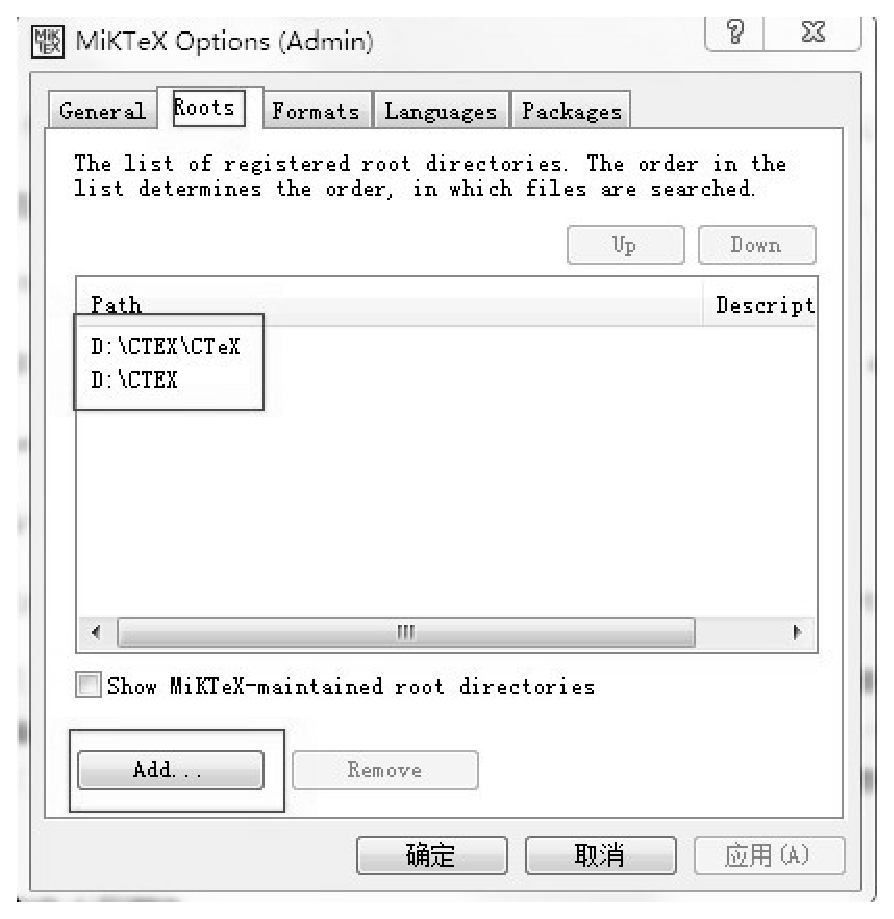
\includegraphics[scale=0.5]{./Pictures/setroot.eps}\\
\caption{����MiKTeX������RootĿ¼}
\label{setroot}
\end{figure}

\begin{figure}[th]
\centering
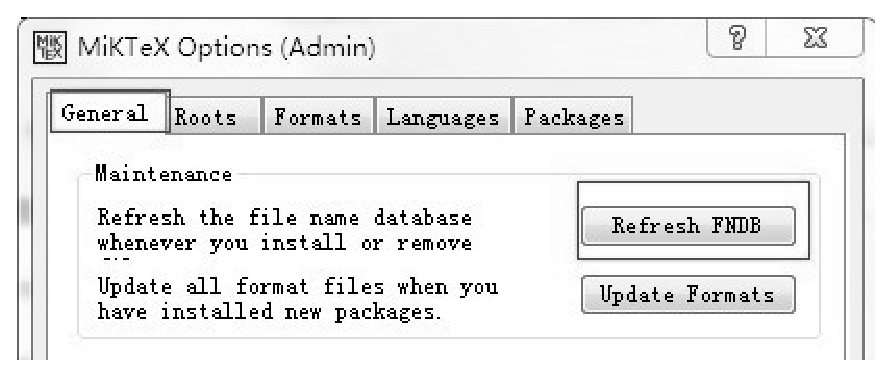
\includegraphics[scale=0.5]{./Pictures/rffndb.eps}\\
\caption{ˢ��MiKTeX��Ŀ¼���ݿ�}
\label{rffndb}
\end{figure}

��32λWindowsϵͳ��ͬ����װ���Ҳ��Ҫ��MiKTeX���������¡�

\section{linuxϵͳ}

������ѡ��\LaTeX ��װ�汾��Ȼ���CTeX�������뼴�ɡ�������linux��Ӧ�ö�������ɡ�
���ΰ汾ʹ�õIJ���ϵͳ������������Debian 6��TeXLive2009��

�뱣֤��չ���汾�㹻�¡�������hyperref������֤��2011��8�·ݺ�İ汾��

\section{Macϵͳ}

������ѡ��\LaTeX ��װ�汾������CTeX������ͬlinux�¡�

\section{��ģ������Ҫ����չ��}

\begin{enumerate}

\item{ͼ�Ρ���������չ��} graphicx��array��booktabs��caption��natbib��multirow

\item{��������չ��} times(\LaTeX{}��������)��fontspec(\XeTeX{}��������)

\item{Ŀ¼ѡ����չ��} tocbibind��tocloft��makeidx��hyperref

\item{��ѧ��ʽ��չ��} amsmath��amsthm��amsfonts��amssymb��bm

\end{enumerate}

\section{��������}

����Ѿ���װ����CTeX������\LaTeX ��������ô�������������ģ���ļ������makethesis.bat�ļ���
�����ӵ�ʮ��������������һ�ݽ���������ģ��ʾ��.pdf�����ĵ�����ô����ϲ�����ģ������Ҫ���������������ɹ���
���û��������һ���ļ�����ô�п��������������û��������ȷ�������\LaTeX �������������£�
���ģ������Ҫ����չ��û�б���װ�����\LaTeX �����Զ��������ܣ�
��֤\LaTeX �����ܹ��ɹ������ӵ�CTANվ�������������չ���ܰ���


\chapter{ʹ�ø�ģ��}

���濪ʼ�������ʹ�����ģ�棬�������Ѿ������
���ģ���Ŀ�ľ�����û��һ��\LaTeX ������ͬѧҲ�ܺܿ����\LaTeX ��֯���Լ������ġ�
��ˣ����ģ��û�й����ѡ�ֻ��һЩ��дWordͬ���Ѷ�\footnote{�ǵģ��Ѷ��ٺܶ�ܶࡣ����һ�������õĽ�ע}��ע�����
���ѵ㣬Ҫ��Word�ٺܶࡣ

���ģ��һ����Ҫ���¼����ļ���
\begin{enumerate}
\item{ZJUthesis.cls}�������ģ���ļ���
\item{ZJUthesis.cfg}�������ģ��������ļ�����ģ���ļ����ʹ�ã�
\item{ZJUthesis.bst}������Dzο����׵ĸ�ʽ˵���ļ���
\item{�ļ���CoverPagepic}������ŷ���ʹ�õ������У����У��ͼƬ��
\item{CoverPagepic$\backslash$ZJDX.eps}��eps\index{eps}��ʽ\footnote{����eps��ʽ��
ͼƬһ���н�������һ������}�����У��ͼƬ��
\item{CoverPagepic$\backslash$ZJDX.pdf}��pdf��ʽ\footnote{ͬeps����}�����У��ͼƬ��
\item{CoverPagepic$\backslash$QSY.eps}��eps��ʽ��У�գ�
\item{CoverPagepic$\backslash$QSY.pdf}��pdf��ʽ��У�ա�
\item{Chapter$\backslash$Copyright.tex}������ǰ�Ȩת��������
\item{Signature$\backslash$sign\_ch.eps���߸�ǩ���ļ�}�����������ǩ����Ĭ����һ���հ׵�eps���ύ���հ��ʱ��ɽ����滻Ϊ��Ӧ��ǩ��ͼƬ��ֱ�ӿ�������pdf�ĵ���ȥ�����߸��ļ�ͬ���������Ӧ��pdf��ʽͼ���ļ������ļ�������Ӧǩ����Ӧ���£�

{
\zihao{5}
\begin{tabular}{cl}
sign\_ch & ���ߵ�����ǩ������������ҳ�ã�\\
sign\_ch\_s & ��ʦ������ǩ������������ҳ�ã�\\
sign\_en & ���ߵ�Ӣ��ǩ����Ӣ������ҳ�ã�\\
sign\_en\_s & ��ʦ��Ӣ��ǩ����Ӣ������ҳ�ã�\\
sign\_cr\_1 & ���ߵ�����ǩ������Ȩ����ҳ�ã�\\
sign\_cr\_2 & ���ߵ�����ǩ������Ȩ����ҳ�ã�\\
sign\_cr\_s & ��ʦ������ǩ������Ȩ����ҳ�ã�\\
\end{tabular}
}

��Ȼ�����м���ǩ��������ͬһ���ļ�����ʹ�á�Ҳ�������߸���ͬ��ʹ�á�
Ҫע�����ǩ����ͼ���ļ������ȴ�Լ������2:1��
\end{enumerate}

���ڼ�������winEdt��������ϰ��ʹ�õ��ı��༭����
������ĵ���texԴ�ļ������ǽ���������ģ��ʾ��.tex��������ļ���
������д���ģ�����д����һ����չ��Ϊ��tex���Ĵ��ı��ļ���

�������ڿ�ʼ���ĵ�һ�С�

\section{ģ��ѡ��}

%$\backslash$documentclass[oneside]\index{oneside}\{ZJUthesis\}
{\noindent\zihao{-5}\verb+\documentclass[oneside]{ZJUthesis}+}

��һ���ָ��������ĵ����õĸ�ʽģ�棬������������ģ�棬{\bf ZJUthesis}
�������ģ���ļ����ļ�����
��{\bf$\backslash$documentclass}����һ�������\LaTeX Դ�ļ��У�
��б��$\backslash$��ͷ�ĵ���ĸ�ַ���������һ�����
����ֻ����һ��б�߼���������ַ������ɣ����ܰ����������������ţ�
����������ĸ�������ַ�ʱ�����������ַ�����������ˣ�{\bf$\backslash$documentclass}
��һ������������������ݡ�������IJ��������DZ�������
\{\}�еġ�ZJUthesis��������������˵�����ĵ�ʹ�õĸ�ʽģ�档��[oneside]����{\bf ZJUthesis}
���ģ��IJ��������������ʾ���������ڲ��õ���ӡˢģʽ��

���ģ��˵���ṩ�Ŀ���ѡ��ֻ��������һ�����ĵĵ�˫��ģʽ����һ���������������ӵ���ɫ��
�������ĵĵ���ģʽ��ͨ����
$\backslash$documentclass[oneside]\{ZJUthesis\}�в����[oneside]��ʵ�ֵģ�
����[oneside]����[twoside]\index{twoside}����ɾ��ʱ�����ľͱ����˫��ģʽ��

����԰�����˵�İ����˵���ĵ��ij�˫��ģʽ��Ȼ�󱣴棬������makethesis.bat�����ɳ����ġ�����ģ��ʾ��.pdf��\footnote{�����µġ�����ģ��ʾ��.pdfʱ��������ļ������򿪣����ȹرա�������ܲ��������µ��ļ�����}������������ģʽ�кβ�ͬ��

�����������ǵ��滹��˫�棿ѡ����������򵥣�

��texԴ�ļ��У���\%��ͷ���ж���ע���У�����������ʱ����Щ�н����ᱻ���İ�����
���ԣ���������ע������дһЩ������������һЩ���ֵ���ע������һ��������ʱ���Ž�ȥ��
����ɾ�����ǣ�ֻ��Ҫ������ע�͵�������������

{\zihao{-5}
\begin{verbatim}
% ��һ�λ�����ʱ�Ȳ��ŵ������
��һ�λ��������������
\end{verbatim}
}
���Ǽ������¿���

�������ǿ����˵ڶ������������ӵ���ɫ������

%$\backslash$hypersetup\{colorlinks=false\}
{\noindent\zihao{-5}\verb+\hypersetup{colorlinks=false}+}

����˵���������ģ��������ĵ��е����ӣ�����Ŀ¼���������ο����׵ı�ż�����ɫ��
�Ա�ʾ��������ž���������صĵط�ȥ����Ȼ��ӡ���ĵ�ʱ�����Dz���������������ɫ��
���ѡ��������Ŀ�ģ������ѡ�false���ij��ˡ�true������ô�����������һ��makethesis.bat��
��һ�����ɵġ�����ģ��ʾ��.pdf����Ŀ¼��֮ǰ�кβ�ͬ��

�������������ĵ��Ŀ�ʼ�������

%$\backslash$begin\{document\}
{\noindent\zihao{-5}\verb+\begin{document}+}

��ʾ��ʼ��


�ĵ��������

%$\backslash$end\{document\}
{\noindent\zihao{-5}\verb+\end{document}+}

��ʾ�����ĵ��������Ӧ

������

%$\backslash$fangsong
{\noindent\zihao{-5}\verb+\fangsong+}

��ʾ�����ĵ���������ʹ�÷������塣
С���ֺ��Ѿ���ģ�������ú��ˣ��˴��������á�

\section{���ķ���������Ϣ}

�����Ѿ���ģ������������ֻ��������Ӧ��Ϣ���ɡ�

\vspace{8pt}

{\linespread{1}
\zihao{-5}\noindent
%$\backslash$classification\{TP311\} 
\begin{tabular}{p{5cm}p{10cm}}
\verb+\classification{TP311}+
&
\parbox[t]{10cm}{��ͼ����ţ���רҵ����ž�������� \\
http://grs.zju.edu.cn/News/html/grs/xwsqjgf/xwsq/xwsq\_{}bszn/2008-09-24/282-20080924085824.html ��ѯ��}\\

%$\backslash$serialnumber\{10335\}
\verb+\serialnumber{10335}+
&
��λ���룬�����10335��\\

%$\backslash$SecretLevel\{����\} 
\verb+\SecretLevel{����}+
&
���ܼ������û�У��Ͳ�д��һ�䣬�����ϾͲ�����ֱ��ܼ���\\

%$\backslash$PersonalID\{1234567\}
\verb+\PersonalID{1234567}+
&
����ţ�һ���Ǹ���ѧ�š�\\

%$\backslash$title\{��Һã�����������\} 
\verb+\title{��Һã�����������}+
&
��������\\

%$\backslash$titletl\{����һ��д����\}
\verb+\titletl{����һ��д����}+
&
���������̫��һ��д���£��������д������д�ڶ�����Ŀ��
���һ�о�д���£���һ�䲻�ó��֡�\\
\end{tabular}
}

\vspace{8pt}

��������������У���������ע�����г��ȵķ��䡣

\begin{center}
  \begin{tabular}{rl}
    {\bf\fangsong\zihao{-4}����������Ŀ:} 
    &
    \bf\fangsong\zihao{5} \ZJUunderline[180pt]{���ǵ�һ���ұȵڶ��г�} \\[0mm]
    &
    \bf\fangsong\zihao{5} \ZJUunderline[180pt]{���ǵڶ����Ҷ�} \\[0mm] 
  \end{tabular}
\end{center}

\begin{center}
  \begin{tabular}{rl}
    {\bf\fangsong\zihao{-4}����������Ŀ:} 
    &
    \bf\fangsong\zihao{5} \ZJUunderline[180pt]{���ǵ�һ���Ҷ�} \\[0mm]
    &
    \bf\fangsong\zihao{5} \ZJUunderline[180pt]{���ǵڶ����ұȵ�һ�г�} \\[0mm] 
  \end{tabular}
\end{center}

��������Ŀ���ȷ��䣬���������ա�

\vspace{8pt}

{\linespread{1}
\zihao{-5}\noindent
\begin{tabular}{p{5cm}p{10cm}}
%$\backslash$englishtitle\{Thesis Title\}
\verb+\englishtitle{Thesis Title}+
&
����Ӣ����\\

%$\backslash$englishtitletl\{Second Line\}
\verb+\englishtitletl{Second Line}+
&
ͬ�������������̫��һ��д���£�����д�ڶ��С�
���һ��д���£���һ��Ҳ���ó��֡�\\

%$\backslash$Author\{�����ڴ�\} 
\verb+\Author{�����ڴ�}+
&
�������������Լ������֡�\\
\end{tabular}
}

\vspace{8pt}

����������ָ�����֮���и���࣬������ʾЧ����

\begin{center}
  \begin{tabular}{l@{��}r}
    \zihao{-4}���������� & \fangsong\zihao{4}\ZJUunderline[160pt]{��\hspace{1.5em}��\hspace{1.5em}��}\\
  \end{tabular}
\end{center}

������д������ʱ�����¸�ʽ��д��

%$\backslash$Author\{��$\backslash$hspace\{1.5em\}��$\backslash$hspace\{1.5em\}��\}
{\noindent\zihao{-5}
\verb+\Author{��\hspace{1.5em}��\hspace{1.5em}��}+}

���е� $\backslash$hsapce\{{\bf1.5em}\} ��ʾ�ռ���Ϊ{\bfseries һ�����ַ�}��
���Ҫ{\bfseries һ���ַ�}��࣬��д{\bf 1em}\footnote{$\backslash$hsapce\{1em\}Ҳ����д��$\backslash$quad��}��{\bfseries �����ַ�}�ļ�࣬����{\bf 2em}���Դ����ơ�

\vspace{8pt}

{\linespread{1}
\zihao{-5}\noindent
\begin{tabular}{p{8cm}p{7cm}}
%$\backslash$degree\{ijʿ\} 
\verb+\degree{ijʿ}+
&
ʲôѧλ�����ģ��˶ʿ�����ߡ���ʿ����\\

%$\backslash$supervisor\{��ʦ����$\backslash$hspace\{1em\}ְ��\}
\verb+\supervisor{��ʦ����\space{1em}ְ��}+
&
�ʦ������ְ�ƣ�
����Լ���������ƣ���������м�Ҫ����հף���ο��Լ������пհ׵IJ��뷨��\\

%$\backslash$cpsupervisor\{������ʦ����$\backslash$hspace\{1em\}ְ��\} 
\verb+\cpsupervisor{������ʦ����\hspace{1em}ְ��}+
&
����к�����ʦ��
ʹ��������û�У��Ͳ�д���������������ݻ��Զ����е����������ֺ�����ʦ������\\

%$\backslash$major\{��������\}
\verb+\major{��������}+
&
�����Լ���רҵ���ƣ����ּ����ӿո�
����������ո����ӷ�����\\

%$\backslash$researchdm\{�����\} 
\verb+\researchdm{�����}+
&
�����Լ����о�����\\

%$\backslash$institute\{��������ѧԺ\}
\verb+\institute{��������ѧԺ}+
&
�����Լ���ѧԺ���ơ�\\

%$\backslash$submitdate\{2011��10��10��\}
\verb+\submitdate{2011��10��10��}+
&
���������ύ���ڣ���������д��\\

%$\backslash$defenddate\{2011��11��1��\} 
\verb+\defenddate{2011��11��1��}+
&
���Ǵ�����ڣ���������д�����ݸ�ʱ����
���Զ����ա�\\
\end{tabular}
}

\vspace{8pt}

���������������д��ϣ�����ʹ�����ɷ��������
%\begin{center}
%$\backslash$makeCoverPage
%\end{center}

{\noindent\zihao{-5}\verb+\CoverPagepic+}


�����ɷ��档

\section{ʵս�������Լ������ĵ�һҳ}

��������Ľ��ܣ���ô���Dz����Ѿ�ԾԾ����׼�����Լ������Ĵӵ�һҳ��ʼ�ˣ�����Ϳ�ʼ���ְɡ�

���ȣ���׼��һ���ļ��з���������ص������ļ������������ɡ��ҵı�ҵ���ġ���
Ȼ�󣬰ѡ�ʹ�ø�ģ�桱һ�����ᵽ�ļ���������ļ����������ҵı�ҵ���ġ��ļ�����ȥ��
���ţ�ʹ��WinEdt���������ı��༭�����ڡ��ҵı�ҵ���ġ��ļ����н���һ����չ��Ϊtex���ļ���
�ļ����Լ�ȡ���������ԡ�LATEX����ģ��ʹ��˵����Ϊ�ļ�����
��󣬱༭��LATEX����ģ��ʹ��˵��.tex��Ϊ�������ݣ�����Ԫ��������������д��

\vspace{5mm}

{
\linespread{1}
\noindent\zihao{-5}
%$\backslash$documentclass\{ZJUthesis\}
%$\backslash$hypersetup\{colorlinks=false\}
%$\backslash$begin\{document\}
%$\backslash$classification\{TM863\}
%$\backslash$serialnumber\{10335\}
%$\backslash$SecretLevel\{����\}
%$\backslash$PersonalID\{1234567\}
%$\backslash$titel\{������Ŀ\}
%$\backslash$titletl\{������Ŀ�ڶ���\}
%$\backslash$englishtitle\{English Title\}
%$\backslash$englishtitletl\{Second Line\}
%$\backslash$Author\{����\}
%$\backslash$supervisor\{��ʦ����\}
%$\backslash$cpsupervisor\{������ʦ����\}
%$\backslash$major\{רҵ����\}
%$\backslash$researchdm\{�����\}
%$\backslash$institute\{����ѧԺ\}
%$\backslash$submitdate\{�ύ����\}
%$\backslash$defenddate\{�������\}
%$\backslash$makeCoverPage
%$\backslash$end\{document\}
\begin{verbatim}
\documentclass{ZJUthesis}
\hypersetup{colorlinks=false}
\begin{document}
\classification{TM863}
\serialnumber{10335}
\SecretLevel{����}
\PersonalID{1234567}
\titletitel{������Ŀ}
\titletl{������Ŀ�ڶ���}
\englishtitle{English Title}
\englishtitletl{Second Line}
\Author{����}
\supervisor{��ʦ����}
\cpsupervisor{������ʦ����}
\major{רҵ����}
\researchdm{�����}
\institute{����ѧԺ}
\submitdate{�ύ����}
\defenddate{�������}
\makeCoverPage
\end{document}
\end{verbatim}
}

�������ݿ���ֱ�Ӵӡ�����ģ��ʾ��.tex���п����������鱣�����е�ע�Ͳ��֡�
��дtexԴ�ļ��У����龡���ܶ���ע�ͣ��Է�������޸ġ�

��һ��ע��ĵط��ǣ����һ��һ��Ҫ�� {\bf$\backslash$end\{document\}}��
����԰ѡ�����ģ��ʾ��.tex�����������棬������������Dz��Ǿ�������һ�䡣

\begin{figure}{thb}
\centering
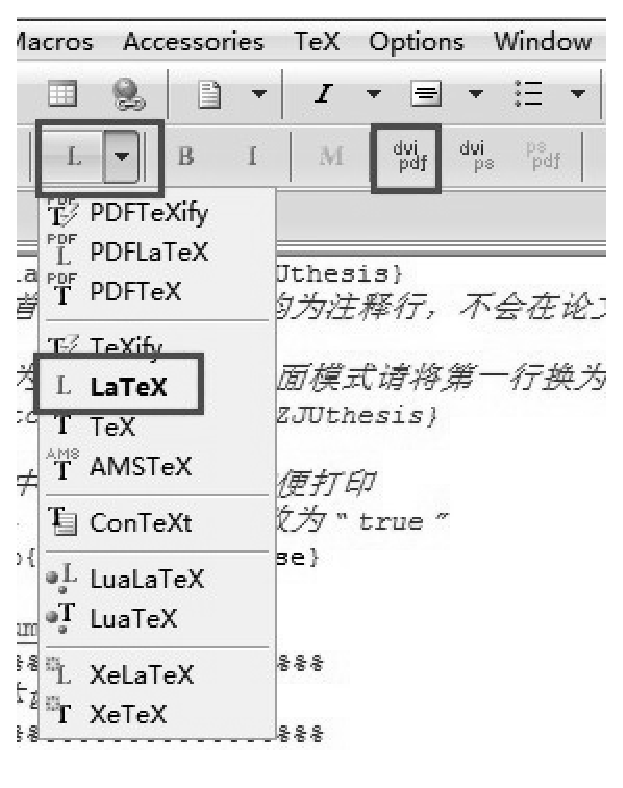
\includegraphics[scale=0.8]{./Pictures/runLaTeX.eps}
\caption{����LaTeX}
\label{runLaTeX}
\end{figure}

Ȼ����WinEdt�������е�LaTeX�����Լ����������ɺ�
�ٵ��ұߵ�dvipdf��ť����ͼ \ref{runLaTeX} ��ʾ���Ϳ�������
��LATEX����ģ��ʹ��˵��.pdf�����򿪾Ϳ��Կ������ɵķ����ˡ�

�㡰LaTeX����ť��ʱ��Ҫע����ǣ����ұߵ�С��ͷȻ���������IJ˵���ֻ����ѡ��ij������˴�ѡ��LaTeX����
Ҫִ��Ҫ�㵽��ť�ϲ��С�

�����Դ���һ���������ļ������������񣬴˴��������ļ��������£�

%\vspace{4mm}
{\linespread{1}
\zihao{-5}
\begin{verbatim}
latex --src-specials --synctex=-1 LATEX����ģ��ʹ��˵��
dvipdfmx -p a4 LATEX����ģ��ʹ��˵��
\end{verbatim}
}
\vspace{4mm}

��ǰĿ¼�������������������Ҳ�����е���LATEX����ģ��ʹ��˵��.pdf���ļ���

����Ҫ˵����һ���ǣ���������п�ʼ����ο����ף���������Ϣ��
��ô����pdf�ĵ������̻�Ҫ���ӣ�ʹ��WinEdt����˳���ǣ��ȵ����LaTeX�����ť��
�ٵ���ұߵġ�B����ť�����ɲο�������Ϣ�ļ����͡�I����ť������������Ϣ�ļ�����
Ȼ��{\bfseries ��}�����LaTeX������{\bfseries ����}������ٽ���dvi��pdf��ת����
�������ɵ�pdf�ļ��вο����������������ô����ǡ������š�
��ʹ���������������ɣ�����Ӧ���������ļ�����Ӧ�޸����£�

%\vspace{4mm}
{\linespread{1}
\zihao{-5}
\begin{verbatim}
latex --src-specials --synctex=-1 LATEX����ģ��ʹ��˵��
makeindex LATEX����ģ��ʹ��˵��.idx
bibtex LATEX����ģ��ʹ��˵��
latex --src-specials --synctex=-1 LATEX����ģ��ʹ��˵��
latex --src-specials --synctex=-1 LATEX����ģ��ʹ��˵��
dvipdfmx -p a4 LATEX����ģ��ʹ��˵��
\end{verbatim}
}
\vspace{4mm}

\section{�������ҳ��Ϣ}

���Ͻ��Ѿ�����˷������Ϣ�����봴�����������ǽ�������ҳ�Ĵ�����
�봴������ҳһ��������ҳҲ����������Ϣ���ٴ���ҳ�档

���ǻص�������ģ��ʾ��.tex���У�
����ҳ����������ҳ��Ӣ������ҳ��
������������ҳҪ�������Ϣ����������������ίԱ��������
��Ȼ�������ڲݸ�׶��⼸����Ϣ�Dz���ģ����������ɣ�
�����������ĵ��Ӹ�ʱ������д��Щ��Ϣ��

������������Ϣ���뼰˵�����£�

\vspace{8pt}
{
\linespread{1}
\zihao{-5}\noindent
\begin{tabular}{ll}
\verb+\reviewersA{��\hspace{1em}��\hspace{1.5em}ְ��\hspace{1.5em}��λ}+ & ����������1\\
\verb+\reviewersB{������\hspace{1.5em}ְ��\hspace{1.5em}��λ}+ & ����������2\\
\verb+\reviewersC{������\hspace{1em}����ְ\hspace{1em}��λ}+ & ����������3\\
\verb+\reviewersD{��\hspace{1em}��\hspace{1.5em}ְ��\hspace{1.5em}��λ}+ & ����������4\\
\verb+\reviewersE{��\hspace{1em}��\hspace{1.5em}ְ��\hspace{1.5em}��λ}+ & ����������5\\
\end{tabular}
}
\vspace{8pt}

Ϊ��ʹ�ⲿ����Ϣ�Ű����ۣ�����Ҫע��һ�㣺

�滮�á�����������ְ�ơ�������λ����ռ�Ŀռ䣬��λ����ռ�ÿռ�
������Ҫ����ʮ�����֡�
���磺

\begin{center}
\begin{tabular}{l@{��}r}
����������1
&
\ZJUunderline[220pt]{��\hspace{1em}��\hspace{1.5em}ְ��\hspace{1.5em}�����λ���Ƚϳ�����}\\
����������2
&
\ZJUunderline[220pt]{������\hspace{1.5em}ְ��\hspace{1.5em}�����λ����\hspace{4em}}\\
����������3
&
\ZJUunderline[220pt]{������\hspace{1em}��ְ��\hspace{1em}�����λ�����ܳ�\hspace{2em}}\\
\end{tabular}
\end{center}

��Ҫ��

\begin{center}

\begin{tabular}{l@{��}r}
����������1
&
\ZJUunderline[220pt]{����\hspace{1em}ְ��\hspace{1em}�����λ���Ƚϳ�����}\\
����������2
&
\ZJUunderline[220pt]{������\hspace{1em}ְ��\hspace{1em}�����λ����}\\
����������3
&
\ZJUunderline[220pt]{������\hspace{1em}��ְ��\hspace{1em}�����λ�����ܳ�}\\
\end{tabular}
\end{center}

������Ҫ�õöࡣ

ǰ�ߵĴ������£�
{\linespread{1}
\zihao{-5}
\begin{verbatim}
\reviewersA{��\hspace{1em}��\hspace{1.5em}ְ��\hspace{1.5em}�����λ���Ƚϳ�����}
\reviewersB{������\hspace{1.5em}ְ��\hspace{1.5em}�����λ����\hspace{4em}}
\reviewersC{������\hspace{1em}��ְ��\hspace{1em}�����λ�����ͺܳ�\hspace{2em}}
\end{verbatim}
}

ע��$\backslash$space{Xem}���÷���һ��em����һ���ֿ��������е�λ����䵽ͬһ���ȣ�
��ĵ�λ����10���֣�6���ֵĵ�λ����Ҫ��4��em��8���ֵĵ�λ����2��em��
����ݾ���������е�����

���ίԱ����Ϣ���뼰˵�����£�

\vspace{8pt}
{
\linespread{1}
\zihao{-5}\noindent
\begin{tabular}{ll}
\verb+\chairman{��\hspace{1em}��\hspace{1.5em}ְ��\hspace{1.5em}��λ}+ & ���ίԱ����ϯ\\
\verb+\commissionerA{������\hspace{1.5em}ְ��\hspace{1.5em}��λ}+ & ���ίԱ���Ա1\\
\verb+\commissionerB{������\hspace{1em}����ְ\hspace{1em}��λ}+ & ���ίԱ���Ա2\\
\verb+\commissionerC{��\hspace{1em}��\hspace{1.5em}ְ��\hspace{1.5em}��λ}+ & ���ίԱ���Ա3\\
\verb+\commissionerD{��\hspace{1em}��\hspace{1.5em}ְ��\hspace{1.5em}��λ}+ & ���ίԱ���Ա4\\
\verb+\commissionerE{��\hspace{1em}��\hspace{1.5em}ְ��\hspace{1.5em}��λ}+ & ���ίԱ���Ա5\\
\end{tabular}
}

\vspace{8pt}

���ίԱ����Ϣͬ���滮��������ְ�ƣ���λ��Ϣ���滮��������������ͬ��

������������ҳ

\vspace{8pt}
\verb+\maketitle+
\vspace{8pt}

�����ļ�������PDFԤ��Ч����

Ӣ������ҳ��Ϣ��������������ҳ���ơ�

�˴�Ӣ��������������һ�Σ�ͬ�����һ��д����д�����С����з��������д�����

{
\linespread{1}
\zihao{-5}\noindent
\begin{tabular}{p{7cm}l}
\verb+\Etitle{English Title}+ & Ӣ�ı���\\
\verb+\Etitletl{Second Line}+ & ���һ��д���£�����д�ڶ���\\
\end{tabular}
}

Ӣ������ҳ������������ίԱ����Ϣ��˵�����£�

{
\linespread{1}
\zihao{-5}\noindent
\begin{tabular}{ll}
\verb+\EreviewersA{Name\hspace{1.5em}Professional Title\hspace{1.5em}Organization}+ & ����������1\\
\verb+\EreviewersB{Name\hspace{1.5em}Professional Title\hspace{1.5em}Organization}+ & ����������2\\
\verb+\EreviewersC{Name\hspace{1.5em}Professional Title\hspace{1.5em}Organization}+ & ����������3\\
\verb+\EreviewersD{Name\hspace{1.5em}Professional Title\hspace{1.5em}Organization}+ & ����������4\\
\verb+\EreviewersE{Name\hspace{1.5em}Professional Title\hspace{1.5em}Organization}+ & ����������5\\
\verb+\Echairman{Name\hspace{1.5em}Professional Title\hspace{1.5em}Organization}+ & ���ίԱ����ϯ\\
\verb+\EcommissionerA{Name\hspace{1.5em}Professional Title\hspace{1.5em}Organization}+ & ���ίԱ���Ա1\\
\verb+\EcommissionerB{Name\hspace{1.5em}Professional Title\hspace{1.5em}Organization}+ & ���ίԱ���Ա2\\
\verb+\EcommissionerC{Name\hspace{1.5em}Professional Title\hspace{1.5em}Organization}+ & ���ίԱ���Ա3\\
\verb+\EcommissionerD{Name\hspace{1.5em}Professional Title\hspace{1.5em}Organization}+ & ���ίԱ���Ա4\\
\verb+\EcommissionerE{Name\hspace{1.5em}Professional Title\hspace{1.5em}Organization}+ & ���ίԱ���Ա5\\
\end{tabular}
}

ͬ��������ҳ���ƣ������������ְ�ƣ���λ��Ϣ�����ü�д������Ӣ��һ�п��ܻ�д���¡�
���⣬����֮��ļ��������������գ���������Ϣ�����Ʒ�ʽһ�¡�

���ˣ�Ӣ������ҳ��Ϣ������ϡ���Ӣ������ҳ��������Ӣ������ҳ

\vspace{8pt}
\verb+\makeEtitle+
\vspace{8pt}

����{\bfseries ��Ҫ����}����{\bfseries ��Ȩ��Ϣҳ}

{
\zihao{5}
\begin{verbatim}
\SignautreDateA{2013}{10}{11}
\SignautreDateB{2013}{10}{11}
\SignautreDateC{2013}{10}{11}
\makeOSandCPRTpage
\end{verbatim}
}

���������ʱ�������Ӧ��Ȩ��Ϣҳ�е�ǩ��������Ϣ��
�ڲݸ弰����׶Σ��⼸��������Բ�д�����Զ����⼸��λ�����ա�

\section{���IJ��ָ��½ڵ���д}

�Դˣ����ĵķ��棬����ҳ��汾��Ϣҳ������ϣ���ʼ�����������ĵ���д�׶Ρ�
��������ݽ�����������Ϊ�����������Լ�����������Ϊ����

���ǻص�������ģ��ʾ�����������IJ��ֵĿ�ʼ�����ǿ�������һ�����

\verb+\ZJUfrontmatter+

����������˼�ǿ�ʼ���ĵ����IJ��֣���ҳ������Ϊ��д�������֣�����I��ʼ��


��̸������ʹ��֮ǰ��д��̸һ�����ݲ��ֵ���д��
\LaTeX ������������дû��ʲô�ر�ĸ�ʽ��ֱ����д���ɡ�
����Ҫע�����¼��㣺

\begin{enumerate}
\item{\LaTeX ����������ַ���Ŀո�Ҳ����˵��}

{
\linespread{1}
\zihao{-5}
\vspace{8pt}
\noindent\verb+��Һã��ҵ��м�û�пո�+\\
{\zihao{-4}��}\\
\verb+�� �� �ã� ��  ��    ��   �� û �� ��      ��+
\vspace{8pt}
}

��������������һ���ġ����ǣ�

��Һã��ҵ��м�û�пո�

����������ַ����������ĵı����ţ������������������ȡ�

�����Ҫ�����ĵ��ʼ����ո���ô�죿ֻ��Ҫ�á�\~{}��������ո񣬾���������

{
\linespread{1}
\zihao{-5}
\vspace{8pt}
\noindent\verb+��~��~�ã�~��~��~��~���кܶ�Ŀ�~��+
\vspace{8pt}
}

����������������ˣ�

��~��~�ã�~��~��~��~���кܶ�Ŀ�~��

����Ӣ�ĵ���ǰ��Ŀո�\LaTeX ��{\bfseries ����һ��}��

\item{������ֶ�}

\LaTeX �У�{\bfseries ����һ���س�}Ҳ����ո�һ�������ԣ�������Ϊ�ֶεı�־��
����������е�Ч��һ�����С����⣬����һ���������
��$\backslash$$\backslash$���������ǡ�$\backslash$linebreak����
��������������ֱ�ӻ��е����ֶΣ����»�����ǰ�������񡣱���

{
\linespread{1}
\zihao{-5}
\vspace{8pt}
���ǵ�һ�У�\\
�һ��ǵ�һ�С�

���ǵ�һ�Σ�

���ǵڶ��Ρ�

\begin{verbatim}
���ǵ�һ�У�\\
���ǵڶ��С�
\end{verbatim}
\vspace{8pt}
}

���������������

\vspace{8pt}

\hspace{2em}���ǵ�һ�У�
�һ��ǵ�һ�С�

\hspace{2em}���ǵ�һ�Σ�

\hspace{2em}���ǵڶ��Ρ�

\hspace{2em}���ǵ�һ�У�\\
���ǵڶ��С�

\vspace{8pt}

��ˣ��ڱ�д����tex�ļ���ʱ��ͬһ�����ڿ������⻻�У�
����дһ�仰�ͻ�һ�У������������Լ�д��ʱ��˼·��������
ֻҪ�������У�������ɵ��ļ�����һ���Ρ�

\item{��Ӣ�Ļ�ϱ༭ʱ��һ�����⼰�������}

���ijһ����������Ӣ���ַ���ϣ����纬�е��ʣ�
��ô�������һ�����⴦����\LaTeX ������PDFʱ���ܻ����ijһ�����һ��Ӣ�ĵ���ͻ�����⡣
����������İ취������Ӣ���ַ������ʵ�ǰ�漰������Ͽո���š�
��Ȼ��������̫���������Լ���д��ϰ�ߣ�һ����������Ҳ̫���¡�
û��ϵ��\LaTeX �������������Ѿ������Ǽ���������⡣
CCT�׼�����һ������cctspace.exe��ֻҪ�������¸�ʽ������:

\verb+cctspace [�����ļ���] [����ļ���]+

�Ϳ���ִ������ո����������������ֹ�һ��һ�����ӡ�

��������ڰ�װCTeX����ʱ�Ѿ�����װ����ֱ��ʹ�á�ʹ��linux��ͬѧ�ǣ��������ڲο������е���վ������Դ������롣

��������������Ĺ���ѡ��˵������ο����ֲ��ġ������°�CCT��˵����\cite{NewCCT:2006}��4.2�ڲ������ݣ�
�̵ܶģ�ֻ��һҳ��������˵���ĵ���


\item{������һЩҪע�������}

\LaTeX ���в���������Ų���ֱ�����룬���£�

\verb+#   $   %   ^   &   _   {   }   \+

��������Ҫ�����µ�����

\verb+\#   \$   \%   \^   \&    \_{}    \{    \}    $\backslash$+

\end{enumerate}

���Ͼ�����д������������ʱ��һЩ˵�������ೣ�����⣬��ο���һ�ݲ�̫��̵�\LaTeXe ���ܡ�\cite{LaTeXshzh}�͡�CTeX FAQ����
�������ĵ��������ڿ�ʼ--�˵�--����--CTeX--help���ҵ���


���½����½ڽ��ܸ�������дʱ���ʹ�ø�ģ�档

\subsection{����ҳ}

��ʵ����������������һ�����֣�����Ϊһ�����֣����ǽ���������ģ���ڡ��������Ҫ��ֱ�ӽ���ע�͵�����ɾ�����ɡ�

����ҳ�ĵ�������Ϊ

{
\linespread{1}
\zihao{-5}\noindent
\begin{verbatim}
\begin{corrigenda}
�����д��Ŀ������ݡ�
\end{corrigenda}
\end{verbatim}
}

��ͬѧ���ܻᷢ�֣��ڡ�����ģ��ʾ��.tex�����ⲿ�ֲ�����ôд�ģ����ڽ���������л�����н�����ԭ��

\subsection{��л}

��л�ĵ��������뿱��ҳ���ƣ�Ϊ

{
\linespread{1}
\zihao{-5}\noindent
\begin{verbatim}
\begin{thanks}
�����д�����л���ݡ�
\end{thanks}
\end{verbatim}
}

���ǿ�������ģ��ʾ��.tex������һ����ȴֻ�Ǽ�д��һ�䣺

\verb+\begin{thanks}
在我写这个文档的过程中,得到了网络上很多网贴的帮助,在此感谢baidu,Google,感谢
~CTeX 社区http://www.ctex.org,\LaTeX{}学习园地:http://blog.sina.com.cn/wangzhaoli11,
中科大~CTAN~镜像http://mirrors.ustc.edu.cn/CTAN/,水木社区\TeX{}版等网站、论坛,
其他一些较小的个人网站,论坛不再一一点名,在此一并感谢。
感谢浙江大学数学系提供的原始模版,感谢88\TeX{}版。
\end{thanks}
+

�����$\backslash$input����ָ������һ��tex�ļ������ݵ���ǰλ�ã�
����˵\LaTeX �ڱ������texԴ�ļ�ʱ���������ȥ������ָ������һ��tex�ļ���
������������ȫ�����Ƶ����λ�á�

�������ĺô���ʵ�������ĵ�ģ�黯�����԰����ĵIJ����½�д����ͬ���ļ���ȥ��
ÿ���ļ�������̫���������ײ鿴���޸ġ����������������ָ����ļ����ǵ�ǰĿ¼��ChaptersĿ¼�µ�
thanks.tex�ļ���ͬѧ�ǿ���ȥ��һ�£����thanks.tex�ļ��е����ݣ��Dz��Ǿ���
��������д��������һ���ġ�

Ҫע����ǣ��������Ŀ¼�����ļ�������Ϊ���ģ���������\footnote{linux�µ�ͬѧ����������}��

\subsection{����}

ʹ�÷���ͬ��л���������£�

{
\linespread{1}
\zihao{-5}\noindent
\begin{verbatim}
\begin{preface}
�����д������Ե����ݡ�
\end{preface}
\end{verbatim}
}

\subsection{ժҪ}

ժҪ����д����л���ƣ�ֻ����һ���ؼ�������$\backslash$keywords���������£�

{
\linespread{1}
\zihao{-5}\noindent
\begin{verbatim}
\begin{abstractC}
�����д���ժҪ�����ݡ�

\keywords{�ؽ���1���ؼ���2}
\end{abstractC}
\end{verbatim}
}

\subsection{Ӣ��ժҪ}

Ӣ��ժҪ���������ժҪ��ȫһ����ֻ�Ƕ�����Ӣ�ģ��������£�

{
\linespread{1}
\zihao{-5}\noindent
\begin{verbatim}
\begin{abstractE}
�����д���ժҪ�����ݡ�

\keywordsE{keywords1��keywords2}
\end{abstractC}
\end{verbatim}
}

����ط�Ҫע�����������ժҪ���֮ͬ����abstractE��keywordsE��

\subsection{ͼƬĿ¼}

��һ����ֻ��Ҫ����һ����������Ķ���\LaTeX �Լ�������㶨��

\verb+\ZJUListofFigures+

����㲻��ҪͼƬĿ¼����ô����������ɾȥ����ע�͵���

\subsection{����Ŀ¼}

��һ����ͬ��ֻ��Ҫ����һ����������Ķ���\LaTeX ���������á�

\verb+\ZJUListofTables+

����㲻��Ҫ����Ŀ¼��ͬ��ֻҪ����������ɾȥ����ע�͵����ɡ�

\subsection{��д�������嵥�������}

��һ��������л�������ơ��������£�

{
\linespread{1}
\zihao{-5}\noindent
\begin{verbatim}
\begin{ListofSymbol}
�����д�����д�������嵥������������ݡ�
\end{ListofSymbol}
\end{verbatim}
}

\subsection{Ŀ¼}

��һ����ֻ��Ҫ����һ�����\LaTeX ������㶨һ�С�

\verb+\ZJUcontents+

\subsection{�����½�����}

������͵��������½ڵı�д�ˡ����IJ���д������л�����Ե���ͬ��
����л������û�и�С�ķֽڣ�Ҳ������ͼƬ����������ݡ�
ͼƬ�������������ڱ�˵���з������漸���У�������ֻ�������ĵ��½��Ų���

�ڿ�ʼ��������֮ǰ����Ҫһ��\LaTeX ���������������������IJ��֣�
ҳ����Ҫ���´�1��ţ���ʹ�ð��������֣��Լ��½ڿ�ʼ��1��ʼ�����������

\verb+\ZJUmainmatter+

���Ļ��кܶ��£����������������������ۣ�����ʲô�ġ���дtex�ļ���ʱ��
��Ҫ��\LaTeX ��ȷ��Щ���£���Щ�ǽڣ���һЩ�Ǹ�С�Ľڡ�������\LaTeX ������ȷ�ظ�����������ݷ��£��ֽ�

�½ڱ������ʹ�����£�

{
\linespread{1}
\zihao{-5}\noindent
\begin{verbatim}
\chapter{�����µı���}
�����±����µ�����
\section{���ǵ�һ�ڵı���}
���ǽڱ����µ�����
\subsection{����С�ڵı���}
����С�ڵ����ݡ�
\begin{enumerate}
\item{���Dz�����1}
\item{���Dz�����2}
\end{enumerate}
\subsection{���ǵڶ�С�ڵı���}
���ǵڶ�С�ڵ����ݡ�
\section{���ǵڶ��ڵı���}
���ǵڶ��ڵ�����
\subsection{���ǵڶ��ڵ�һС�ڵı���}
���ǵڶ��ڵ�һС�ڵ�����
��������
\end{verbatim}
}

�½ڱ����в���Ҫ˵���ǵڼ��µڼ��ڣ�\LaTeX ��������㣬
����Ҫ����ֻ�ǰ�������°��ṹͳһ�������ɡ�
���ң�Ŀ��Ҳ�������ı��������Զ����ɡ�
����Ҫ����һ����ǣ��еı�����ܻ�Ƚϳ���д��Ŀ¼��ᵼ��Ŀ¼��Ŀ���У�
Ϊ���������⣬\LaTeX ����Ŀ¼�еı�����ʵ�ʵı��ⲻһ����Ҫ�ﵽ���Ч����
���µı���Ϊ����������Ӧ��һ�����������£�

\verb+\section[Ŀ¼�еı���]{ʵ���½��еı���}+

��ģ�����½ڼ��϶��������6�㣬�㹻���ˡ���� \ref{ChapsecList} ��ʾ��

\begin{table}[thb]
\zihao{5}
\caption{�½�����}
\label{ChapsecList}
\centering
\begin{minipage}[c]{9cm}
\centering
\begin{tabular}{p{6cm}|c}
\hline
���� & ���\\
\hline
\verb+\chapter+ & ��\footnote{ʵ�������µ��ϲ㻹��һ�����part�����֣�����ģ�����ò�����}\\
\hline
\verb+\section+ & ��\\
\hline
\verb+\subsection+ & ��\\
\hline
\verb+\subsubsection+ & СС��\\
\hline
\verb+\paragraph+ & ��\\
\hline
\verb+\subparagraph+ & �ֶ�\\
\hline
\end{tabular}
\end{minipage}
\end{table}

���⣬���ij����Ҫ�õ�������������Բ���enumberate�������������£�
{
\linespread{1}
\zihao{-5}\noindent
\begin{verbatim}
  \begin{enumerate}

  \item{���Dz�����1} 

  ���Dz�����1�����ݡ�

  ���潫��һ��Ƕ��Ӧ��

  \begin{enumerate}
    \item{���Dz�����1�е���һ��������1}

    ����С������1�����ݡ�

    \item{���Dz�����2�е���һ��������2}

    ����С������2�����ݡ�
  \end{enumerate}

  \item{���Dz�����2}

  ���Dz�����2�����ݡ�

  \end{enumerate}
\end{verbatim}
}

�����ĵ���Ч�����£�

\begin{enumerate}
\item{���Dz�����1}

���Dz�����1�����ݡ�

���潫��һ��Ƕ��Ӧ��

\begin{enumerate}
\item{���Dz�����1�е���һ��������1}

����С������1�����ݡ�

\item{���Dz�����2�е���һ��������2}

����С������2�����ݡ�

\end{enumerate}
\item{���Dz�����2}

���Dz�����2�����ݡ�

\end{enumerate}

\vspace{8pt}

ע��tex���벿���еĿ��С�

���ֲ�����ͬ������Ҫ���DZ�����⣬\LaTeX ����������һ�С�
Ƕ��Ӧ��������Ƕ�����㡣

\subsection{�����}

�����Դ�����ˣ�����������Ǻ���IJο����ף������������Ȳ��֡�
����Ҫһ����������������IJ��ֽ�������ʼ�ĺ󲿷�

\verb+\ZJUbackmatter+

�����IJ�����ɺ���һ�����־��Dzο����ס�
�ο����׵�������Ҫ׼������һ���ο����������ļ�*.bib��
��˵��������һ�������ļ����ӣ�thesis.bib��
���ļ�Ҳ��һ�����ı��ļ��������ü��±��򿪡�
������������ֲο����׵ĸ�ʽ��
ר����patent������׼��standard���������ĵ���Edoc����
�ڿ����ģ�article�����鼮��book������/˶ʿѧλ���ģ�mastersthesis/phdthesis����
�������ף�misc����

�������ڿ�����Ϊ����˵�����ĸ�ʽ��

{
\linespread{1}
\zihao{-5}\noindent
\begin{verbatim}
@article{
LUOZ:2007,
   Author = {���� and ��� and ��Сƽ and �����},
   Title = {����{LATEX}��ѧλ����ģ��������ʵ��},
   Journal = {�������չ�ҵѧԺѧ��},
   Volume = {24},
   Number = {3},
   Pages = {45-48},
   Year = {2007},
   lang = {chinese}}
\end{verbatim}
}

���������н������DZ�ʾ���壺

@article��ʾ���������Ϣ�������������������ڿ����ס�
�������������ͼ�ǰ�������ݡ�
����������Ĵ�����\{\}������ڿ����׵�������Ϣ��������

�ڶ��еġ�LUOZ:2007��������ο����׵���������
�����������ķ����ʶ���ַ���ϣ�������ʹ�����ġ�
����ַ���Ͻ�����������ʱʹ�á�
����ƪΪ��������������ʹ��\verb+\cite{LUOZ:2007}+ʱ��
�����ɵ��ĵ��д˴��ͻ�������ñ�ţ�������\LaTeX ���Լ�ȥ���㣬
����ο����ײ����еIJο�����Ҳ��\LaTeX ȥ���С�
��ģ���趨���������ñ�Ź����ǰ������Ⱥ�����

�����е����ÿһ�ж������˸����׵�һ����Ϣ��
�ֱ��ǣ����ߣ�Author������Ŀ��Title�����ڿ���Journal����
���ţ�Volume�����ںţ�Number����ҳ�루Pages������ݣ�Year����
���ԣ�lang����ÿ����Ϣ����\{\}����������Ҫ{\bfseries ע��}�������һ�
ÿһ���һ��Ӣ�Ķ��š�,���������������֮���á�and�����ӣ�
�����Ŀ���������Ĵ�д��ĸ��Ӧ��\{\}�����ǵ�����������
�粻�����������׵�������ĸ���������ᱻ���Сд��

���Ե���Ϣ����Բ�д������д����Ϊ�˱��϶�����������Ϣ�ļ��ݡ�

�����������׵���Ϣ�ɲο�thesis.bib�е���д������
������˵����ͬС�졣

�����вο�������Ϣ��thesis.bib�и�ʽ��д�ã���Ϊһ��*.bib�ļ���
�ļ�����������ȡ��������ʹ�����ģ�����mybib.bib��

��texԴ�ļ��У�ֻ�������а�������ܵ�$\backslash$cite���������
�ο����׵ĵط�һһ�ñ�ʶ�ʱ�ʾ�������������ĵ����ʹ��������ʾ�IJο������б����
�Ϳ������ɸ�ʽ��ȫ����Ҫ��IJο������б���
�����ʽ����Ҫ������κ�һ����㶼����ȷ�ģ���

\verb+\ZJUthesisbib{mybib}+

��ע����������IJ���������IJ������������ļ����ļ�����


\subsection{��¼}

��¼������\verb+\appendix+��ʼ����󼴿�д�븽¼�½����ݡ�
��¼�½�����д��������д����ȫ��ͬ��\LaTeX �����㴦�����½ڱ�ŵ����⣬
����ȫ���ÿ��Ǹ�¼�ı�š�

{
\linespread{1}
\zihao{-5}\noindent
\begin{verbatim}
\chapter{��¼A}
\chapter{��¼B}
\end{verbatim}
}

\subsection{����}

������ο����׵�ʹ�÷������ƣ�������Ҫ����ʲô�����ļ���ֻҪ����������������ǣ�
�������ֻ��Ҫ����һ��������ܹ�����������

\verb+\ZJUindex+


\subsection{���˼���}

���˼������ֱȽϼ򵥣������¸�ʽ��д���ɡ�����д�����ĺ������ȫ�Ѳ�ס���ǵġ�

{
\linespread{1}
\zihao{-5}\noindent
\begin{verbatim}
\begin{resume}
\begin{enumerate}
\item{��һ��������}
\item{�ڶ�������}
\end{enumerate}
\end{resume}
\end{verbatim}
}

\subsection{��������Ŀ¼}

��������Ŀ¼����ͬ���˼������֣�����ֻ�ǹؼ��ֲ�ͬ��

{
\linespread{1}
\zihao{-5}\noindent
\begin{verbatim}
\begin{publications}
\begin{enumerate}
\item{��һƪ}
\item{�ڶ�ƪ}
\end{enumerate}
\end{publications}
\end{verbatim}
}




\section{����ͼƬ}

�����л����ͼƬ\index{ͼƬ}������\index{����}��Ԫ�ء���Word�в�ͼҲ��һ���Ƚ�ͷ�۵��£�
�漰ͼ��λ�ò��ã���С�������ȵ����⡣��\LaTeX ����Щ����Ҳ��һ���̶��ϴ��ڣ�
��\LaTeX ������ʹ���Ű����Ч���Ϻá������Word����Ȼ��������������ʽ��
����ѧϰ�ȽϷ�����������ʱ����Ϥ����Ա�Word�����첻�١�
����ϲ���ķ�ʽ������Octave+gunplot������ͼ���ɱ�׼һ���Ĵ�С��Ȼ�����Щͼ��������
�ŵ�һ��ר�ŵ�Ŀ¼��ȥ��һ��ȫ��ã����Ҫ�޸�����ͼ�Ĵ�С��ʽ����ֻҪ�޸�һ����Ӧ��Octave���������߽ű��ļ����ɡ�
������ƪ�ĵ��е�����ͼ����ͳһ��ģʽ��ͳһ��С��ͳһ���壬�dz����롣

�����\LaTeX �г����IJ���ͼƬ��������Ҫ���ܣ����ڴ󲿷�רҵ����ҵ����Ӧ�����㹻�ˣ�
��������ӵķ�ʽ������Ȥ�Ŀ��Բ������ר��˵���ĵ�\cite{epslatex}��
�����ᵽ������[\citenum{epslatex}]�и�����Ӣ��ԭ������ص�ַ�����İ���һ�����ϵ����С�

\LaTeX ֧�ֵ�ͼƬ��ʽ�����������

\begin{enumerate}

\item{tex-$>$dvi-$>$pdf��ʽ}

����tex-$>$dvi-$>$ps-$>$pdf����һ�����̣���ģ���Ƽ����õķ�ʽ��tex-$>$dvi-$>$pdf��
�����Ĵ��������£�ֻ�ܲ���eps\index{eps}��ʽ��ͼƬ��
�����ֻ��jpg\index{jpg}��jpeg��png��gif֮���ʽ��ͼƬ����ô��Ҫ����
\LaTeX ���ṩ��һ��ת������bmeps.exe\index{bmeps}�����԰������jpegͼƬת����eps��ʽ��
��Ȼ��Ҳ������photoshop\index{photoshop}��gimpת����ʹ��bmeps�������ʽ���£�

bmeps -p 1 -c picture.jpeg picture.eps

���У�-p 1��ѹ������ͼƬ������1��ã�2��Ĭ�ϣ�3��-c�DZ�����ɫ������cͼƬΪ�ڰס�

\item{tex-$>$pdf��ʽ}

�������pdfTeX\index{pdfTeX}ֱ�ӽ�texת��Ϊpdf�����̣����ܲ���eps��ʽ�������Բ���jpg��jpeg��
png��gif��Щ��ʽ��

���ֻ��eps��ʽͼƬ�������ʹ��photoshop��gimp����Acrobat\index{Acrobat}����תΪpdf��ʽ��

��Ҳ��Ϊʲô���ģ������ļ��м���eps����pdf��ԭ��
Ϊ���չ˵�����ֱ�ӽ�texת����pdf��ͬѧ��

\end{enumerate}

{\bfseries ��ģ���Ƽ�����ʹ��eps��ʽͼƬ��}
eps��ʽûʹ�ù�\LaTeX ���ܻ�Ƚ�İ����epsҲ��һ��ʸ����ʽ\index{ʸ��}ͼ�Ρ�����˵����Ǵ�ʸ��ͼ��
ת��eps��ʽ��һ�������������š�

subsection{ͼƬ�����һ�㷽��}

�����в���ͼƬ�ij����������£���ʹ��eps��ʽΪ������

{
\linespread{1}
\zihao{-5}\noindent
\begin{verbatim}
\begin{figure}[htb]
\centering
\includegraphics{picture.eps}
\caption{ͼƬ����}
\label{Figflag}
\end{figure}
\end{verbatim}
}

\verb+\begin{figure}[htb]+�Ǹ���\LaTeX ����׼������ͼƬ��[htb]��һ��ѡ�
����ͼƬ�IJ���λ�ã�h���������е�ǰλ�ã�t����һҳ�Ķ�����b����ҳ��ײ���
����һ��ѡ����p������ͼƬҪ��������һҳ�У������������Щѡ�
\LaTeX ����������ѡ��h-t-b-p��ʽ���ҳ�������Ϊ����ʵģ��������һѡ�
\LaTeX ��ֻʹ�ø�����һ��ѡ������������ѡ�\LaTeX �᳢�Ը������⼸��ѡ�
Ȼ��ѡ������Ϊ����ʵġ�
һ�����Ĭ�Ϸ�ʽ���������κ�ѡ������и���ͼ\LaTeX �Զ�������λ�ò��ã�
��ͨ���⼸��ѡ����ѡ��

\verb+\centering+��ʾͼƬ��λ��Ϊ���з��á�

\verb+\includegraphics{picture.eps}+ָ����Ҫ���ӵ�ͼƬ���ļ�����
���ͼƬ������Ŀ¼�У�����pictures�ļ��У��������Ϊ��\\
\verb+\includegraphics{pictures/picture.eps}+��\\
Ҫ����˵�����ǣ������ͼƬ���Բ���ѡ���������\index{����}����ת��
���磬Ҫ��ͼƬ����Ϊͬ���ֲ���һ��������ͼ \ref{FigTextWidth} ��
���������\\
\verb+\includegraphics[width=\textwidth]{picture.eps}+

\begin{figure}[htb]
\centering

\includegraphics[width=\textwidth]{./Pictures/LHS.eps}
\caption{������һ������ͼ}
\label{FigTextWidth}
\end{figure}

ָ��Ϊ������һ����̫���ˣ�������������С�㣬���������ֿ��ȣ�
��ô����\verb+width=0.5\textwidth+�����ָ��10cm��������width=10cm��
���ָ��7cm�ߣ�����height=7cm�������ָ��ԭͼ��С��50\%������
scale=0.5��������������������ԭ�ߴ��С��50\%������ʱ����ת90��
������˳ʱ����ת��ʹ�ø��Ƕ�ֵ����
�������µ����\\
\verb+\includegraphics[scale=0.5,angle=90]{picture.eps}+\\
Ч����ͼ \ref{FigHalfr90} ��ʾ��

\begin{figure}[htb]
\centering

\includegraphics[scale=0.5,angle=90]{./Pictures/LHS.eps}
\caption{ԭͼһ���С����ʱ����ת90�ȵ�ͼ}
\label{FigHalfr90}
\end{figure}

���õ�ͼƬ���������У�width��height��angle��scale���ĸ���
�����Ҫ�����Ч���������ͼƬ�ı߲õ�����Word��������
��ο�graphicx\index{graphicx}���İ����ļ�graphicx.pdf\footnote{�˴�Ҫ˵��һ�£�
\LaTeX ��װ��������չ��\index{��չ��}���ж�Ӧ��˵���ĵ���
�뵽\LaTeX �İ�װĿ¼��Ѱ�ң����籾ģ��ʹ�õ�MiKTeX2.9�İ�װ�ļ��С�
�����ļ��ļ���һ������չ������ͬ����ʽΪpdf����dvi����������չ��
�����ļ�ֱ�Ӹ���texԴ�ļ�����Ҫ���������ĵ���}��

\verb+\caption{ͼƬ����}+������ͼ����ʹ�����������ͼ�·�������ͼ����
����ͼƬĿ¼��Ҳ�������Ӧ�����ݡ����ͼ�����ֱȽϳ����п��ܻ����ͼƬ
Ŀ¼�е�Ŀ¼��У������½ڱ�������ĸ�ʽ������һ���������£�

\verb+\caption[ͼƬĿ¼�еı���]{ͼƬ�·����ֵı���}+

\verb+\label{FigHalfr90}+������������ͼƬ�ı�ǩ��FigHalfr90����
�����ĵ���Ҫ���֡���ͼ X.x��ʾ��ʱ��ֻҪд��
����ͼ\verb+ \ref{��Ӧ��ͼƬ��ǩ} +��ʾ�����ɡ�\LaTeX ������ѱ�ǩ����ͼ�ı�š�
����Ҫע����ǣ�һ����������ǰ�����һ���ո񣬶��DZ�ǩ���ܺ��������ַ���

\verb+\end{figure}+��ʾͼƬ���������

������һЩ���⻰������Ȥ�о�\LaTeX ��ͬѧ�����Ӵ˶Σ�
����ʹ�õ�ͼƬ�������������\LaTeX �����׼��
������Ϊ�䷽��Ӧ�ã���Ϊ��Ӧ����㷺��\LaTeX ���
��׼�������ʽ��graphicx.pdf������ϸ˵����
���⣬\LaTeX ����һ��ͼ����չ��������graphics\index{graphics}��ע�����һ����ĸ��
һ��֮�graphics��֧�ֵĹ��ܸ���һЩ�����󲿷���ͨӦ��Ӧ�ò�����
���ң�graphicsֻ֧�ֱ�׼������á�����Ȥ��ͬѧ�����о�һ��graphics.pdf��
�˴��ҾͲ��ٶ�˵�ˡ�

\subsection{����ͼƬ��Ӧ�ý���}

�ղ�ǰ�����ᵽ��eps��һ��ʸ����ʽͼ�Σ���νʸ����ʽͼ�Σ�
���ǷŴ���С��������ͼƬ�䡰��������ʵ��eps�ķ���֮������ֹ��Щ��
�󲿷ֵĿ�ѧ����������֧������eps��ʽͼƬ������matlab������ֱ������
eps��ʽͼƬ��

��ͬѧ��˵��������Microsoft Visio����ͼ��ô�����أ�Visio������ͼ��Ҳ��ʸ��ͼ��
��Word���ǿ����������ŵġ������װ��ps�����ӡ������acrobat��
��������ӭ�ж����ˡ�����ѡ����Ҫ��ӡ��visioͼ�Σ�Ȼ�������ӡ��ps����pdf�ĵ���
������ps�ĵ��Ļ���ֱ���ð�װCTeX���ʱ����Ghostscripת����EPSͼ��
pdf�ĵ��Ļ�������Acrobat�򿪣��˵�-����-�߼��༭-�ü����ߣ�
������Ҫ��ͼ����һ���ּ�����������Ϊeps�ļ����ɡ���photoshopͬ�����Դﵽ���Ч����
����������ͼ����Ȼ��ʸ��ͼ�������������Ų������

\LaTeX ͨ��ʹ��psfrag��չ���ܰ������ܶ�eps�е�һЩ�ַ������滻��
�����ź����ǣ�psfragֻ֧��dvipsת������
��ģ���Ƽ�ʹ�õ�dvipdfm����֧�ָ���չ����
���ⲻҪ�������ǿ��Բ��ñ�ͨ�ķ�������Ҫ�滻�ַ���ͼ��
tex-$>$dvi-$>$ps-$>$pdf�����̴�����
�����ɵ�pdf��Acrobat�ü�������eps�ļ����ɡ�

�ο��������£�����ͼƬЧ���Ա���ͼ \ref{Figmatlab} ��ʾ��

{
\linespread{1}
\zihao{-5}\noindent
\begin{verbatim}
\documentclass{article}
\usepackage{graphicx}
\usepackage{psfrag}
\begin{document}
\pagestyle{empty}
\psfrag{s1}{$y=sinx$}
\psfrag{x}{$x$}
\psfrag{y}{$y$}
\includegraphics{matlabfig.eps}
\end{document} 
\end{verbatim}
}

\begin{figure}
\centering
\includegraphics[scale=0.6]{./Pictures/matlabfig.eps}
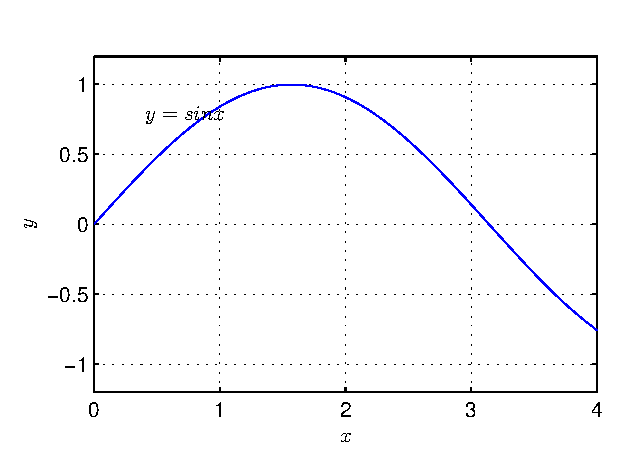
\includegraphics[scale=0.6]{./Pictures/matlabfigchg.eps}
\caption{matlab��ͼ��}
\label{Figmatlab}
\end{figure}

ͼ \ref{Figmatlab} ����ͼΪmatlab���ɵ�epsͼ����ͼΪ����ͼ�е�s1��
�ݺ��������滻���ͼƬ�����԰���һҳ�Ŵ󼸱�������ͼƬ��Ȼ�dz�������
�����ʸ��ͼ�����ơ�
�滻��������������ij��֣���Ϊdvips������cjk�����ݣ�
������ģ���tex-dvi-pdf���ɷ�ʽ���������ں���dvips���̣�ʹ��dvips��ʹ��cct��ʽ��
������ο�CTeX FAQ������ϸ���ӡ�

\subsection{��ͼ��ʹ��}
��Щʱ��������Ҫʹ��һ��ͼ�ŵ�һ����ͼ�У���ΰ汾Ҳ�ṩ����֧�֣�����ʵ�ִ������£�

{
\linespread{1}
\zihao{-5}\noindent
\begin{verbatim}
\begin{figure}[htb]
	\small
	%\centering
	\subfigure[��ͼ1]{
		\begin{minipage}[b]{0.5\textwidth}
			\centering
			\label{fig:SubFigure1} %% label for second subfigure
			\includegraphics[scale=0.6]{./Pictures/matlabfig.eps}
		\end{minipage}}
		\subfigure[��ͼ2]{
			\begin{minipage}[b]{0.5\textwidth}
				\centering
				\label{fig:SubFigure2} %% label for second subfigure
				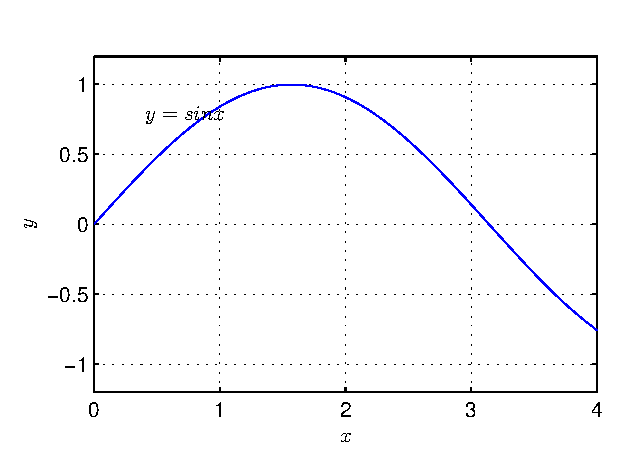
\includegraphics[scale=0.6]{./Pictures/matlabfigchg.eps}
			\end{minipage}}
			\caption{������ͼʾ��}
			\label{Fig:SubFigures}
		\end{figure}
\end{verbatim}
}
ʵ��Ч����ͼ\ref{Fig:SubFigures}��ʾ��

\begin{figure}[htb]
	\small
	%\centering
	\subfigure[��ͼ1]{
		\begin{minipage}[b]{0.5\textwidth}
			\centering
			\label{fig:SubFigure1} %% label for second subfigure
			\includegraphics[scale=0.6]{./Pictures/matlabfig.eps}
		\end{minipage}}
	\subfigure[��ͼ2]{
		\begin{minipage}[b]{0.5\textwidth}
			\centering
			\label{fig:SubFigure2} %% label for second subfigure
			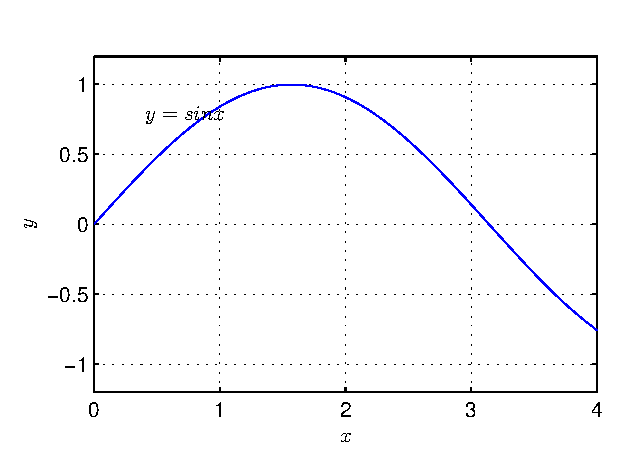
\includegraphics[scale=0.6]{./Pictures/matlabfigchg.eps}
		\end{minipage}}
		\caption{������ͼʾ��}
		\label{Fig:SubFigures}
\end{figure}

\section{�������}

\LaTeX �н��������Word�Ը���һЩ��������ĸ�ʽ������Ч����Word�򵥵öࡣ

\subsection{��ͨ����IJ���}

һ����ͨ�IJ���������������ʾ�������ɵı������ \ref{Tabkeyword} ��ʾ��

{
\linespread{1}
\zihao{-5}\noindent
\begin{verbatim}
{
\begin{table}[htb]
\zihao{5}
\caption{�������}
\label{Tabkeyword}
\centering
\begin{tabular}[t]{c|l|r|p{4cm}}
\hline
���� & ���� & ���� & �����4cm\\
\hline
Center & Left & Right & Width=4cm\\
\hline
\end{tabular}
\end{table}
}
\end{verbatim}
}

\begin{table}[htb]
\zihao{5}
\caption{�������}
\label{Tabkeyword}
\centering
\begin{tabular}[t]{c|l|r|p{4cm}}
\hline
���� & ���� & ���� & �����4cm\\
\hline
Center & Left & Right & Width=4cm\\
\hline
\end{tabular}
\end{table}

�����ʹ��һ������ͼƬ�����ƣ����翪ʼ�����\verb+\begin{table}[htb]+��
�Լ����������\verb+\end{table}+����ͼƬ�����ȣ����˰ѡ�figure��������
��table������������ͬ�����ĺ���Ҳ��ͬ��

\verb+\zihao{5}+�ǰѱ�����ֺŸ�Сһ�ţ�һ����ԣ������ֺ�Ӧ�������ֺ�Сһ�ţ�
�����е������ֺ���С�ĺţ���ô�����е��ֺž�Ӧ����������塣�������һ��Ҫд��
\verb+\begin{table}+ ���·����ܶԸñ��������á�

\verb+\caption{�������}+�DZ���ı��⣬��ͼƬ�����ʽ��ͬ��
���Զ��ӵ�����Ŀ¼��ȥ������������̫����������
\verb+\caption[Ŀ¼�еı���]{�����еı������}+������ʽ��

\verb+label{Tablekeyword}+��ͼƬ�ı�ǩ��ͬ��ֻҪ��������ʹ��\\
\verb+\ref{Tablekeyword}+ �Ϳ��������ɵ��ĵ�����ʾ�����ı�ţ�
ͬ��������ǰ��Ҫ����һ���ո񣬲��ұ�ǩ����ʹ�������ַ���

\verb+\centering+ ʹ����������з��á�

\verb+\begin{tabular}[t]{c|l|r|p{4cm}}+�DZ���ʼ�ı�־��ע����
\verb+\begin+ \verb+{table}+��������\verb+[t]+��ʾ���������Ϸ��������ж��뷽ʽ��
�ж����룬�����\verb+[b]+��Ϊ�е׶��룬�����ֶ��뷽ʽ������ʵ�ʲ�������һ�£�
����ѡ��\verb+{c|l|r|p{4cm}}+��������������е�
���뷽ʽ��cΪ���У�lΪ����룬rΪ�Ҷ��룬p\{4cm\}Ϊ���п���Ϊ4cm����������롣
�м�����ߡ�\verb+|+�����ʾ����ʹ�����ָ��ߣ����û��������߷��ţ���Ӧλ�þ�û�зָ��ߣ�
����� \ref{Tabkeyword} ��û������ߺ����ұߵ����ߡ����дΪ\verb+{|c|l|r|p{10cm}|}+��
��������ߺ����ұߵ������ˡ�
�������Ҫ���ָ��ߣ���дΪ\verb+{clrp{10cm}}+
���ɡ�Ҫʹ��˫���߷ָ��ߣ���дΪ\verb+{c||c}+��������ʹ�������������棬
���籾ģ�������ҳ�������˼����ίԱ����Ϣ�������õı�����ʽ�����ķָ�����ð�š�������
��Ӧ���������\verb+{c@{��}c}+����\verb+@{��}+��

\verb+\hline+���ǻ�һ�����ߣ����û��д��һ�������ῴ������û�к�ָ��ߡ�

����������һ��һ������ģ�ÿһ�н���ʹ�ö��з�\verb+\\+��
ͬһ���в�ͬ�е�Ԫ����\&���ֿ���

\verb+\end{tabular}+��ʾ���������

\subsection{�ѱ��񻻸���ʽ}

��һС�ڽ��ܵķ������ɵı���һ������¿������ˣ�
��\LaTeX ��������ֹ��������һ���������
��������������booktabs-de\index{booktabs-de}��չ�����ñ���������professionalһЩ��
�����չ���ĵ����Ѿ������˱�ģ�����ˣ�ʹ�ñ�ģ�����ֱ��ʹ�����ָ�ʽ��
���������� \ref{Tab3Line} ��ʾ��

{
\linespread{1}
\begin{table}[htb]
\zihao{5}
\caption{��ϸ�߱���ʾ��}
\label{Tab3Line}
\centering
\begin{tabular}[b]{cccc}
\toprule
�� & �� & �� & ����\\
(m) & (cm) & (mm) & (kg)\\
\toprule
1.234 & 5.676 & 332.876 & 3498.5\\
\midrule
548.4 & 23.43 & 34.98 & 923.8\\
\bottomrule
\end{tabular}
\end{table}
}

�� \ref{Tab3Line} ��ʵ�ִ���������ʾ��

{
\linespread{1}
\zihao{-5}\noindent
\begin{verbatim}
{
\linespread{1}
\begin{table}[htb]
\zihao{5}
\caption{��ϸ�߱���ʾ��}
\label{Tab3Line}
\centering
\begin{tabular}[b]{cccc}
\toprule
�� & �� & �� & ����\\
(m) & (cm) & (mm) & (kg)\\
\toprule
1.234 & 5.676 & 332.876 & 3498.5\\
\midrule
548.4 & 23.43 & 34.98 & 923.8\\
\bottomrule
\end{tabular}
\end{table}
}
\end{verbatim}
}

�Ƚ���һ���ⲿ�ִ���Ϊʲô����һ�Դ�����\{\}������������
���Ҫ��������һ�������ݵĸ�ʽ���������ֲ���Ӱ�쵽�������֣�
��ʹ��һ�Դ����Ű�Ҫ������ʽ�IJ�����������
����Ҫ�����ĸ�ʽ���оࡣ�����ĵ�Ĭ���о���1.5���о�
\footnote{ģ���е��о����������$\backslash$linespread\{1.5\}��
��������ֱ�ӵ�1.5�������и����㣬����Ȥ��ͬѧ���Բ鿴�ο�����\cite{LaTeXshzh}}��
������Ҫ�������ɵ����о����������ʽ�űȽ����ۣ�
��˾�����ǰʹ��\verb+\linespread{1}+����������о����Ϊ�����оࡣ
���ھֲ���ʽ�������ں���ġ��ص��ַ�����Ŀ���ѡ�
һ���л�����ϸ���ܣ�����ֻ��ǣ�沿������Ҫ˵����

�ⲿ�ִ�������ͨ���������������ں����������\verb+\toprule+��\verb+\bottomrule+
���DZȽϴֵ�������\verb+\midrule+�DZȽ�ϸ��������
���⣬����һ���������������\verb+\cmidrule+��
�������ʹ��������һС��Ҫ������\verb+\cline+���

\subsection{�е�Ԫ��ϲ��ı���}

���񲻿�������һ���һ��ġ����ֱ���������Ҫ���б���ϲ���
�����Ҿ;�һ������ϲ������ӡ�\LaTeX ֱ��֧���кϲ����кϲ�����Ҫ
��չ��multirow\index{multirow}��֧�֣���ģ���Ѿ�������չ��������ȥ����ֱ��ʹ�á�
��� \ref{TabComplex} ��ʾ����

\begin{table}[htp]
\zihao{5}
\caption{���ӱ���ʾ��}
\label{TabComplex}
\centering
\begin{tabular}[t]{|c|c|c|c|c|}
\hline
\multicolumn{2}{|c|}{��ռ������} & ��3�� & ��4�� & ��5��\\
\hline
\multirow{2}*{��ռ������} & �ڶ��е�2�� & �ڶ��е�3�� & \multicolumn{2}{|c|}{\multirow{2}*{��ռ������������}}\\
\cline{2-3}
& �����е�2�� & �����е�3�� & \multicolumn{2}{|c|}{} \\
\hline
\end{tabular}
\end{table}

�� \ref{TabComplex} ��ʵ�ִ������£�

{
\linespread{1}
\zihao{-5}\noindent
\begin{verbatim}
\begin{table}[htp]
\zihao{5}
\caption{���ӱ���ʾ��}
\label{TabComplex}
\centering
\begin{tabular}[t]{|c|c|c|c|c|}
\hline
\multicolumn{2}{|c|}{��ռ������} & ��3�� & ��4�� & ��5��\\
\hline
\multirow{2}*{��ռ������} & �ڶ��е�2�� & �ڶ��е�3�� & \multicolumn{2}{|c|}{\multirow{2}*{��ռ������������}}\\
\cline{2-3}
& �����е�2�� & �����е�3�� & \multicolumn{2}{|c|}{} \\
\hline
\end{tabular}
\end{table}
\end{verbatim}
}

\verb+\multicolumn{2}{|c|}{��������}+���Ǻϲ��е��������2��ʾ�ϲ����У�
��ʽ�����ʾ�ϲ���ĵ�Ԫ����ж����������зָ����ߣ�ע�����зָ���ʱ���ָ��߷���
\verb+|+��Ҫ���ǡ�

\verb+\multirow{2}*{��������}+�Ǻϲ��е��������2��ʾ�ϲ����У�ע���м��*�š�

ע��ͬʱ�ϲ��кϲ���ʱ���������Ƕ�׷�ʽ���Լ��ϲ�������£�����һ���������еı�ʾ��ʽ��
��ϲ���������ʱ�ڶ��е�\verb+\multicolumn{2}{|c|}{}+��

\verb+\cline{2-3}+��������ֻ���ڶ���������У������2,3,5�У���дΪ\verb+\cline{2-3,5}+
\verb+\cmidrule+�÷�ͬ\verb+\cline+��

\subsection{�����߼������ʽ����չ�����}

�����Ҫʵ�ֱ������Ͻ�����б�ߵ���ʽ��
��ʹ��slashbox\index{slashbox}��չ�����ο����Դ������ĵ���

�����ӵı��񣬱���ָ��ÿһ�еĿ��ȣ������Խ�������\cite{LaTeXshzh}����ɣ�
Ҳ���Խ�����չ��array��tabularx�ȣ�����ʵ�ִ���˴���������������Ȥ��ͬѧ�ɲο�����
\cite{LaTeXshzh, Table:Lapo}�Լ���չ���ڰ����ļ���

\section{��ʽ������}

\LaTeX ����֮������Ҫ���þ����Ű���ָ��ӵ���ѧ��ʽ��������ѧ��ʽ���Ű淽����
�ο�����\cite{LaTeXshzh}����һ���µ����������ܸ��ֹ�ʽ�ı༭��
�������͵������д�ˣ�̫���ˣ����ҹ�ʽ�༭��д�����ҵ���ɫ����

\LaTeX �Ĺ�ʽ�༭Ч��Զʤ��Word�еĹ�ʽ�༭�������ң�ʹ��LaTeX��
��ȫ���õ��Ĺ�ʽ�༭���İ汾���⣬��Ϊ�����﹫ʽ�����ô��ı�д�ġ�
�����Ҿ�һ��СС�Ĺ�ʽ������˵����ʽ�ı�д����ţ���ʽ \ref{Equ:exm} ��ʾ��

\begin{equation}
\label{Equ:exm}
c^2=a^2+b^2
\end{equation}

ʵ��ʽ \ref{Equ:exm} �Ĵ���������ʾ��

{
\linespread{1}
\zihao{-5}\noindent
\begin{verbatim}
\begin{equation}
\label{Equ:exm}
c^2=a^2+b^2
\end{equation}
\end{verbatim}
}

\verb+\begin{equation}+��ͼƬ����������ƣ���ͷ����һ��������ʼ���
ֻ������Ĺؼ�����equation\index{equation}��

\verb+label{Equ:exm}+�Ǹ���ʽһ����ţ��Ա����������á��ù�ʽ�����\LaTeX ����
һ�㲻���˹���Ԥ��

\verb+\ref{Equ:exm}+�����������ù�ʽ�����

\section{����}

�����Ƚϼ򵥣�ֻҪ�������������λ�÷�������\\
\verb+\index{������}+��\\
Ȼ���ĺ���������б��оͳ��֡��������������Ŀ������������ҳ�룬
����֧�����ģ�Ӣ���ַ���
��������жദͬ��������������ж�������ǰ���ĸ��˳���г�����
�ܷ���ģ�������������������������������������ȫ���ؿ��������б����¡�

\section{�����}

ǰ����ܲο�����ʱ���ᵽ��ֻҪ׼�����Լ��IJο��������ݿ⣬
�����òο�����ʱֻ��Ҫ����\verb+\cite{tag}+���ܰ���Ӧ�IJο��������ϡ�
�����tag�����ڲο��������ݿ��и��ο����׶���ı�ǩ�����ܺ��������ַ���
������ף����м���Ӣ�Ķ��ŷֿ���\verb+\cite{tag1,tag2}+��
����Ҫ��������˳��\LaTeX �����������һ�С�

����������硰����[1]���XXX���ĸ�ʽ����ʹ�����´��롣

{\noindent\zihao{-5}\verb+����[\citenum{tag}]���+}

��ģ���Ѿ��Ѹ���ο����׵��г���ʽ����ҵ����Ҫ������ã�����Ҫ���޸ġ�

��������˽����ο����׸�ʽ��������Ϣ����ο���չ��natbib\index{natbib}��custom-bib\index{custom-bib}
�Դ��İ����ĵ��������޶��������ĵ�5��Ҳר�Ż�Բο����׵ĸ�ʽУ��������д�ƪ�����ܡ�

\section{��ע}

��Щʱ����Ҫʹ�ý�ע��\LaTeX �Ľ�ע����Ҳ�Ǻܷ���ģ�
ֻҪ������Ҫ��һ����ע�ĵط�������\verb+\footnote{��ע����}+���ɣ�
��ע���ݳ��Ȳ��ޣ���ע���\LaTeX ��������ġ�
��Ҫ���ģ�ֻ��д�������ע�����ݡ�

���ڱ���ӽ�ע������� \ref{ChapsecList} ��ʾЧ���Dz����������鷳һ�㣬��Ҫ�ѱ���Ž�һ��minipage��ȥ��
�ؼ��������£�

{
\linespread{1}
\zihao{-5}\noindent
\begin{verbatim}
\begin{table}
����
\centering
\begin{minipage}[c]{10cm}
\centering
\begin{tabular}
����
\end{tabular}
\end{minipage}
����
\end{table}
\end{verbatim}
}

\verb+\begin{minipage}[c]{10cm}+��ʾ����һ���ڲ����ж���ģ�
����Ϊ10cm��Сҳ�棬�������Ҫ�������ڲ����������ȷ����
���������Ľ�ע�����ۡ�

\section{�ص��ַ�����Ŀ��ʾ}

�е�ʱ����Ҫ��ijЩ������һ����Ŀ��ʾ������ı�������������Ӵ�����
���ʱ������Ҫ����Ҫ�ı��ʽ�IJ�����һ�Դ�����
\footnote{Ҫʹ��Ӣ���ַ��Ĵ�����\{\}}��������
Ȼ����ͷ��д�������ֺ�֮��������������

����һ�λ�����{\bfseries �Ӵ�}��
{\kaishu\bfseries �п��岢�Ӵ�}����{\heiti ����}������{\zihao{3}������}���塣

��һ�仰��ʵ�ִ������£�

{
\linespread{1}
\zihao{-5}\noindent
\verb+����һ�λ�����{\bfseries �Ӵ�}��{\kaishu\bfseries �п��岢�Ӵ�}����{\heiti ����}������{\zihao{3}������}���塣+
}

��\LaTeX �п����õ�������{\songti ����}\verb+\songti+��{\fangsong ����}\verb+\fangsong+��
{\kaishu ����}\verb+\kaishu+��{\heiti ����}\verb+\heiti+��
{\youyuan ��Բ}\verb+\youyuan+��{\lishu ����}\verb+\lishu+���֡��ֺ�������\verb+\zihao{1}+�ֺŴ�
1��-1��2��-2��һֱ��8���֣�ǰ������ű�ʾС���֣�����-4����С�ĺ����塣
7��8�����ֺ�û��С���ֶ�Ӧ��

���ڼӴ���������\verb+\bfseries+����Ӣ���ַ�ֻҪʹ��\verb+\bf+���ɣ�
�����ַ�Ӧʹ��\verb+\bfseries+��

��������Ч�������ã��������ݲμ�CTeX�Դ��İ����ĵ�ctex.pdf��

�����ʹ�ø�������壬����΢���źڣ����������������������Լ����������ļ��������ϼ��ɡ�
CTeX�ṩ���������壬һ��������Ѿ��㹻ʹ�á�





\chapter{一些使用技巧}



\section{软件使用技巧}

如果在生成文档时发生错误,不要惊慌,可以先把生成的文件全部删除再试一次。
就是把除了tex文件外的其它同名文件都删掉。

使用WinEdt编辑tex文件时,如果嫌命令太长打着费劲,试试只输前几个字母然后按
“Ctrl+Enter”键,哈!WinEdt替你把剩下的部分补全了。

遇到问题不要慌,看下方小窗口里提示的出错信息,会有很多提示你错在哪里的。

不同系统下生成的eps可能会有兼容问题,
如本模版中的setroot.eps和rffndb.eps,在xp和windows 7 x64似乎不能通用。
解决方案很简单,
只要用bmeps -p 1 -c setroot.jpg setrooteps重新生成一次即可解决。
rffndb.eps生成命令同setroot.eps。

这个文档我用的是gVim编辑的,gVim自带的自动补全功能比WinEdt更强大,让我在
编写这个文档时省了不少重复工作量。

如果会使用make程序,那么使用Makefile来生成文档更方便一些。

在UTF-8版本中,如果一个命令后紧跟汉字,比如像这样“\verb+songti好的+”,
编译的时候就会报错,处理办法就是在命令后面加一个空格或者一个大括号,就像这样:
“\verb+songti 好的+”或者“\verb+songti{}好的+”

差不多了,就写这几条吧,想起来什么再写。

把另外几个参考文献当引用例子使用一下:专利\cite{WangZL},标准\cite{WangStd},
电子文档\cite{ZLB:1997},期刊文章\cite{LUOZ:2007},
学位论文\cite{wang:2008,wangmt:2008}。

这份文档从规划到完成,历时近20日,也是自己\LaTeX 学习一个总结吧。

\section{推荐的\TeX 准所见所得编辑器}

如果使用\XeTeX ,那么推荐一个强大的所见所得\TeX 准所见所得编辑器 TeXstudio。
该软件的优点有:

\begin{enumerate}
	
	\item{跨平台软件,可在Windows, MacOS,Linux上安装运行}
	
	\item{有中文语言包界面} 
	
	\item{可以在源码与pdf间关联跳跃,实现准“所见即所得”} 
	
\end{enumerate}

将TeXstudio的默认构建命令改为:XeLaTeX,如图\ref{Construct}所示。

\begin{figure}[th]
	\centering
	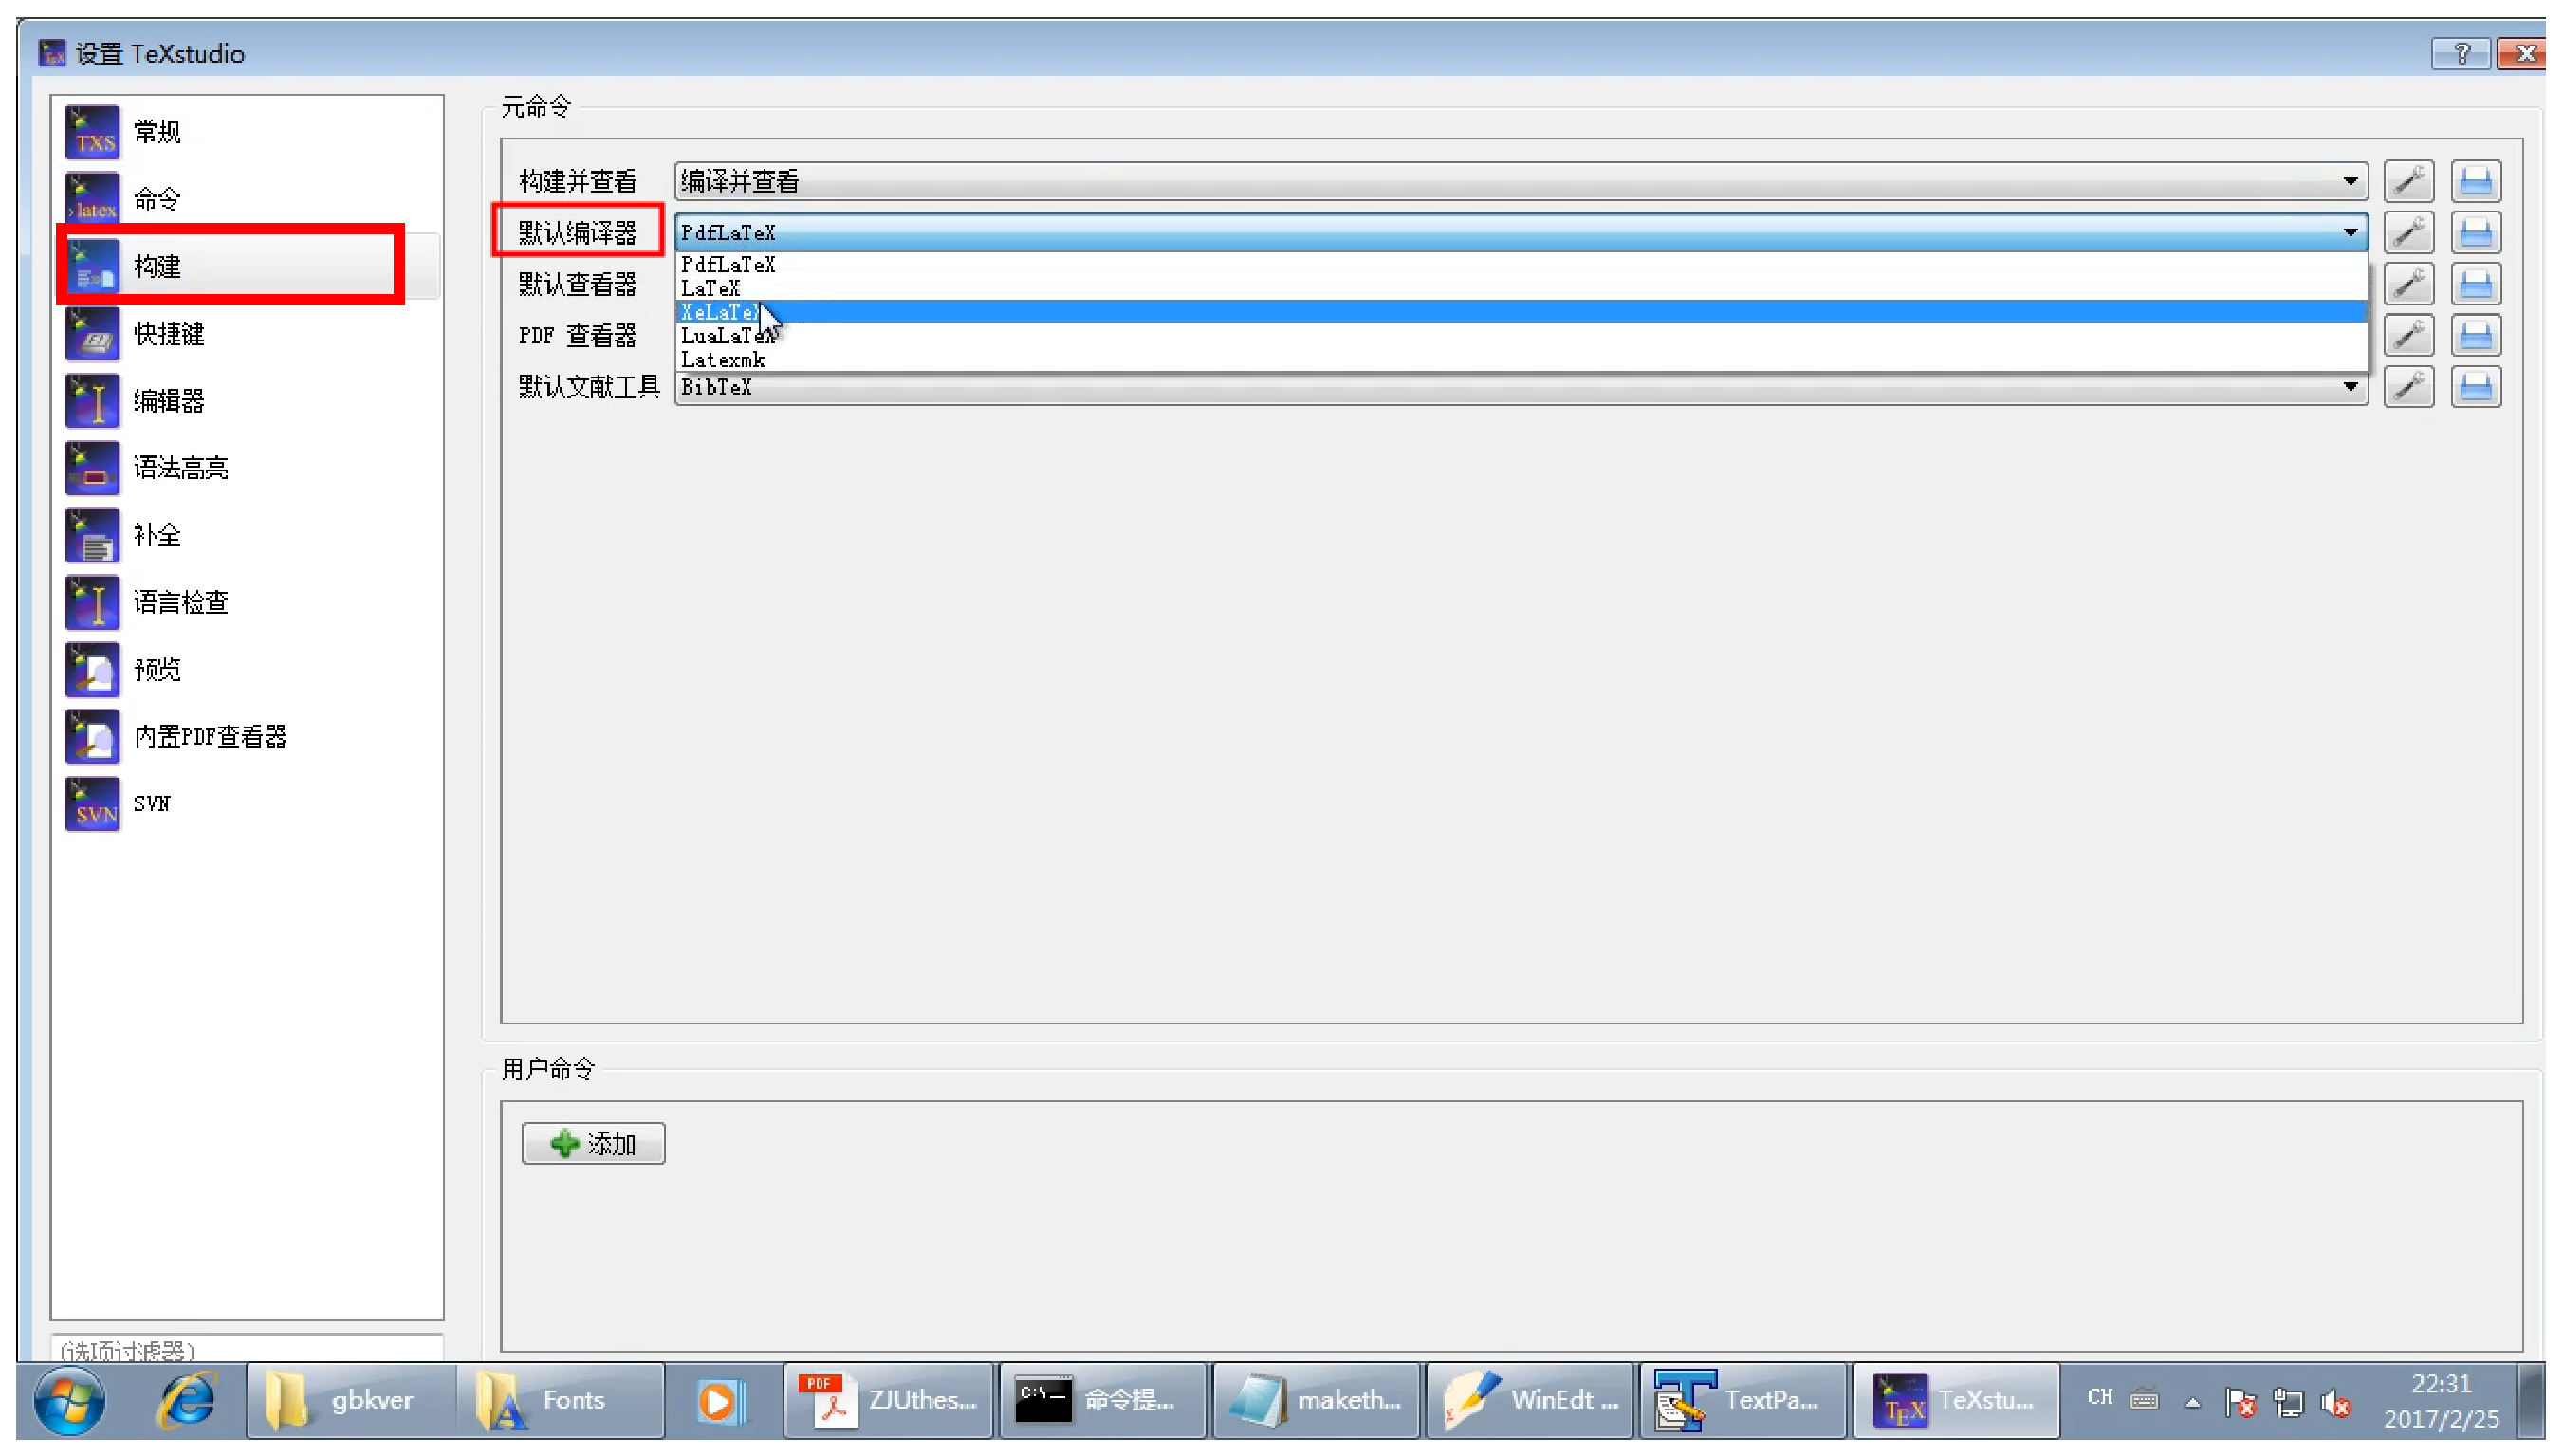
\includegraphics[width=\textwidth]{./Pictures/Construct.eps}\\
	\caption{修改TeXstudio的默认构建命令}
	\label{Construct}
\end{figure}

这样,在使用TeXstudio生成pdf,并打开右侧pdf预览后,就可以使用“Ctrl+鼠标左键”
实现源码与pdf显示之间的来回跳转功能了。

\newpage

从pdf跳转到tex源码,如图\ref{pdftotex}所示。

\begin{figure}[th]
	\centering
	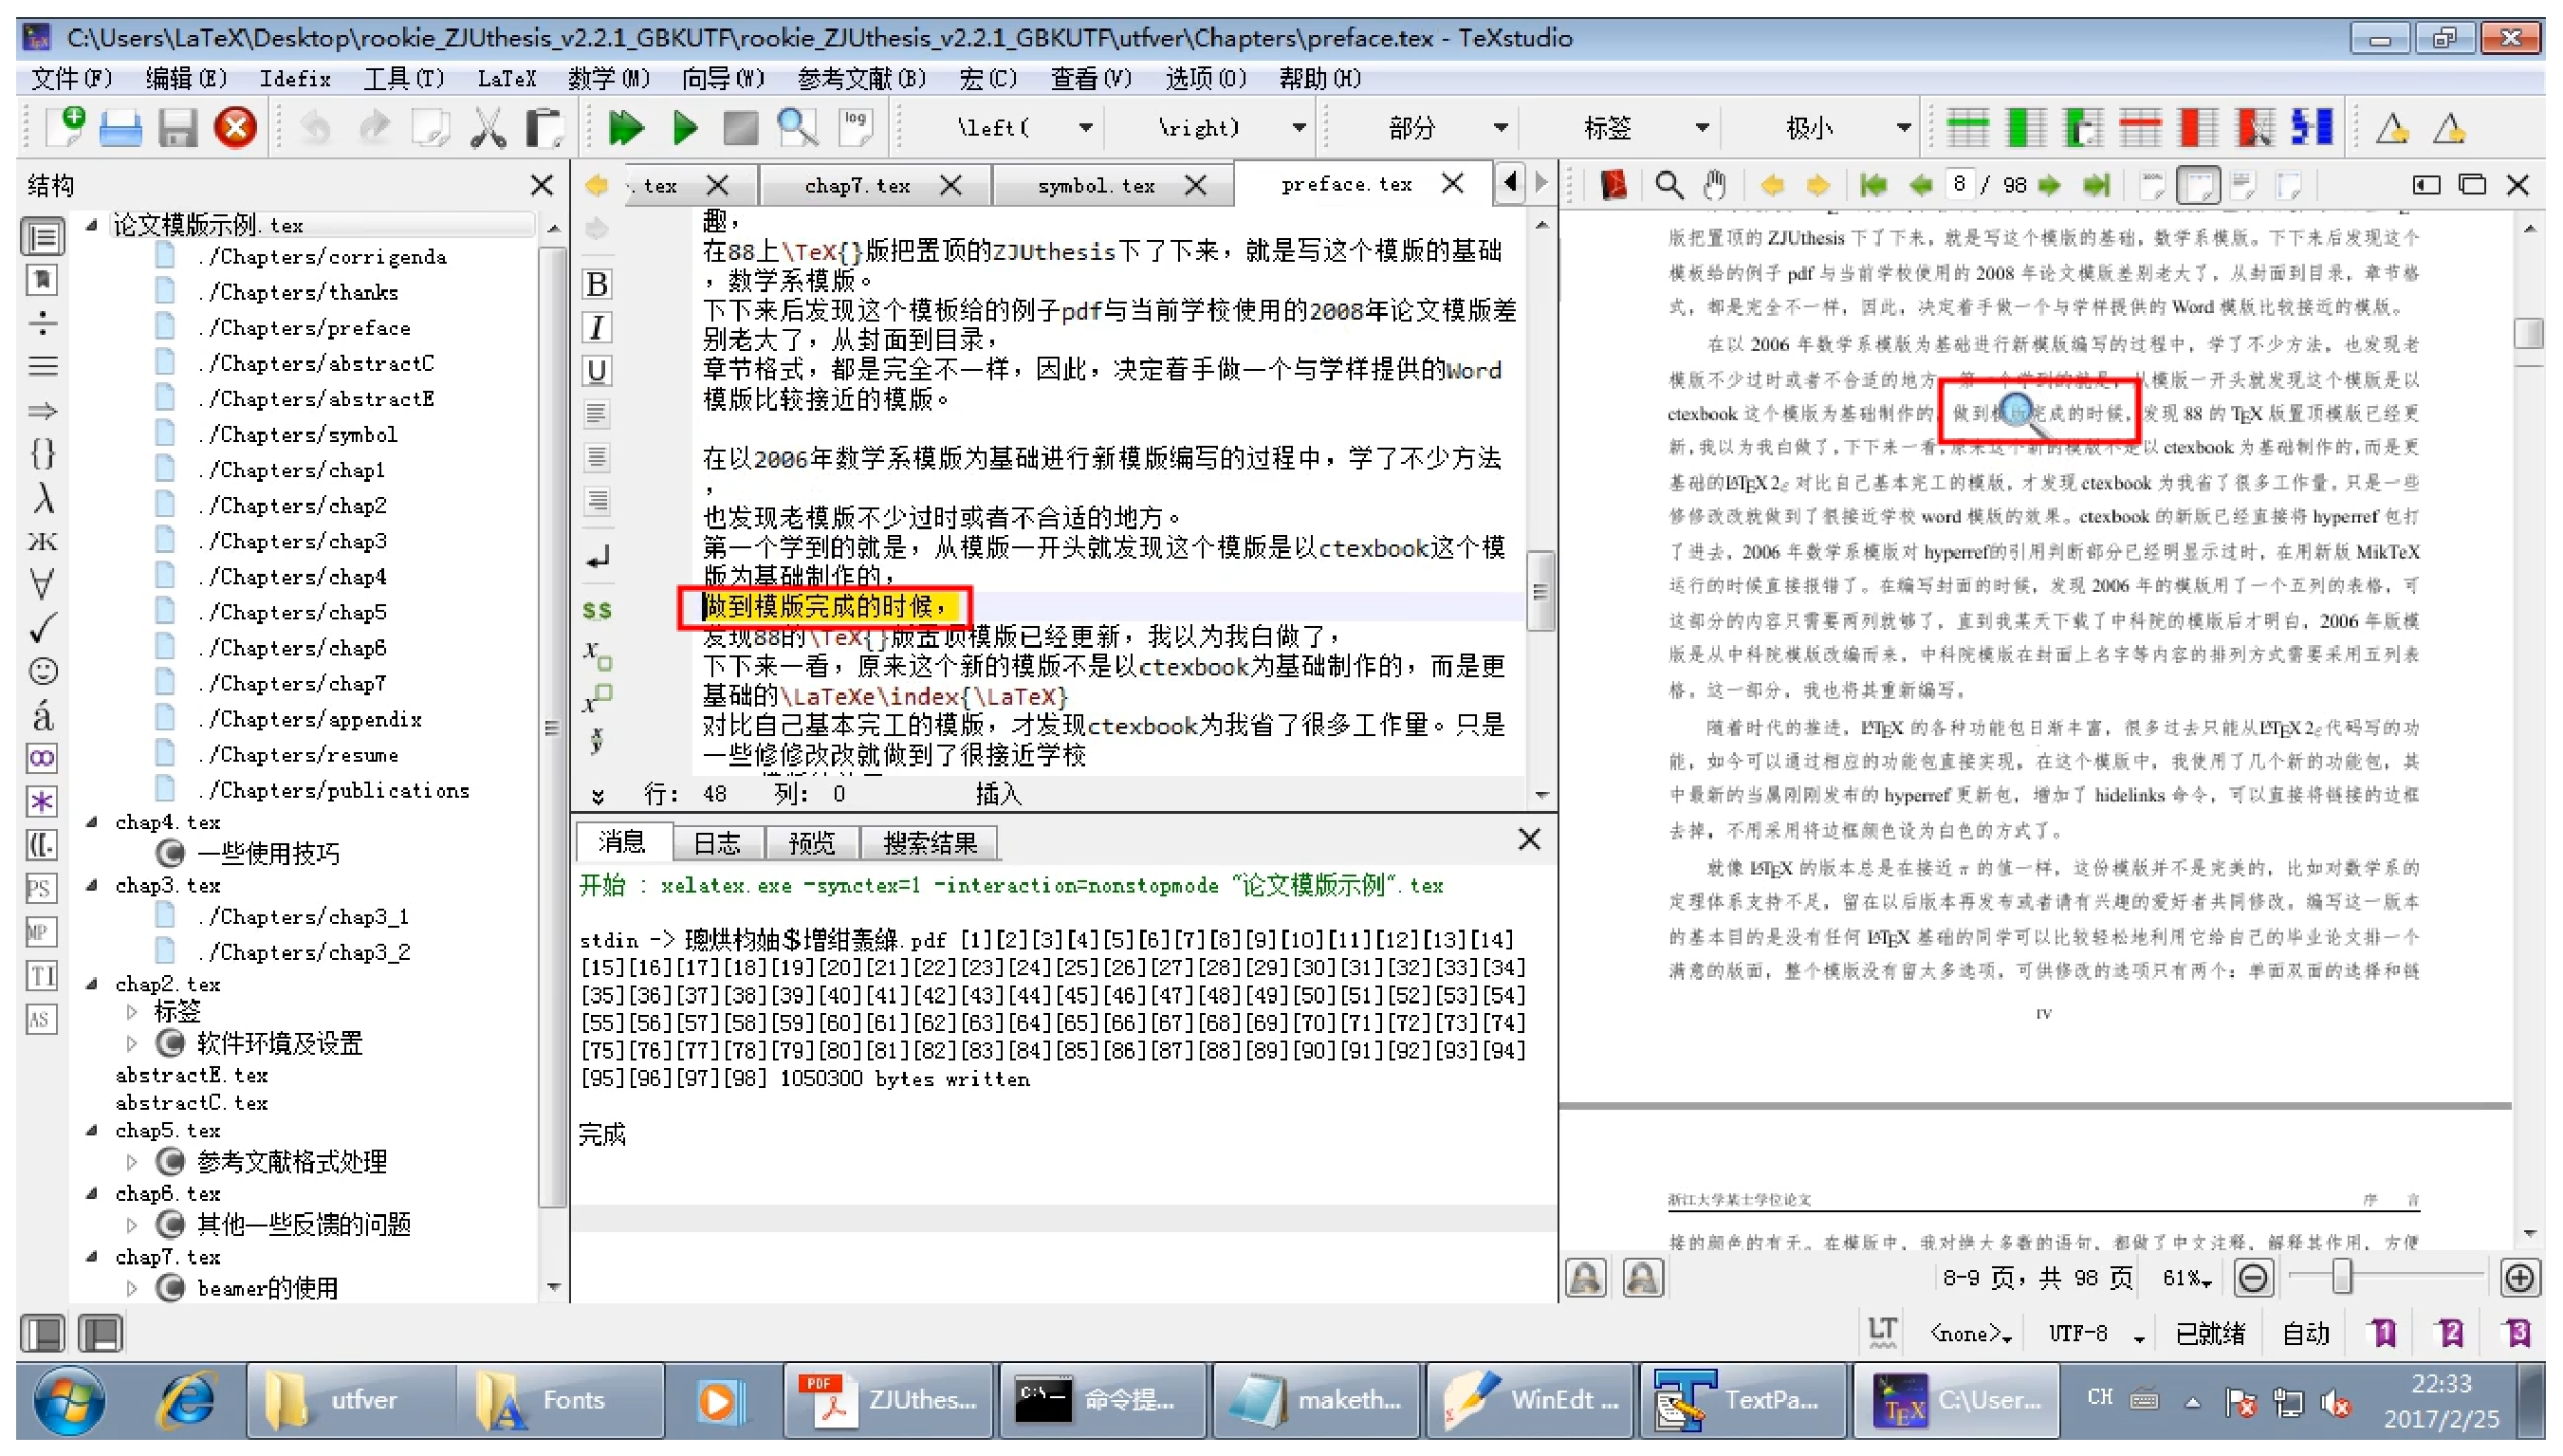
\includegraphics[width=\textwidth]{./Pictures/pdftotex.eps}\\
	\caption{TeXstudio中从pdf跳转到tex源码}
	\label{pdftotex}
\end{figure}

从tex源码跳转到pdf,如图\ref{textopdf}所示。

\begin{figure}[th]
	\centering
	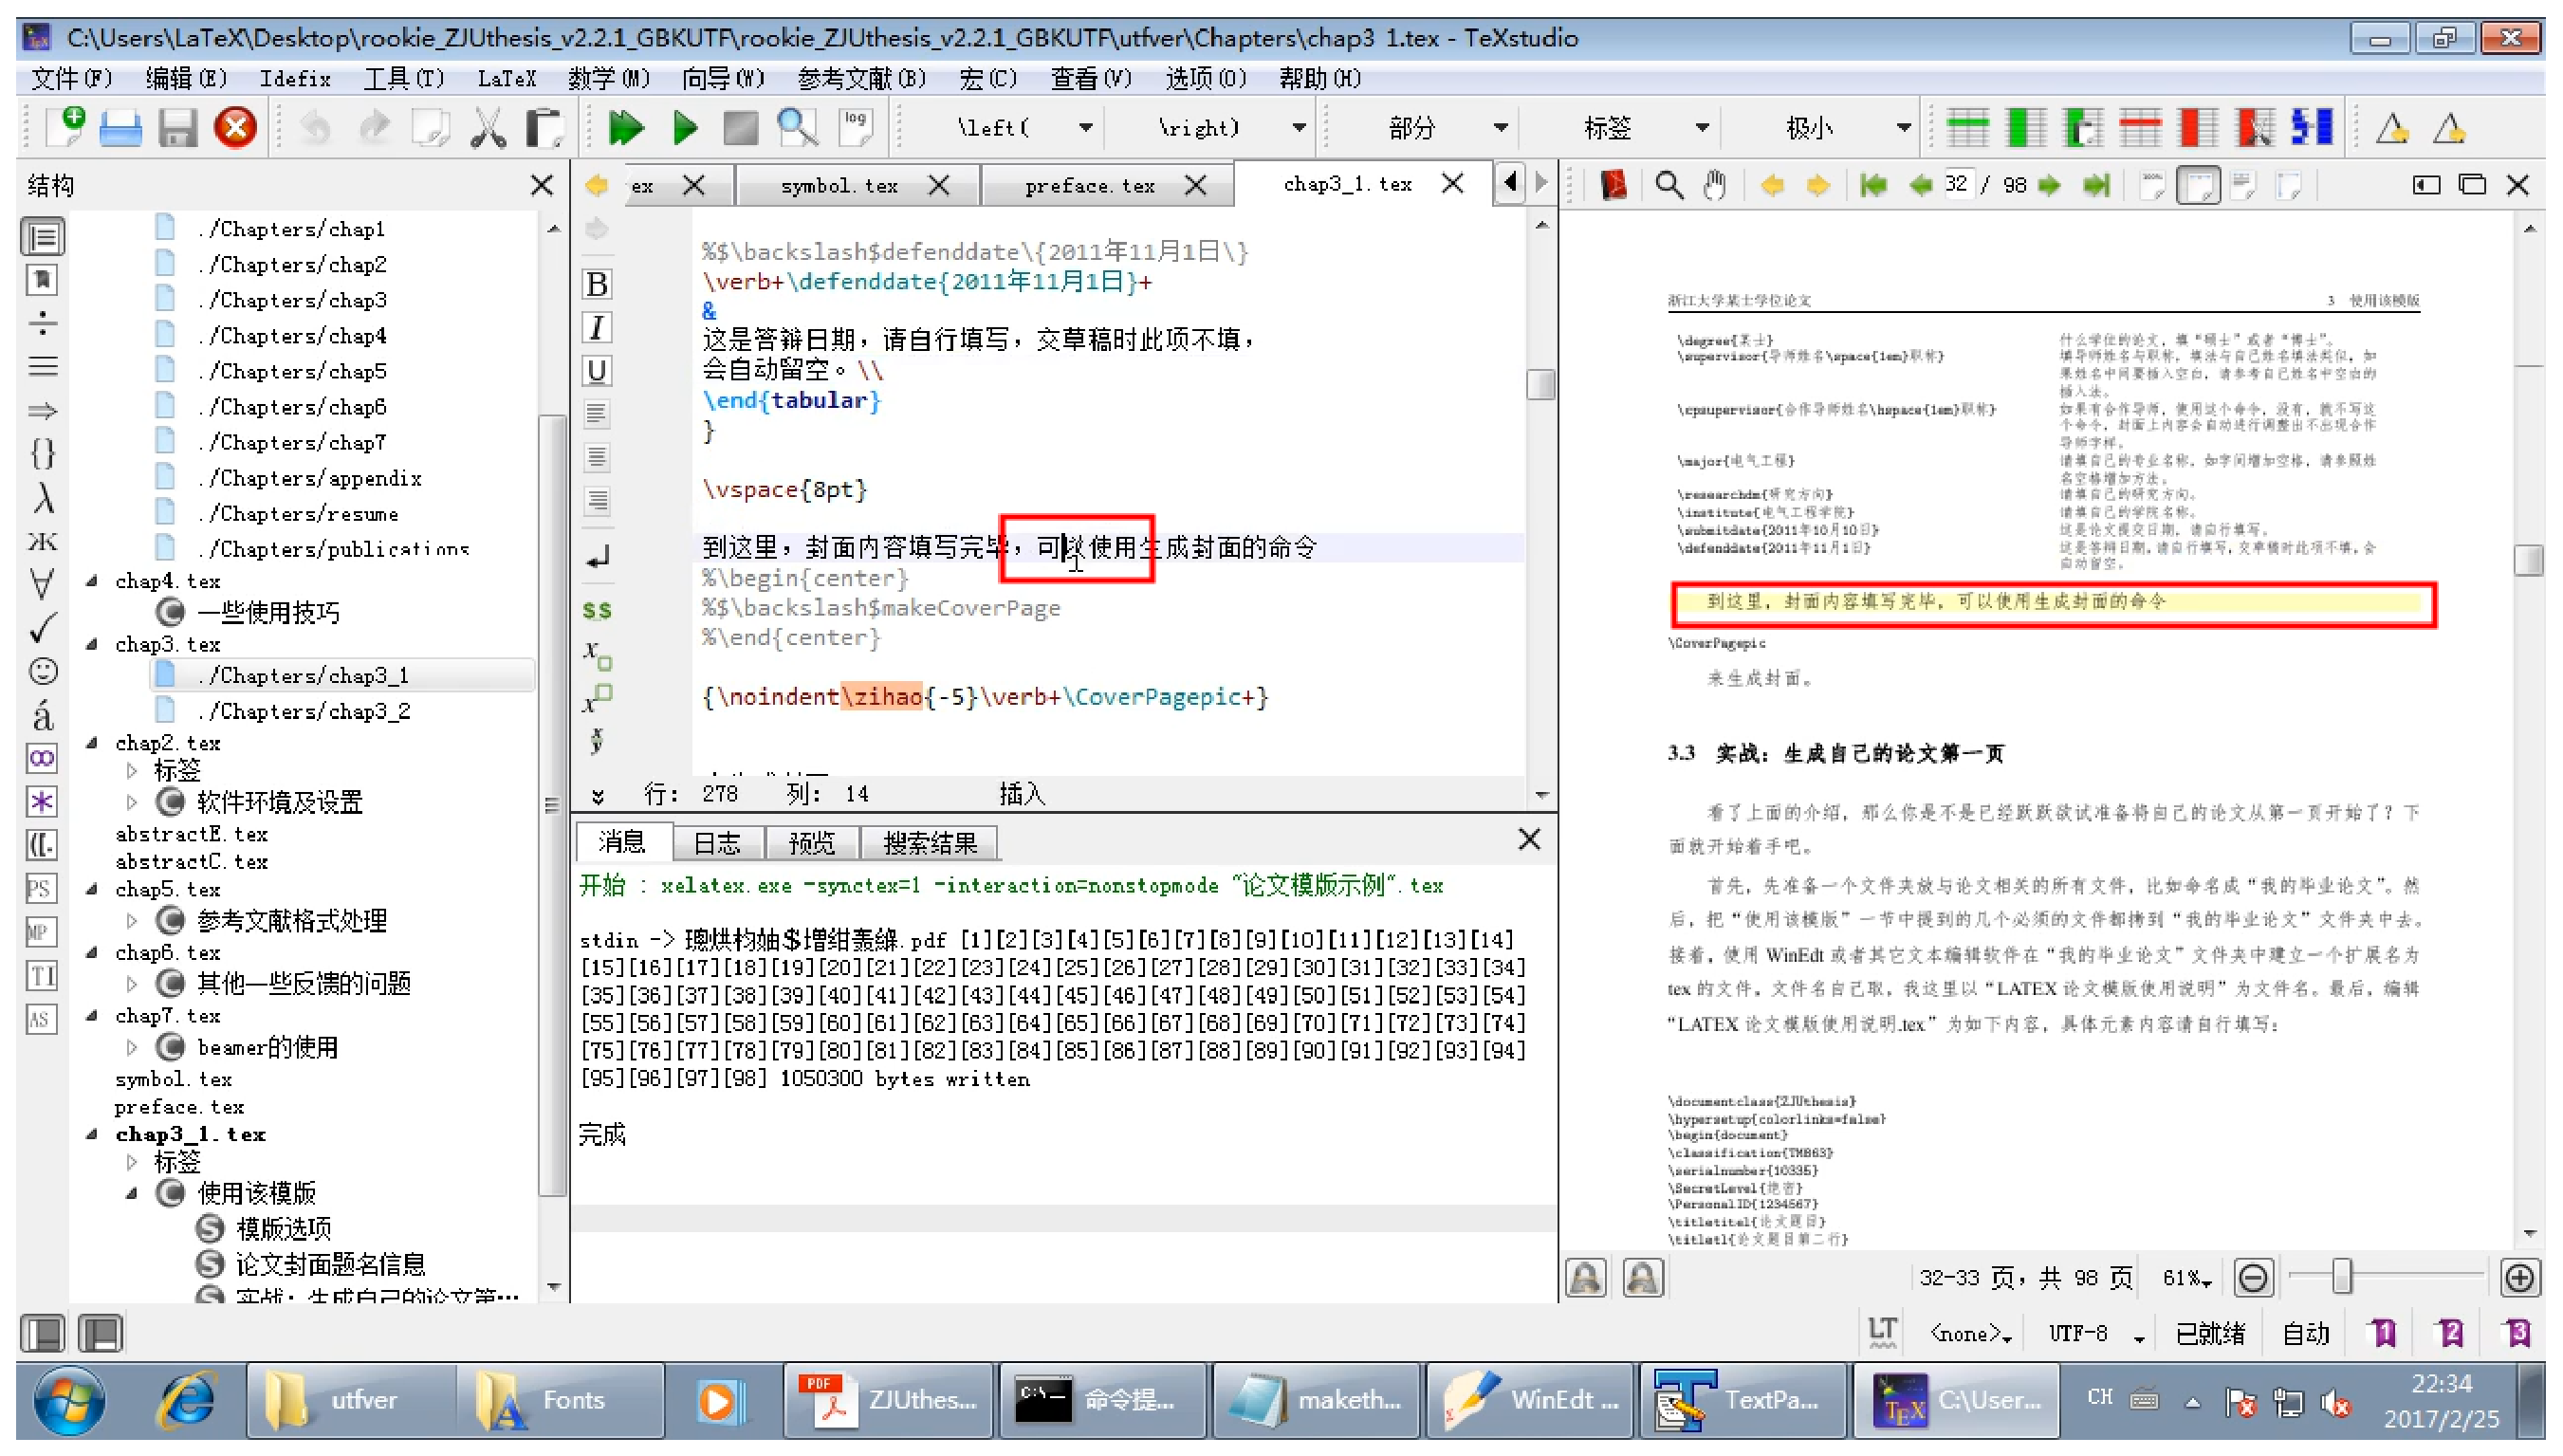
\includegraphics[width=\textwidth]{./Pictures/textopdf.eps}\\
	\caption{TeXstudio中从tex源码跳转到pdf}
	\label{textopdf}
\end{figure}

\chapter{参考文献格式处理}

参考文献是学位论文中重要的一部分,
规范、整齐的参考文献引用格式,对毕业论文质量有重要的影响。

\LaTeX{}提供了一套比较全面的参考文献辅助系统,
涉及参考文献引用格式、文后列写格式两大方面,
其中引用格式又细分为按序号、按人名年代,按人名字母顺序等几小类索引方式,
文后列写格式除以上所述索引方式外,还牵涉外文人名书写格式、
文献信息排列方式、文献信息条目格式等几方面。
如果应用得当,则\LaTeX{}将成为整理参考文献的顶级帮手,
做出非常漂亮统一的参考文献引用内容。
但是,\LaTeX{}的参考文献引用方法又是网上各种资料薄弱的部分,
除了文献[\citenum{LaTeXshzh}]中提到的方式外,
其它找得到的中文资料廖廖无几,系统介绍其使用方式方法的文献更是几乎没有。
这个模版的第一版中,对参考文献部分只做了非常简单的说明,
只能照着搬来使用,但并不能自主进行自由修改。
这一章以下部分将对\LaTeX{}参考文献系统的使用做一个详细的说明。

\section{一般处理方案}

上面已经说过,关于\LaTeX{}的参考文献系统,主要是参考文献[\citenum{LaTeXshzh}]
中提到了一种最简易的方法。即利用thebibliography环境将参考文献条目一条一条地列出来,
有点类似于在一般在Word中的处理方式
\footnote{用NoteExpress,EndNote软件的另说,\LaTeX{}处理参考文献其实也是跟这类软件类似的思路。},也是在最后面一条一条地把参考文献抄写上去。
而且参考文献信息中各个元素的格式也是在抄写中一条一条写进去。

这种方式的好处是简单易行,适用于比较小的文档,参考文献不超过二十个的文章,
但对于毕业论文这种大工程而言,
这种方式就有些力不从心了。
就需要有一种适合于处理大批量,多类型参考文献的方式与工具。

\section{专业处理方案}

\LaTeX{}系统中提供了BibTeX这样一人专门处理参考文献的工具,
这个工具将人工一条条的罗列变成了机器自动整理格式,自动罗列,
但是,因为参考文献格式多种多样,这个工具的也需要有很广泛的适用性,于是,
它被做得很复杂,以至于除了提供的默认方式外,很少有人知道如何去改动它,调整它的行为方式。

\section{参考资料}

前面已经提到,\LaTeX{}提供了一套比较全面的参考文献辅助系统,
按应用范围分为文中引用格式和文后罗列格式两大部分,
这两大部分{\bfseries{互相独立}},其联接的纽带就是被称为“key”的自定义字符串。

关于这两部分功能使用的资料,介绍文中引用格式的比较多,介绍文后罗列格式的比较少。

\LaTeX{}发行版中自带的参考文档已经把这两个问题做了系统的阐述,
只是文档是英文的,没有中文资料,而且文后罗列功能介绍部分写得又比较晦涩难懂。

文中引用格式部分,参考资料是natbib.pdf\cite{natbibdoc}。
就是natbib功能扩展包的包说明文档。
这份资料的大意是根据文后罗列的条目内容,在文中引用是用数字序号,还是用作者年代的方式。
作者年代这种序号方式其实适用于拉丁字母系文献,对中文文献而言还是数字序号比较适用。
这个模版的中就使用了这个natbib功能包的功能,具体设置可以打开cls文件查看我设置的几个选项,
相关选项含义可以参考该文献。这部分内容比较好理解,难度相对比较低。

文后罗列部分的资料比较复杂,最普通的前面讲的文献[\citenum{LaTeXshzh}]中就有。
而关于BibTeX的使用方式的,则需要以下四个在\LaTeX{}发行包中的帮助文档:
merlin.pdf\cite{merlin},makebst.pdf\cite{makebst},btxhak.pdf\cite{btxhak},btxdoc.pdf\cite{btxdoc}。
其作用介绍如下:

\begin{itemize}
\item merlin.pdf是介绍BibTeX的配置文件可配置选项的;
\item makebst.pdf是介绍BibTeX的配置文件结构构成的;
\item btxhak.pdf是介绍BibTeX配置文件中的逆波兰代码基本语法的;
\item btxdoc.pdf是介绍BibTeX默认支持的参考文献类型及其必要信息结构的。
\end{itemize}

\section{\LaTeX{}参考文献组织思路}

前面也已经提到过,\LaTeX{}把参考文献任务分成了两部分,
一个是文中的引用符号填写任务,
另一个则是文后附带的参考文献信息的罗列部分。
这两部分只有在序号或者说是排序的时候由用户指定的"key"来进行关联指定。
这样一来,程序的任务就比较明确了。

首先,先扫描文中参考文献引用,在相应的参考文献库中找到相对应的“key”的条目,记录下来。
然后,根据扫描文中参考文献的引用结果,将相应的参考文献条目挑出来,
根据其设定的顺序(引用顺序,或者是作者年代顺序),将相对应的参考文件信处条目,
BibTeX按照设定的格式列写出来,再由\LaTeX{}将其写到文后中去。
如果打开这个模版对应的“论文模版示例.bbl“文件,可以看到,
实际上是BibTeX帮你写了一个thebibliography环境,
\LaTeX{}还是按照一般的thebibliography环境方式对其进行调用,写入最终生成的pdf文档中去。
也就是说BibTeX这里充当了一个有规则的抄写员的作用。

\section{如何让BibTeX按你的想法干活}

如果文后面的参考文献列表不是自己采用thebibliography环境生成,
那就是是由BibTeX来生成的,
BibTeX生成这样一个参考文献列表的基础信息来自提供的*.bib文件,
这里面用通用的格式写出了各条参考文献的信息,如作者,题名,年代,出版者,出版地等,
也标明了各条参考文献的类型,如期刊文章(article),书籍(book),电子出版物(EPublication)等。
有了这些信息,还需要告诉BibTeX要求输出的格式,BibTeX才能按照要求写出条目。
那么问题就是:如何告诉BibTeX这些格式信息呢?

答案就是*.bst文件,这个文件就是BibTeX的配置文件,它告诉了BibTeX对各种文献类型,文献信息的处理方式。
但这个文件是整个参考文献系统中最复杂也是最核心的部分,
我在这上面花了很长的时候摸索才找到关键所在。
在写第一版的时候,仅仅是根据从网上找到的很少的英文论坛中的几句话,
硬改出了一个接近于浙江大学学位论文要求的参考文献格式,
在这次的改版中,则完全根据其设定规则,按照其设置方式,进行了修改设定。

\section{关键所在:*.bst文件}

正因为bst文件的规则与内容是整个参考文献系统中最复杂的部分,
因此针对这个问题,降低使用者的难度,
BibTeX的开发者们就提代了一套默认的选项来给我们用。
如自带的plain.bst,natbib包提供的plainnat.bst,abbrvnat.bst,unsrtnat.bst,
一般情况下,不是特别的有要求的,这些默认的bst文件也是勉强够用的。

之所以说是勉强够用,是因为提供这些模版的,都是外国人,
他们的行事方式,文献组织方式终归与中国人有一定的不同。
如文献信息罗列的次序,文献类型的说明,都与中国要求的标准有出入。
根据现行的中华人民共和国国家标准 GB/T 7714-2005 文后参考文献著录规则\cite{bibgb},
国内发行的论文等出版物,都应当依照此标准规定的参考文献格式进行参考文献罗列。
国外的默认文献格式当然与国标要求的格式不符,
那么作为患有严重强迫症的模版作者我来说,这些问题当然一定要解决的。

\subsection{bst文件的结构}

既然如此,就来看一下bst文件究竟是一个什么样的内容。
bst文件是一个纯文本文件,可以直接用任何的文本编辑器打开。
最前面是一些注释,bst文件生成时的注释,如这个模版用的ZJUthesis.bst文件开头的注释就说明了
这个bst文件是根据mbsfile\_wdj\_v1.0.mbs这个文件生成了,关于mbs文件的作用将在后面介绍。

{
\linespread{1}
\zihao{-5}\noindent
\begin{verbatim}
mbsfile_wdj_v1.0.mbs  (with options: `seq-no,ed-au,dt-jnl,jttl-rm,pp-last,num-xser,btit-rm,
bt-rm,bkpg-x,gb-fmt,pre-edn,isbn,issn,doi,pp,xedn,no-auword,xand,nfss,')
\end{verbatim}
}

开头的这一段注释说明了这个bst文件的生成配置为seq-no, ed-au, dt-jnl, jttl-rm, pp-last, num-xser, btit-rm, bt-rm, bkpg-x, gb-fmt, pre-edn, isbn, issn, doi, pp, xedn, no-auword, xand, nfss,
这一长串配置选项的具体含义可以在merlin.pdf中查到,
如seq-no代表的含义是文后的参考文献是按文中的引用顺序是行排序的,
如果没有这个选项,就会按照作者名字的字母顺序进行排序。
gb-fmt和no-auword是两个针对该模版增加的两个选项,在merlin.pdf中是没有的,
用来控制输出文献类型标志符,
如期刊文章类型标志符[J],书籍的为[M]等,输出标志符在\LaTeX{}提供的模版中,是没有这个功能的,
是由我在这个模版中添加进去的。
gb-fmt是用于设置按国标[\citenum{bibgb}]格式生成参考文献列表时采用国标格式的选项。
这些设置选项是如何起作用的将在后面的内容中介绍到。

接下来就进入到bst文件的正题部分了,
首先是一个有几十个项的列表,这个列表代表了在这个bst文件中用到的所有代指量名,
如author,title,year等,
这个列表可以根据*.bib参考文献信息库中的文档情况进行自由添加。

再接下来就是一堆的FUNCTION了,很长,
这些FUNCTION就是BibTeX进行文献列表生成时用的程序,
要控制BibTeX的行为,就是要修改这些FUNCTION。
这些FUNCTION是有层次的,在前面的是一些基本的子程序,
到后面,就是由这些子程序构成的复杂功能的大程序。
再到最后,就看到以article,book,proceedings,phdthesis等等
文献类型命名的最终FUNCTION了,
没错,就是这些FUNCTION直接决定了每种文献类型的输出格式。

然后,就没有然后了,这个bst文件就结束了。

\subsection{BibTeX编程的规则}

前面已经讲到,控制BibTeX这个程序的行为就是靠bst文件中列出的FUNCTION,
这些FUNCTION的结构很像一个C语言文件,子程序在前,调用这些子程序的程序在后,
但是这些程序的语法不是C语言语法,而是人读起来比较费劲的逆波兰表示法。

关于逆波兰表示法,我这儿抄一段wiki百科的资料列下。

\begin{description}
\item[逆波兰表示法]
逆波兰表示法(Reverse Polish notation,RPN,或逆波兰记法),是一种是由波兰数学家扬·武卡谢维奇1920年引入的数学表达式方式,在逆波兰记法中,所有操作符置于操作数的后面,因此也被称为后缀表示法。逆波兰记法不需要括号来标识操作符的优先级。

逆波兰结构由弗里德里希·鲍尔(Friedrich L. Bauer)和艾兹格·迪科斯彻在1960年代早期提议用于表达式求值,以利用堆栈结构和减少计算机内存访问。逆波兰记法和相应的算法由澳大利亚哲学家、计算机学家查尔斯·汉布林(Charles Hamblin)在1960年代中期扩充。

在1960和1970年代,逆波兰记法广泛地被用于台式计算器,因此也在普通公众(工程、商业和金融领域)中使用。
\end{description}

正是由于有这么一段现在在少有人使用的表达方式,使得bst文件中的FUNCTION有如天书,
没有足够资料引导的话,很难读懂,也就很难调整使用。

逆波兰表示法的最大特点就是始终在操作一个栈,操作无非压栈出栈,
那么这个BibTeX实际在操作中也是这样,把参考文献信息一个个压入堆栈,
再在适当的时候释放出来,我这里以一个比较简单的standard也就是标准的参考文献类型的FUNCTION代码来解释一下这个BibTeX是具体如何工作的。


{
\linespread{1}
\zihao{-5}\noindent
\begin{verbatim}
FUNCTION {standard}
{
  output.bibitem
  format.authors "author" output.check
  new.block
  format.btitle
  "title" output.check
  "[S]" *
  new.block
  address "address" bibinfo.check
  ":" *
  publisher "publisher" bibinfo.warn * output
  format.date "year" output.check
  fin.entry
}
\end{verbatim}
}

我们来先看第一句FUNCTION {standard},
这一句代表了这个FUNCTION是用来处理standard这样一类参考文献的,
如果被引用的参考文献在库中开头指明是standard类型,那么其相应的在*.bbl文件中的条目,
就由这个函数来进行书写。

这个FUNCTION的函数体第一句 output.bibitem,
这个实际是一个子函数,在bst文件中向前寻找,会很容易找到这个FUNCTION {output.bibitem}的定义。
这里先不具体介绍该子函数的具体细节实现,
其功能就是,在*.bbl文件中写下“$\backslash$bibitem{key}”这样一句,
这里面的"key"代表相应参考文献引用的关键字。
然后在堆栈里压入一个空的字符串,相应的堆栈内容变为:

\begin{center}
\zihao{-5}
\begin{tabular}{r|c|}
第二栈 &\\
\cline{2-2}
第一栈 & 一个空字符串\\
\cline{2-2}
\end{tabular}
\end{center}


*.bbl的内容如下:
\begin{center}
\framebox{
\zihao{-5}
\begin{minipage}{0.6\textwidth}
\vspace{2ex} 
$\backslash$bibitem\{key\}
\vspace{2ex}
\end{minipage}
}
\end{center}

函数体第二句format.authors,
这一句是将这个参考文献中的author部分进行一个格式化,
格式化完毕后,把这个结果压到堆栈里去,
于是乎,这时候,堆栈里出现了第二个元素。

\begin{center}
\zihao{-5}
\begin{tabular}{r|c|}
第三栈 &\\
\cline{2-2}
第二栈 & 作者名字\\
\cline{2-2}
第一栈 & 一个空字符串\\
\cline{2-2}
\end{tabular}
\end{center}

对于中文名字来说,基本用不着怎样的格式化,
怎样的写法都一样,
但对于拉丁字母系人名来说,
可能就会有多种写法,如 John Fitzgerald Kennedy
就可能被写成J.F.Kendey,或者John. F. Kendey,或者
John Kendey等等形式,具体采用哪种形式,在生成bst文件的时候有选项可供选择,
具体选择选项参考merlin.pdf文档,里面有详细的说明。
写到这里,不由得对拉丁语系这种极其蛋疼的姓名体系表示爱莫能助,
在bst文档中,光这种姓名不同的处理方式就占了上百行不止的代码量,
其中各种曲折分支判断,总之,无语了。。。
有一种情况的中文姓名需要处理,就是人名比较多的时候,
在生成bst文件的时候,
有一个选项,“nmlm“选项,用于处理显示几个人名,
后面跟x3,表示最多显示3个名字,跟m3,表示显示3个名字还没显完的时候,加上“et al”这样一个后缀。
另外 “xand“选项用于去掉最后两个中文姓名之间蛋疼地用“and”这个英文词连接,
避免造成的不中不洋的显示情况。

在上面一句的后面,接着了两句:"author" output.check,
为什么说这是两句呢,
\verb+"author"+ 这一句表示将"author"这样一个字符串(不包括引号,下同)压到堆栈里,
这时堆栈里就有两个元素了,最下面的是作者姓名,上面的一个是"author"这个字符串。

\begin{center}
\zihao{-5}
\begin{tabular}{r|c|}
第四栈 &\\
\cline{2-2}
第三栈 & "author"\\
\cline{2-2}
第二栈 & 作者名字\\
\cline{2-2}
第一栈 & 一个空字符串\\
\cline{2-2}
\end{tabular}
\end{center}

然后\verb+output.check+对刚才压入栈的两个元素进行处理,
具体过程为:
首先把"author"弹出来,然后去检查
作者名字是不是一个空的,如果是空的,就会在BibTeX运行时的log里写出
一行警告:"Warning: empty author in cite warning"。
然后再将作者名字下面的空字符串栈输出到*.bbl文件中去,
因为本来就是一个空字符串,所以*.bbl文件在这一步实际上并没有什么变化。

这一步做完,堆栈又成了这个样子了:

\begin{center}
\zihao{-5}
\begin{tabular}{r|c|}
第二栈 &\\
\cline{2-2}
第一栈 & 作者名字\\
\cline{2-2}
\end{tabular}
\end{center}

下面一句\verb+new.block+,
这一句是说明下面一段是新的一句,
一般BibTeX输出的时候会在这一句之前的部分输出一个圆点句号。
比如参考文献中,一般作者名后面跟的就是一个圆点句号。

再下面一句:
\verb+format.btitle+
这一句跟上面的对作者名进行格式化的作用一样,
是将文献题名格式化后,比如字母变成大写之类的,
压入到堆栈中去。
这一句执行完成后,堆栈就变成了:

\begin{center}
\zihao{-5}
\begin{tabular}{r|c|}
第三栈 &\\
\cline{2-2}
第二栈 & 文献题名\\
\cline{2-2}
第一栈 & 作者名字\\
\cline{2-2}
\end{tabular}
\end{center}

下面一句:
\verb+"title" output.check+,
与名字的操作类似,也是检查一下title的的格式是否符合要求,
然后\verb+ouput.check+这一句把{\bfseries{}作者姓名}进行了输出,
这里要注意输出的{\bfseries{}不是文献名称},而是前一个堆栈的内容。
这一句执行后堆栈情况如下:

\begin{center}
\zihao{-5}
\begin{tabular}{r|c|}
第二栈 &\\
\cline{2-2}
第一栈 & 文献题名\\
\cline{2-2}
\end{tabular}
\end{center}

*.bbl的内容如下:
\begin{center}
\framebox{
\zihao{-5}
\begin{minipage}{0.6\textwidth}
\vspace{2ex}
$\backslash$bibitem\{key\}

作者名字.

$\backslash$newblock
\vspace{2ex}
\end{minipage}
}
\end{center}


下面一句\verb+"[S]" *+,其实是两个命令,
\verb+"[S]"+这个命令把字符串"[S]",
压到了堆栈中,这一句执行后的堆栈情况如下:

\begin{center}
\zihao{-5}
\begin{tabular}{r|c|}
第三栈 &\\
\cline{2-2}
第二栈 & “[S]“\\
\cline{2-2}
第一栈 & 文献题名\\
\cline{2-2}
\end{tabular}
\end{center}

\verb+*+这个命令的含义是将堆栈最上面两条弹出来,
把最上面那个跟下面那个合并,再把合并的结果压栈,
这个命令的解释在文献[\citenum{btxhak}]。
于是这个命令执行完后堆栈的情况如下:

\begin{center}
\zihao{-5}
\begin{tabular}{r|c|}
第二栈 &\\
\cline{2-2}
第一栈 & 文献题名[S]\\
\cline{2-2}
\end{tabular}
\end{center}

下一条命令是\verb+new.block+,
这个与上面一样,也是表明文献题后将是一个点句号,
一个block的结束。
这条命令只改变其输出状态,在output.nonnull这个函数中有用。
output.nonnull这个函数后面会讲到,
这里暂时不讲这个函数。

\verb+address "address" bibinfo.check+
这两条命令与前面输入作者,题名类似,也是将出版地格式化一下\footnote{中文出版地没必要去格式化,
英文的地名可能需要格式化,比如全大写之类的。},然后,
对这个信息元素是否存在进行一个判断。
这条命令以后,堆栈的情况变为:

\begin{center}
\zihao{-5}
\begin{tabular}{r|c|}
第三栈 &\\
\cline{2-2}
第二栈 & 出版地\\
\cline{2-2}
第一栈 & 文献题名[S]\\
\cline{2-2}
\end{tabular}
\end{center}

下两句\verb+":" *+
与上面所说的\verb+"[S]" *+
类似,
也是先把":"号压栈,再把它与前面的出版地合起来再压栈,
这两条命令执行后,堆栈情况变为:

\begin{center}
\zihao{-5}
\begin{tabular}{r|c|}
第三栈 &\\
\cline{2-2}
第二栈 & 出版地:\\
\cline{2-2}
第一栈 & 文献题名[S]\\
\cline{2-2}
\end{tabular}
\end{center}

\verb+publisher "publisher" bibinfo.warn * output+
这三句与前面的作用类似,先把出版者格式化一下,
再把它与前面的“出版地:“栈合起来。

这个地方要注意一点的是:
"publisher" bibinfo.warn 这两个命令是检查一下是不是不存在
publisher这个元素,如果不存在,就输出一个警告。

在\verb+output+
命令执行前,堆栈情况为;
\begin{center}
\zihao{-5}
\begin{tabular}{r|c|}
第三栈 &\\
\cline{2-2}
第二栈 & 出版地:出版者\\
\cline{2-2}
第一栈 & 文献题名[S]\\
\cline{2-2}
\end{tabular}
\end{center}

\verb+output+
把第一栈输出,这时候要注意它输出的是文献题名信息。
该条命令执行后,堆栈情况为:
\begin{center}
\zihao{-5}
\begin{tabular}{r|c|}
第二栈 & \\
\cline{2-2}
第一栈 & 出版地:出版者\\
\cline{2-2}
\end{tabular}
\end{center}


*.bbl的内容如下:
\begin{center}
\framebox{
\zihao{-5}
\begin{minipage}{0.6\textwidth}
\vspace{2ex}
$\backslash$bibitem\{key\}

作者名字.

$\backslash$newblock 文献题名[S].

$\backslash$newblock
\vspace{2ex}
\end{minipage}
}
\end{center}


\verb+format.date "year" output.check+
这两条命令与前面类似,将年份压入堆栈。
并把前面出版地:出版者的信息输出到*.bbl文件中去。
这两条命令执行后,堆栈变为:

\begin{center}
\zihao{-5}
\begin{tabular}{r|c|}
第二栈 & \\
\cline{2-2}
第一栈 & 年份\\
\cline{2-2}
\end{tabular}
\end{center}

*.bbl文件的内容如下:
\begin{center}
\framebox{
\zihao{-5}
\begin{minipage}{0.6\textwidth}
\vspace{2ex}
$\backslash$bibitem\{key\}

作者名字.

$\backslash$newblock 文献题名[S].

$\backslash$newblock 出版地:出版者,\footnote{注意这里出版者后面是逗号,不是圆点句号。}

$\backslash$newblock
\vspace{2ex}
\end{minipage}
}
\end{center}

最后一条命令\verb+fin.entry+
把年份输出,堆栈清空,并在*.bbl内容最后面加上圆点句号结束。
*.bbl文件的内容最终如下:
*.bbl文件的内容如下:
\begin{center}
\framebox{
\zihao{-5}
\begin{minipage}{0.6\textwidth}
\vspace{2ex}
$\backslash$bibitem\{key\}

作者名字.

$\backslash$newblock 文献题名[S].

$\backslash$newblock 出版地:出版者,

$\backslash$newblock 年份.
\vspace{2ex}
\end{minipage}
}
\end{center}

这个条目对应出来的参考文献列表格式就是现在看到的文献[\citenum{bibgb}]列出的样子。

这样,一个最简单的标准文献类型的参考文献条目就这样被列了出来。
上面讲都是一些已经成为了模块化的函数,
这些函数最终都是由37条基本命令组合而来的,
这37条基本命令可以在文献[\citenum{btxhak}]中查到。

以下将以上述函数中牵涉的几个命令进行进一步的讲解。

首先看这个函数的第一句:
output.bibitem,
这是一个函数,可以在ZJUthesis.bst文件中找到它的FUNCTION定义:

{
\linespread{1}
\zihao{-5}\noindent
\begin{verbatim}
FUNCTION {output.bibitem}
{ newline$
  "\bibitem{" write$
  cite$ write$
  "}" write$
  newline$
  ""
  before.all 'output.state :=
}
\end{verbatim}
}

下面我们就来逐句解释其含义,

newline\$,这一句含义是在*.bbl文件中新起一行。

"$\backslash$bibitem\{",这一句是将这一个字符串压入堆栈,
这一句执行过后,堆栈就变为:

\begin{center}
\zihao{-5}
\begin{tabular}{r|c|}
第二栈 & \\
\cline{2-2}
第一栈 & "$\backslash$bibitem\{" \\
\cline{2-2}
\end{tabular}
\end{center}

write\$,这一句的作用是将刚写入堆栈的字符串"$\backslash$bibitem\{"写到*.bbl文件中去。

cite\$ write\$,这两句是将引用这条文献的key写到堆栈中去,
然后再将这两句写到*.bbl文件中去。

"\}" write\$,这两句是将后面的大括号写到*.bbl中去。

newline\$,再在*.bbl中另起一行。

"",这一句是将一个空的内容压入堆栈,这个地方的作用后面将会提到。

before.all 'output.state :=,这一句有三个命令,
第一个before.all实际上是一个变量,可以在ZJUthesis.bst文件中找到这样一句:
\#0 'before.all :=,
这说明before.all代表一个整数0。
这个地方要说明的是,在BibTeX中整数的表示方式是加一个\#号。
继续回到这三个命令的解释,先把整数0压入堆栈,
然后'output.state这一句前面的“'”号表示后面跟的是一个变量,
表示将output.state这个变量名而不是变量代表的内容压入堆栈,
最后一个命令,“:=”则是将output.state这个变量赋于整数值0。

再接着往下看第二句
format.authors,这也是一个函数,可以在ZJUthesis.bst中找到如下的函数定义:

{
\linespread{1}
\zihao{-5}\noindent
\begin{verbatim}
FUNCTION {format.authors}
{ author "author" format.names
}
\end{verbatim}
}

可以看出这个函数有三句:
author,这一句把bib文件中的相应的author元素提出压入堆栈,
"author",这一句把“authour”这个字符串压入堆栈,
这个是为了后面的format.names这个函数输出错误信息时提示使用的。
然后后面format.names这个就是对这个作者名字按设定好的格式进行格式化的函数,
在ZJUthesis.bst中也可以找到这个函数,比较长,这里就不再一句一句赘述了。
后面在讲*.mbs文件时这个函数还会被提及到。

好了,对作者名字格式化之后,就该进行输出了,
这里有两句命令,
"author" output.check。
这里又出现了一个"author",这个是给输出时用以错误提示信息用的。
output.check这个函数是重点,在ZJUthesis.bst文件中查询,
可以找到output.check这个函数的定义如下:

{
\linespread{1}
\zihao{-5}\noindent
\begin{verbatim}
FUNCTION {output.check}
{ 't :=
  duplicate$ empty$
    { pop$ "empty " t * " in " * cite$ * warning$ }
    'output.nonnull
  if$
}
\end{verbatim}
}

在运行这个函数之前,堆栈情况如下:

\begin{center}
\zihao{-5}
\begin{tabular}{r|c|}
第四栈 & \\
\cline{2-2}
第三栈 & "author"\\
\cline{2-2}
第二栈 & 作者姓名\\
\cline{2-2}
第一栈 & 一个空字符串 \\
\cline{2-2}
\end{tabular}
\end{center}

第一行包含两个命令:'t :=,
第一个命令't代表将t这个变量名压入堆栈,
在BibTeX中,默认定义了两个字符型变量,s 和 t,
在ZJUthesis.bst文件中可以找到这两个变量的定义:
STRINGS { s t}。
在将t这个变量名压入堆栈后,堆栈变为:

\begin{center}
\zihao{-5}
\begin{tabular}{r|c|}
第五栈 & \\
\cline{2-2}
第四栈 & 't \\
\cline{2-2}
第三栈 & "author"\\
\cline{2-2}
第二栈 & 作者姓名\\
\cline{2-2}
第一栈 & 一个空字符串 \\
\cline{2-2}
\end{tabular}
\end{center}

第二个命令:=,是将堆栈最上面两个弹出,将第二个弹出的值赋到第一个值指向的变量中去。
即将"author"赋给t变量,这个命令执行后,堆栈变为:

\begin{center}
\zihao{-5}
\begin{tabular}{r|c|}
第三栈 & \\
\cline{2-2}
第二栈 & 作者姓名\\
\cline{2-2}
第一栈 & 一个空字符串 \\
\cline{2-2}
\end{tabular}
\end{center}

下一行命令duplicate\$,这个是将堆栈最上面的一个复制一个再压入堆栈,
这个命令执行后,堆栈变为:

\begin{center}
\zihao{-5}
\begin{tabular}{r|c|}
第四栈 & \\
\cline{2-2}
第三栈 & 作者姓名\\
\cline{2-2}
第二栈 & 作者姓名\\
\cline{2-2}
第一栈 & 一个空字符串 \\
\cline{2-2}
\end{tabular}
\end{center}

再下一个命令empty\$,是判断堆栈最上面一个是不是空字符串的。
具体操作过程是,先把最堆栈最上面一个弹出,
判断如果是空,就将1压入堆栈,否则就将0压入堆栈。
如果作者姓名不为空,堆栈就变为:

\begin{center}
\zihao{-5}
\begin{tabular}{r|c|}
第四栈 & \\
\cline{2-2}
第三栈 & 0\\
\cline{2-2}
第二栈 & 作者姓名\\
\cline{2-2}
第一栈 & 一个空字符串 \\
\cline{2-2}
\end{tabular}
\end{center}

下面的一行用大括号括起来了:
\{ pop\$ "empty " t * " in " * cite\$ * warning\$ \}。
用大括号括起来代表把这一样串代码作为一个嵌入的子函数,
然后把这个子函数的入口压入堆栈。
如果执行这个子函数,就是如下一串操作:
把堆栈最上面一个元素弹出,
输出一个字符串,比如:“empty author in citekey”,
看到了吧,这个地方的t就变成了"author",这是前面几句进行的赋值。

\begin{center}
\zihao{-5}
\begin{tabular}{r|c|}
第五栈 & \\
\cline{2-2}
第四栈 & 嵌入子函数的入口\\
\cline{2-2}
第三栈 & 0\\
\cline{2-2}
第二栈 & 作者姓名\\
\cline{2-2}
第一栈 & 一个空字符串 \\
\cline{2-2}
\end{tabular}
\end{center}

下面一行命令'output.nonnull,这个前面的'号还是表示把这个函数的入口压入堆栈,
当然也可以用\{output.nonnull\}。

这一句执行后,堆栈情况如下:

\begin{center}
\zihao{-5}
\begin{tabular}{r|c|}
第六栈 & \\
\cline{2-2}
第五栈 & output.nonnull 函数的入口\\
\cline{2-2}
第四栈 & 嵌入子函数的入口\\
\cline{2-2}
第三栈 & 0\\
\cline{2-2}
第二栈 & 作者姓名\\
\cline{2-2}
第一栈 & 一个空字符串 \\
\cline{2-2}
\end{tabular}
\end{center}

最后一个命令if\$一个比较关键的命令,也是一个常用的命令。
这个命令的操作是将堆栈最上面三个元素弹出,
然后,根据第三个弹出的元素是0还是1进行判断,
如果是0,就执行第一个弹出的元素指向的函数,
如果是1,就执行第二个弹出的元素指向的函数。
这实际上就是一个分支判断函数。
我们来分别来看一下第三栈里是0和是1两种情况的执行结果吧。

弹出三个元素后,堆栈就变为:

\begin{center}
\zihao{-5}
\begin{tabular}{r|c|}
第三栈 & \\
\cline{2-2}
第二栈 & 作者姓名\\
\cline{2-2}
第一栈 & 一个空字符串 \\
\cline{2-2}
\end{tabular}
\end{center}

\begin{enumerate}

\item{}
如果第三个弹出的元素是1,那么就说明作者姓名是个空的字符串,
那么就执行那一长串命令组成的函数:pop\$ "empty " t * " in " * cite\$ * warning\$。
第一个命令,pop\$,把空的作者姓名弹出。堆栈变为:

\begin{center}
\zihao{-5}
\begin{tabular}{r|c|}
第三栈 & \\
\cline{2-2}
第一栈 & 一个空字符串 \\
\cline{2-2}
\end{tabular}
\end{center}

后面的一串就是往堆栈中压入元素,然后再合并,压入,再合并,
到warning\$命令之前,堆栈变为:

\begin{center}
\zihao{-5}
\begin{tabular}{r|c|}
第三栈 & \\
\cline{2-2}
第二栈 & "empty author in citekey"\\
\cline{2-2}
第一栈 & 一个空字符串 \\
\cline{2-2}
\end{tabular}
\end{center}

这里面这个“citekey”指给相应参考文献的别名。
可以看到,这个时候堆栈最上面写了一条警告信息,
那么下面紧跟的命令warning\$就把这条警告信息输出到log文件和输出命令行里去了。

\item{}
如果第三个弹出的元素是0,则表示作者姓名不是空字符串,
这是正常情况,这个时候就执行output.nonnull这个函数,
把作者姓名前面的信息段写入到*.bbl文件中去。
这个地方一定要注意,这时写入的并不是作者姓名这个信息,
而是它下面的第一栈,一个空字符串。
为什么是这样,下面将继续介绍output.nonnull这个函数在做什么。

\end{enumerate}

下面接着向下介绍这个output.nonnull函数。
在执行这个函数之前,堆栈情况如下:

\begin{center}
\zihao{-5}
\begin{tabular}{r|c|}
第三栈 & \\
\cline{2-2}
第二栈 & 作者姓名\\
\cline{2-2}
第一栈 & 一个空字符串 \\
\cline{2-2}
\end{tabular}
\end{center}

output.nonnull函数定义如下:

{
\linespread{1}
\zihao{-5}\noindent
\begin{verbatim}
FUNCTION {output.nonnull}
{ 's :=
  output.state mid.sentence =
    { ", " * write$ }
    { output.state after.block =
        { add.period$ write$
          newline$
          "\newblock " write$
        }
        { output.state before.all =
            'write$
            { add.period$ " " * write$ }
          if$
        }
      if$
      mid.sentence 'output.state :=
    }
  if$
  s
}
\end{verbatim}
}

第一行's :=,这是两个命令,
第一个命令,把s这个变量名放进堆栈,
第二个命令:=,把s变量名弹出,再把作者姓名这个字符串弹出,
把作者姓名这个字符串赋给变量s。
这两个命令完成后,堆栈变为:

\begin{center}
\zihao{-5}
\begin{tabular}{r|c|}
第二栈 & \\
\cline{2-2}
第一栈 & 一个空字符串 \\
\cline{2-2}
\end{tabular}
\end{center}

下面的命令实际是几个嵌套的判断分支,
最外层的分支是这样一个判断:

output.state mid.sentence =,

这一行共三个命令,前两个都是变量,一个是output.state,
另一个是mid.sentence,
从前面已经知道,output.state已经被赋值为before.all,
即一个整数值0,
而mid.sentence的值是1,
第三个命令=号就是判断一下前面两个数值是不是相等的,
结果当然是不等,于是一个0就压进了堆栈之中,
这样,程序就进入了下面的分支:

output.state after.block =

这一句与上面一句类似,也是进行一个判断,
明显,output.state 也不与after.block(值为3)相等,
于是又进入了下面一个分支:

output.state before.all =

这次相等了,于是运行紧挨着它的分支:
这个分支只有一个命令:write\$,
这个命令就是将堆栈中最上面的一个元素写到*.bbl文件中去,
根据此时堆栈的状态,
此时写入*.bbl的只是一个空字符串,也可以说什么也没有写。
*.bbl的内容仍是:

\begin{center}
\framebox{
\zihao{-5}
\begin{minipage}{0.6\textwidth}
\vspace{2ex} 
$\backslash$bibitem\{key\}
\vspace{2ex}
\end{minipage}
}
\end{center}

执行之后的下一句命令

mid.sentence 'output.state :=

把output.state 的值改为mid.sentence(其值为1)

最后一行的一句s,把刚才存进去的作者姓名,
又压回了堆栈,这条命令之后,堆栈内容变为:

\begin{center}
\zihao{-5}
\begin{tabular}{r|c|}
第二栈 & \\
\cline{2-2}
第一栈 & 作者姓名 \\
\cline{2-2}
\end{tabular}
\end{center}

下面让我们回到standard这个类的函数中来,
下一句函数是new.block,
我们找到它的函数定义如下:

{
\linespread{1}
\zihao{-5}\noindent
\begin{verbatim}
FUNCTION {new.block}
{ output.state before.all =
    'skip$
    { after.block 'output.state := }
  if$
}
\end{verbatim}
}

这个函数的操作过程如下,先对output.state 进行判断,
根据上面提到的,现在的output.state的值是mid.sentence,
这里就与before.all不相等了。
于是执行after.block 'output.state :=这一行,
把output.state的值又改为after.block.

接下来的两行命令与前面的比较类似,

format.btitle
”title” output.check

对文献标题进行格式化,然后再进行输出,
但与前面输出不同的时,此时output.state的状态是after.block。
该状态在output.nonnull中对应的运行行是:


{
\linespread{1}
\zihao{-5}\noindent
\begin{verbatim}
          add.period$ write$
          newline$
          "\newblock " write$
\end{verbatim}
}

运行该段命令段前,堆栈的状态是:

\begin{center}
\zihao{-5}
\begin{tabular}{r|c|}
第二栈 & \\
\cline{2-2}
第一栈 & 作者姓名 \\
\cline{2-2}
\end{tabular}
\end{center}

这一段命令行解释如下:
add.period\$是在当前堆栈最上面一个字符串元素后面加一个“.”号,
就是英文句号。
这条命令后,堆栈的状态变为:

\begin{center}
\zihao{-5}
\begin{tabular}{r|c|}
第二栈 & \\
\cline{2-2}
第一栈 & 作者姓名. \\
\cline{2-2}
\end{tabular}
\end{center}

注意“作者姓名”后面紧跟的英文圆点句号。

下一条命令是write\$,就是把堆栈中最上面的元素写到*.bbl中,
这条命令之后,*.bbl的内容变为:

\begin{center}
\framebox{
\zihao{-5}
\begin{minipage}{0.6\textwidth}
\vspace{2ex}
$\backslash$bibitem\{key\}

作者名字.

\vspace{2ex}
\end{minipage}
}
\end{center}

再下面两行命令

newline\$ \\
"$\backslash$newblock" write\$"

则是在*.bbl中重启一行,并写下了 "$\backslash$newblock"这样一个字符串,
这两行命令执行后,*.bbl文件内容如下:

\begin{center}
\framebox{
\zihao{-5}
\begin{minipage}{0.6\textwidth}
\vspace{2ex}
$\backslash$bibitem\{key\}

作者名字.

$\backslash$newblock
\vspace{2ex}
\end{minipage}
}
\end{center}

这一段命令执行后,output.state 再次被修改为 mid.sentence,
并且文献题目被从s变量中再次压回堆栈。
堆栈变为:

\begin{center}
\zihao{-5}
\begin{tabular}{r|c|}
第二栈 & \\
\cline{2-2}
第一栈 & 文献题名 \\
\cline{2-2}
\end{tabular}
\end{center}

其后的函数与上面所述函数作用、结构相同,在后面不再详述。

\subsection{bst文件的调试技巧}

从上面的的bst文件的编程例子可以看出,
BibTeX就是按照操作堆栈以及输出堆栈中字符串的方式,
实现对*.bbl文件的自动编写的。

那么,在掌握了*.bst文件的编程规则之后,
就可以自己编写自己需要的参考文献格式,
那么在编写过程中,自然要不断调试输出的效果以及查找问题所在,
这个时候就需要一些debug的方式来辅助编程。
这一小节将对这些编程中常用的调试方式进行一下介绍。

在调试*.bst文件的输出效果时,
当然不用每次都用一篇文章来一次次试验其输出效果,
大部分时候,只需要运行一次BibTeX这个程序,
再看一下*.bbl中的内容,即可判定该*.bst文件是否符合要求。

如果*.bbl文件中输出的内容不对,
那么就需要查看BibTeX运行中的堆栈情况,
查看堆栈我推荐以下几个命令组合进行查看。

\begin{enumerate}
\item{duplicate\$ top\$}

这两个命令的操作分别是复制堆栈最上面一个元素,
把最上面一个元素弹出并输出其值到BibTeX运行输出命令行中去。
这样,这两个命令的组合实际上就成了运行过程中查看堆栈最上面一个元素的值,
起到了debug中查看当前程序内存状态的作用。

\item{swap\$ duplicate\$ top\$ swap\$}

这个与上面类似,不同的是这个命令用来查看堆栈最上面第二个元素的值。
一般情况下,运行中可能牵涉两个元素的值,
用这个方法与上面的方法结合,就可以实现查看堆栈最上面两个元素值的作用。

\item{stack\$}

这个命令是把堆栈中所有元素一股脑儿全倒出来并显示出来,
一般这个调试方法不太常用。

\item{top\$}

把需要查看的状态量,比如output.state,先压入堆栈,
再用top\$这个命令查看它的值。
注意这里top\$与pop\$命令的区别,前者是将元素弹出后再显示出来,
后者是只弹出,不显示。

\end{enumerate}

一般情况下,对*.bst文件进行调试使用上面几种调试命令就可以了,
将这些命令插入到*.bst文件中的合适位置,
就可以查看*.bst文件在运行中的相应状态。
调试完后,不要忘记将它们从*.bst文件删除。

\section{*.mbs与*.dbj文件}

前面已经讲到,BibTeX这个程序工作设置主要就是参考*.bst文件,
有什么样的*.bst文件,就有什么样的参考文献格式输出。
从而实现了参考文献的自动格式化输出,
当需要改变参考文献的输出格式时,
只需要更换相应的bst文件即可。

但是,从上面一节介绍bst文件的语法规则及使用技巧的情况来看。
bst并不是一个很好用的格式,
它的语法太过晦涩,即便是对其语法特点有较好的理解,
理清各个子函数之间的关联脉络也是一件比较费心思的事。
为了解决这个问题,又出现了更高一级的bst文件配置方案:
mbs文件和dbj文件就是这样一种配置方法。

这里我先不谈mbs文件和dbj文件的内容结构,
先讲一下这种配置方法的基本思路。
既然bst文件是那样晦涩难懂难编写,
那么作为开发者,就先编写一套涵盖大部分人应用的,
比较完整的bst格式输出集,
然后再定一些相对较为简单的选项配置文件,
比如人名要显示几个,文献来源要不要粗体或者斜体处理之类的,
利用这些配置选项,把所需要的bst语句抽出来,
写到*.bst文件中去,这样就生成了我所需要的参考文献格式。
这种思路实际上就类似于人一般做事的思路,
比如一个饭店的厨师,
顾客说要要少放盐,我就放盐的时候,少放一点点,
多放辣椒,就放的时候多放一些,
先煮后炸,或者先炸后煮,
同一道菜,不同顾客不同要求,
在流程中作一些小的改动,就能出很多种花样儿来。

\subsection{一般的bst文件的生成过程}

根据参考文献[\citenum{makebst}]makebst.pdf中的说明,
一般情况下,只需要运行

tex makebst.tex

然后就会有一系列问答式的选项进行回答,
如生成的dbj文件和bst文件的文件名,
这里我用的是dbjfile\_wdj\_1.0和ZJUthesis
其它如显示几个作者名,文献标题是否采用粗体或者斜体等等问题,
回答完之后,就可以得到一个名为“dbjfile\_wdj\_1.0.dbj”的文件。

然后再运行

tex dbjfile\_wdj\_1.0.dbj

就可以得到一个ZJUthesis.bst的文件,这个就是一个*.bst文件。
当然这个文件是用\LaTeX{}默认的选项中得来的,
前面就已经提到,
这个默认的选项并不适合论文中对参考文献格式的要求。
那么要得到符合论文参考文献格式要求的的bst文件,
要么直接对bst文件进行修改,
要么就修改这个bst文件的源头mbs文件及相应的配置文件dbj。
下面将对mbs文件和dbj文件进行一个介绍及配置说明。

\subsection{有所不同的注释方式}

使用\LaTeX{}中已经习惯,以“\%”起头的部分就是注释,
不论是在每行的起始还是行中。
但在这里,在*.mbs文件中,这个规则要被打破一下。

但这并不是说在*.mbs文件中,以“\%”起头的部分就不是注释了,
而是说,有一部分,不是注释。是哪一部分呢,
就是在每一行的开头是“\%”,然后后面又紧跟一个“<”,
这种情况,“\%”就不代表后面跟的是注释,而代表是一个选项了。

比如在merlin.mbs文件中,可以找到很多这种行,
比如:

\begin{verbatim}
%<ay>  author format.key output
\end{verbatim}

这一句就是典型的非注释选项语句,
该句的意思是,如果“ay”这个选项被使用,那么后面跟着的这一行命令:
author format.key output,就会被写到生成的*.bst文件中去。

除了这样一种选项设置方式外,还有以下几种选项设置方式:

\begin{itemize}
\item{}
\begin{verbatim}
%<!ay>  author format.key output
\end{verbatim}

这种方式的意思是,如果“ay”这个选项没有被使用,那么后面跟着的这一行命令,
就会被写到生成的*.bst文件中去。

\item{}
\begin{verbatim}
%<*ay> 
 author format.key output
%</ay>
\end{verbatim}

这种方式的可以用来对多行命令进行设置,
即\%<*ay>与\%</ay>之间的行,在选项“ay”被使用时,
写入到生成的*.bst文件中去。

\item{}
\begin{verbatim}
%<*!ay> 
 author format.key output
%</!ay>
\end{verbatim}

这种方式与上面的类似,也是在选项“ay”未被使用时,
将多行命令写入到*.bst文件中去。

\item{}
\begin{verbatim}
%<ay&alph|!au-col>  author format.key output
\end{verbatim}

除了上述所说的方式外,多个选项还可以用“!”,“\&”,“|”
这些逻辑运算符号连接起来完成多个功能。

\end{itemize}

关于上述这些选项的设置方式,在参考文献[\citenum{makebst}]中有详细说明。
\LaTeX{}就是根据这种设置方法,根据dbj文件中给出的选项,
从而将符合选项的语句从*.mbs文件中抽取出来,形成一个新的bst文件。

\subsection{集大成的*.mbs文件}

*.mbs文件实际上就是一个包含了大部分可能设置情况的文件,
\LaTeX{}生成bst文件实际就是从*.mbs这个库中取出了所需的部分。
在*.mbs文件中,除了有这些说到的包含大部分情况的bst语句,
还有各种选项的定义及注释,甚至整个merlin文件的使用说明书都包含在里面。
除了刚才说到的bst语句,下面看一个选项的定义及注释。

{
\linespread{1}
\zihao{-5}\noindent
\begin{verbatim}
\beginoptiongroup{STYLE OF CITATIONS:}{}
\optdef{*}{}{Numerical}{as in standard LaTeX}
\optdef{a}{ay}{Author-year}{with some non-standard interface}
\optdef{b}{alph}{Alpha style, Jon90 or JWB90}{for single or multiple authors}
\optdef{o}{alph,alf-1}{Alpha style, Jon90}{even for multiple authors}
\optdef{f}{alph,alf-f}{Alpha style, Jones90}{(full name of first author)}
\optdef{c}{cite}{Cite key}{(special for listing contents of bib file)}
\getans
\endoptiongroup
\end{verbatim}
}

\verb+\beginoptiongroup{STYLE OF CITATIONS:}{}+
这一句表示开始一组设置,这一组设置中的选项只能选择一个。
后面的大括号里内容“STYLE OF CITATIONS”表示这个设置是做什么用的,
起到注释的作用。

\verb+\optdef{*}{}{Numerical}{as in standard LaTeX}+
这一句表示这一组设置的默认设置选项,空的大括号表示默认不需要选项。
再后面的大括号中内容“Numerical”表示这是一个使用示例,
这个示例其实不明显,后面的几个选项中“Alpha style, Jon90”就是一个明显的例子。
再后面的大括号中内容“as in standard LaTeX”是这一个选项的说明注释。

\verb+\optdef{a}{ay}{Author-year}{with some non-standard interface}+
这一句代表在执行dbj文件生成时,选择a就选择这个选项的意思,
其实后面的内容与默认选项作用相同,分别是选项“ay”,例子“Author-year”
和“with some non-standard interface”。

最后两句:

\verb+\getans+

\verb+\endoptiongroup+

是这个选项的结束语句,这些语句的具体含义可参考文献[\citenum{merlin}]。

除此之外,mbs文件中还有关于此mbs文件的使用说明,
只是都进行了注释。

mbs文件中关于各种bst设置情况的判断比较多,
很多函数都有多个条件判断,使用哪一句命令。
整个下来使得mbs文件后面关于bst源码的部分看起来是一团乱麻,
在看及更改这部分代码的时候要时刻注意每行代码的有效条件。

针对参考文献[\citenum{bibgb}]中对参考文献格式的要求,
本文对mbs文件增加了三个选项:rtf-n,gb-fmt,no-auword,
这三个项的定义如下:

{
\linespread{1}
\zihao{-5}\noindent
\begin{verbatim}
\beginoptiongroup{REFERENCE TYPE FLAG:}{}
\optdef{*}{}{The reference type flag exist}{}
\optdef{n}{rtf-n}{The reference type flag not exist}{}
\getans
\endoptiongroup

\beginoptiongroup{YEAR COLON PAGES FLAG:}{}
\optdef{*}{}{Use normal format}{2000, 12-23}
\optdef{g}{gb-fmt}{Use GBT7714 format}{2000:12-23}
\getans
\endoptiongroup

\beginoptiongroup{SEPARATE OUT FLAG:}{}
\optdef{*}{no-auword}{The separate out reference type flag exist}{//editorname, BookTitle}
\optdef{n}{}{The separate out reference type flag not exist}{In editorname, editor, BookTitle}
\getans
\endoptiongroup
\end{verbatim}
}

rtf-n选项用来设置参考文献标题后不放置参考文献标志符,
如期刊文章用“[J]”,书籍用“[M]”等,
所以对于本论文的参考文献格式要求,
这个选项不使用。

gb-fmt用来实现GB/T 7714-2005中要求的“年份:页码”这种格式,
这种格式在\LaTeX{}自带的merlin.mbs中不提供这种支持,
所以这里我自己做了一个这样的选择并把它放进了我修改的mbs文件中去。
有兴趣的可以在这个文件中搜索这个选择的使用处,
从而了解这个选项的配置方法。

no-auword同样是为了满足GB/T 7714-2005中关于析出文献的格式,
让析出文献与所在文献集之间存在双斜线表示析出关系,
并能分别给出作者及编者的姓名。
这个选项的使用同样在我修改的mbs文件中搜索可以找到,
从而了解对这个功能的实现方法。


\subsection{*.dbj选项文件}

dbj选项文件其实是比较简单的,
打开这个文件就可以看到, 
它实际是一个选择说明及选项选择的一个列表文件,
通过选择相应的配置选项,
就可以生成得到一个符合要求的bst文件。
由于前面我在mbs中增加了选项,
因此这个dbj文件中同样增加了相应的选项呼应。
注意要对我的bst文件进行修改,最后使用我提供的配套的
mbs文件与dbj文件。

关于dbj文件中各个选项的具体作用,参考文献[\citenum{merlin}],
这些选项的已经相对完全了,
但对于世界上这么多种格式要求,还是不能完全满足的,
至少国内的需求是满足不了。
而且国外对于参考文献格式的思路与国内还是有一种说不出的不同。
所以,如何做出一个适合国内大部分编辑部及院校要求的参考文献格式大模版,
还是一件很有挑战性的工作,
期待各位读完我这一部分内容的各位TeXer的一起努力。


\chapter{其他一些反馈的问题}

以下将对一些在这个模版发布两年间,
使用的各位网友发给我邮件询问相关问题的内容的解答作一个集中记录。
其中的一些问题及我提供的解决方案可以供广大有不同需要的网友们参考。

\section{关于使用author year 参考文献引用方式的问题}

这是我收到的第一封回复邮件,
问题相对比较简单,
是一个叫Jerry Chen的网友提给我的,
这个模版默认是使用数字编号对标示参考文献引用的,
Jerry Chen 网友希望使用author year这种格式进行参考文献的标注。
就像如下的格式。

\begin{center}
\begin{tabular}{p{3cm}cp{5cm}}
$\backslash$citet\{jon90\} & --> & Jones et al. (1990) \\
\end{tabular}
\end{center}

要实现这个显示校果,需要对ZJUthesis.cls文件以及ZJUthesis.bst文件进行修改,
其中对ZJUthesis.bst文件修改可以通过修改dbjfile\_wdj\_V1.0.dbj文件的方式进行修改。
分别如下:

\begin{itemize}
\item{ZJUthesis.cls文件中}

第41行是关于正文中参考文献引用标记格式设置的。
把它由数字排序方式变为作者年代的排序方式,即
由:

{
\zihao{-5}
\verb+\RequirePackage[sort&compress,longnamesfirst,square,super]{natbib}+
}

修改为:

{
\zihao{-5}
\verb+\RequirePackage[longnamesfirst,round,authoryear]{natbib}+
}

第654行是关于正文后参考文献列表的结构格式,
将其由数字标号方式改为作者年代标记方式。
即由:

{
\zihao{-5}
\verb+\setcitestyle{numbers, round, comma, aysep={}, yysep={,}, notesep={,}}+
}

修改为:

{
\zihao{-5}
\verb+\setcitestyle{authoryear, round, comma, aysep={}, yysep={,}, notesep={,}}+
}

\item{dbjfile\_wdj\_v1.0.dbj文件中}

对选项
\%STYLE OF CITATIONS: 
修改为:  ay

对选项
\%MAX AUTHORS BEFORE ET AL: (if regular cite not selected)
修改为:  mct-1,\%: One et al

\end{itemize}

然后再生成新的ZJUthesis.bst文件即可,该文件的生成方式见第五章内容中介绍。

\section{关于chapter居中格式的问题}

这个模版中,每一章的标题默认是左对齐设置的,
当然有的同学想设置成居中,比如给我发邮件的dongliang同学。这个也很简单,
只要修改ZJUthesis.cls文件中的第569行,
由:

{
\zihao{-5}
\verb+\CTEXsetup[format={\noindent}]{chapter}+
}

修改为:

{
\zihao{-5}
\verb+\CTEXsetup[format={\centering}]{chapter}+
}

即可,关于该处设置的含义可以参考CTeX自带的帮助文档ctex.pdf。


\section{关于章级目录有时居中有时不居中的解决方案}

这个问题有点儿类似上面的情况,
要求更复杂一些,是由叫zwb的网友提给我的。
但这个问题的解决方案更简单,只要在需要居中的章节前加上

{
\zihao{-5}
\verb+\CTEXsetup[format={\centering}]{chapter}+
}

在需要左对齐的章名前加上

{
\zihao{-5}
\verb+\CTEXsetup[format={\noindent}]{chapter}+
}

即可。


\section{关于标题两行还写不下的问题}

这是一个叫FRW的同学提给我的,Ta的标题太长,
我的模版里只设置了两行写标题,需要第三行,
这就需要修改ZJUthesis.cls文件来适应这个问题了。
其实跟添加第二行的方式一样,只是增加了一个第三行内容的命令及
与第二行相同的判断。

首先增加两个命令
$\backslash$EtitleB 和 $\backslash$englishtitleB,
再对这两个命令的使用位置进行定义。

这两个命令的定义语句如下:

{\zihao{-5}
\verb+\newcommand\EtitletB[1]{\def\ZJU@value@EtitletB{#1}}+

\verb+\newcommand\englishtitletB[1]{\def\ZJU@value@englishtitletB{#1}}+
}

在两处对标题多行判断的后面加上这样几句:

\begin{itemize}
\item{在首页上的题目部分}

{
\zihao{-5}
\begin{verbatim}
        \fi\\[3mm]
        % 第三行英文标题
        &
        \ifx\ZJU@value@EtitletB\undefined
	  \hfil
	\else
	  {\bfseries\zihao{-2}\ZJUunderline[260pt]{\ZJU@value@EtitletB}}
        \fi\\
\end{verbatim}
}
第一行的\verb+\fi\\[3mm]+意思是从这个\verb+\\fi\\+处后面开始加代码,
这个3mm是为了每一行高度都一样设置,这个从上面第一行最后一句就可以看出来。
增加代码中的“\&”符号是因为这个地方用的是tabular环境用于对齐。

\item{在英文标题页的部分}

{
\zihao{-5}
\begin{verbatim}
% 判断英文标题有无第三行
      \ifx\ZJU@value@englishtitletB\undefined
        \hfil
      \else
        \ZJUunderline[300pt]{\ZJU@value@englishtitletB}
      \fi}
\end{verbatim}
}

增加的代码与上面一条类似,不再多述。

\end{itemize}


\section{目录层次与子目录分层缩进}

FRW同学还提出了另一个问题,
这个模版的目录中只有两层标题,想要三层标题,
而且这个模版中目录两层标题的字体字号都一样,
想要不同层次有不同缩进。
这个问题也容易解决,都在ZJUthesis.cls中有相应命令设置。
第601至第620行是关于目录的格式设置,
比如增加及修改下面的所列,就可以满足上面的要求。

{
\zihao{-5}
\begin{verbatim}
  \renewcommand{\cftsecpagefont}{\rm\zihao{-4}}
  \renewcommand{\cftsubsecleader}{\cftdotfill{\cftdot}}
  \renewcommand{\cftsubsecfont}{\fangsong\zihao{-4}}
  \renewcommand{\cftsubsecdotsep}{\cftdotsep}
  \renewcommand{\cftsubsecpagefont}{\rm\zihao{-4}}
  \setlength{\cftbeforechapskip}{-2pt}
  \setlength{\cftbeforesecskip}{-2pt}
  \setlength{\cftbeforesubsecskip}{-2pt}
  \setlength{\cftsecindent}{2eM}
  \setlength{\cftsubsecindent}{4eM}
  \setcounter{tocdepth}{2}
\end{verbatim}
}

这几句增加了subsection一级的目录显示格式,
把section及subsecion目录列表前面的缩进设置为2个字符和4个字符,
最后又把目录的显示深度由原来的1设置为2,就可以显示三级标题了。

\section{关于分章参考文献的用法}

这个模版里头的参考文献是一个章节格式的,
全文只有一个参考文献章,这是一个一般的情况。
当然有的同学希望能采用每一章都有自己参考文献的解决方案。
这个方案也比较简单,只用修改如下几个地方。

\begin{enumerate}
\item{使用chapterbib包}

首先在导言区,加入chapterbib包,带上sectionbib选项。

\item{每章增加参考文献命令}

这个模版的源文件每一章都是一个甚至多个独立的tex文件,
并在主文件“论文模版示例.tex”中用“include”命令
\footnote{这个地方要注意不要使用“input”命令,使用这个命令不能实现分章参考文献}
将其包含在主文件中。
要在每章的tex文件的最后,加上
\verb+\ZJUthesisbib{thesisbib}+
这一条命令,假如是把所有章的参考文献数据库都写在一个文件里,
比如这个模版中的thesisbib.bib,
那这个命令的参数在所有章中都是“thesisbib”。
如果每章的参考文献数据库都有各自的独立的数据库文件,
那么每章中这个命令的参数就不同。

\item{删去原来的参考文献引用命令}

把全篇最后的参考文献引用命令删去,用不到了。

\item{修改编译命令}

原来生成PDF文件时,bibtex运行是一条命令“bibtex 论文模版示例”,
现在就要根据有几章有参考文献列几条不同的bibtex命令了。
即:

{
\zihao{5}
\begin{verbatim}
bibtex .\Chapter\chap1
bibtex .\Chapter\chap2
bibtex .\Chapter\chap3
bibtex .\Chapter\chap4
bibtex .\Chapter\chap5
bibtex .\Chapter\chap6
\end{verbatim}
}

\end{enumerate}

\section{第X章格式的修改}

这个模版的每一章的章节号直接是阿拉伯数字,
有同学想用第X章这种格式,
修改也很简单,根据CTeX自带的帮助文档ctex.pdf,
只要将ZJUthesis.cls中的第492行由

{
\zihao{5}
\verb+\CTEXsetup[name={,}]{chapter}+
}

修改为:

{
\zihao{5}
\verb+\CTEXsetup[name={第,章}]{chapter}+
}

即可。
至于字体修改,居中还是偏左,都是在这几行里进行修改,
具体命令参数意义参考ctex.pdf。

\subsection{后续修订说明}
LJW同学给我发邮件说,采用上面的办法,目录中标题前缀与内容会重叠。
这个问题很好解决,只要在导言区或者cls文件中相应位置增加这两句即可:

{
\zihao{5}
\begin{verbatim}
\renewcommand{\cftchapnumwidth}{3.5em}
\CTEXsetup[nameformat={\bfseries\fangsong\zihao{-3}}]{chapter}
\end{verbatim}
}

这两个命令的参考文档:tocloft.pdf和ctex.pdf。
3.5em可以自行设置。比如4em,3.9em,3.2em等等,以好看为准则。


\section{多个参考文献文中标格式}

如果在正文中某处引用多个参考文献,
且是用数字序号进行标注,
那么就牵涉一个数字标号间标点符号以及连续数字序号的缩写问题。
这些设置都在natbib包引用时候的参数中。
本论文模版的natbib包引用在ZJUthesis.cls文件的第37-41行,有关代码如下:

{
\zihao{5}
\begin{verbatim}
% sort&compress参数用于按引用顺序排列参考文献
% longnamesfirst参数用于处理长人名顺序,将first name排前面,用于外国人名
% square参数,引用标号用方括号括起
% super参数,引用标号为上标格式
\RequirePackage[sort&compress,longnamesfirst,square,super]{natbib}
\end{verbatim}
}

chenchao同学曾发邮件问我如何实现类如[1-6]这种文献引用标注的,
这个实现就是靠sort\&compress这个参数。
同时,这些设置最后的形如[2;4;7-9]这种引用标注中用的是分号,
如果要改用逗号,只要在参数中增加一个comma参考即可,
即:

{
\zihao{5}
\begin{verbatim}
\RequirePackage[sort&compress,longnamesfirst,square,super,comma]{natbib}
\end{verbatim}
}

\section{关于每一章标题头上的空白部分}

有的同学觉得这个模版每一章的标题前到页眉的空白太大,想作调整,
这个地方的调整也是参考CTeX的帮助文件ctex.pdf,
其中关于beforeskip和afterskip部分的设置方式,将其设置小一些即可。

此外,还有同学问我如何让每一章标题那页上也有页眉,
这个问题也比较简单,只要把ZJUthesis.cls第517行至527行对
plain类型页眉页脚的定义改成与下面紧接着的fancy类型一样就可以了。
不过这里我并不建议这样做,
因为每章的第一页还是不加页眉比较好看一些。


\section{GBK与UTF版本的问题}

有的同学希望用UTF-8版本,这个版本现在已经解决了GBK与UTF-8版本兼容的问题,
这个模版同时发布两个版本,分别为GBK版与UTF-8版,
给不同需要的同学使用,两个版本生成的文档除英文字体略有不同外,
其余格式是完全相同的,
且两个版可以互相直接转换。

GBK版与UTF-8版的唯一一点区别在一个字体包的引用。
在UTF-8版中,使用的是fontspec包,
在GBK版中,使用的是times包。
这两个包的引用在ZJUthesis.cls最前面可以找到。


\section{2016年新版CTeX的问题}

2015年底,CTeX推出了新版构架,整个版本由1.X升级到了2.X,部分老的命令也相应被放弃,
针对这些变化,也对该模版进行了一定的修改。
新增加一个模板ZJUthesisv2,使用新版CTeX的朋友可以使用这个模版。

此外,由于fontspec包的更新,导致CTeX设置字体时会有未知命令的错误。
这个错误可以通过在调用class包前预定义:

\verb+\expandafter\def\csname CTEX@spaceChar\endcsname{\hspace{1em}}+

进行解决,该解决方案已整合进ZJUthesisv2中去。使用ZJUthesis.cls的朋友,如果遇到
\verb+CTEX@spaceChar+命令未定义的错误,按上面方法处理即可。

另外,GBK版本暂时没有这个问题。


\section{非正文部分不带页眉的方法}

HQS同学给我发邮件说,他们系要求有页眉的章节自正文开始,而这个模板是全文都带有页眉的,这个问题怎么解决呢。也比较简单,按如下操作。

首先,把cls文件中的全局的关于一般页的页眉的设置代码进行修改。原来是这样的:

{
\zihao{-5}
\begin{verbatim}
\fancypagestyle{plain}{%
\fancyhf{}% 先清除当前页面的页眉页脚定义,是fancyhdr包中的定义
\renewcommand{\headrulewidth}{0pt}%
\renewcommand{\footrulewidth}{0pt}%
\if@twoside
\fancyfoot[RO]{\zihao{-5} ~\thepage~}
\fancyfoot[LE]{\zihao{-5} ~\thepage~}
\else
\fancyfoot[C]{\zihao{-5} ~\thepage~}
\fi
}

% L靠左 R靠右 O奇数页 E偶数页
% 一般页的页眉页脚样式
\pagestyle{fancy}
\fancyhf{} %fancyhf实际是fancyhead与fancyfoot的合体,它的参数用H和F指定
% 分单双面判断页眉的设置
\if@twoside
\fancyhead[CE]{\songti\zihao{-5}\ZJU@value@school\ZJU@value@degree\ZJU@label@thesis}
\fancyhead[CO]{\songti\zihao{-5}\leftmark}
\fancyfoot[RO]{\zihao{-5} ~\thepage~}
\fancyfoot[LE]{\zihao{-5} ~\thepage~}
\else
\fancyhead[L]{\songti\zihao{-5}\ZJU@value@school\ZJU@value@degree\ZJU@label@thesis}
\fancyhead[R]{\songti\zihao{-5}\leftmark}
\fancyfoot[C]{\zihao{-5} ~\thepage~}
\fi
\end{verbatim}
}

每一章的第一页是没有页眉的,这部分就不需要进行修改了。一般页需要把页眉设置部分删去,同时,把页眉线的宽度设置为零,就像下面这样。

{
\zihao{-5}
\begin{verbatim}
% L靠左 R靠右 O奇数页 E偶数页
% 一般页的页眉页脚样式
\pagestyle{fancy}
\fancyhf{} %fancyhf实际是fancyhead与fancyfoot的合体,它的参数用H和F指定
\renewcommand{\headrulewidth}{0pt}%
\renewcommand{\footrulewidth}{0pt}%
% 分单双面判断页眉的设置
\if@twoside
\fancyfoot[RO]{\zihao{-5} ~\thepage~}
\fancyfoot[LE]{\zihao{-5} ~\thepage~}
\else
\fancyfoot[C]{\zihao{-5} ~\thepage~}
\fi
\end{verbatim}
}

只是这样修改的话,会发现正文中也没有页眉了,这怎么办?也很简单,在进入正文前把它改回来就行了,这里直接在\verb+\ZJUmainmatter+的定义中添加如下代码:

{
\zihao{-5}
\begin{verbatim}
 % 修改页眉页脚
 \pagestyle{fancy}
\fancyhf{} %fancyhf实际是fancyhead与fancyfoot的合体,它的参数用H和F指定
\renewcommand{\headrulewidth}{0.4pt}%
\renewcommand{\footrulewidth}{0pt}%
% 分单双面判断页眉的设置
\if@twoside
\fancyhead[CE]{\songti\zihao{-5}\ZJU@value@school\ZJU@value@degree\ZJU@label@thesis}
\fancyhead[CO]{\songti\zihao{-5}\leftmark}
\fancyfoot[RO]{\zihao{-5} ~\thepage~}
\fancyfoot[LE]{\zihao{-5} ~\thepage~}
\else\fancyhead[L]{\songti\zihao{-5}\ZJU@value@school\ZJU@value@degree\ZJU@label@thesis}
\fancyhead[R]{\songti\zihao{-5}\leftmark}
\fancyfoot[C]{\zihao{-5} ~\thepage~}
\fi
\end{verbatim}
}

这里代码的区别就在于把页眉线宽度改回0.4pt,这样正文页中的页眉就又出现了。

这个修改好的cls文件命名为ZJUthesisv2\_1.cls


\section{第三方的参考文献模板}

近一年国内也出现了几个制作符合GB/T7714-2105文献格式引用标准TeXer,这个模板也可以直接引用这些参考文献格式定义文件,使用方法也很简单,直接在cls文件中,把\verb+  \bibliographystyle{ZJUthesis}+改成\verb+  \bibliographystyle{XXX}+即可。这里的“XXX”就是第三方提供的bst格式文件的文件名。这些bst文件的提供者有Lee Zepeng(https://github.com/ustctug/gbt-7714-2015),Hu Haixing(https://github.com/Haixing-Hu/GBT7714-2005-BibTeX-Style),胡振震(http://bbs.ctex.org/forum.php?mod=viewthread\&tid=152755)等。


\section{关于使用UTF-8版时中文字体不能加粗的问题}

这个问题也是有同学提给我的,我原来一直在linux下用,一直是能够正常加粗的,但在Windows下不能正常加粗,这个问题是由于windows下的字体加粗是伪加粗,即不是真的有一套加粗字体,所以不以正常加粗。解决这个问题也很简单,在模版调入时增加一个选项:AutoFakeBold=true 即可,即

\verb|\documentclass[oneside,AutoFakeBold=true]{ZJUthesisv2}|。

\chapter{beamer��ʹ��}


���������ģ�ҲҪ׼������PPT�ˡ���Ȼ��PowerPoint����û���κ�����ġ�
��ʾҲ������\LaTeX{}���ģ���һ�¾ͽ�����beamerģ����һ����ʾ�õ�PDF��PPT��

\section{ģ�湤�߰�}

���ȣ��½�һ��\TeX{}�ļ���ʹ��beamer���cls����Ϊʹ�����ģ�����ҪCTeX��չ�����������ʾ��ʹ�ñ��񣬻���Ҫ��booktabs����multirow���ȵȡ�
beamer��һЩ����ķ��ģ�棨theme������Warsaw��Madrid��Pittsburgh��Rochester�����Գ�������������ģ�棬��Щģ���ʽ��������/usr/share/texmf/doc/latex/beamerĿ¼���ҵ���Ӧ�����ӣ���������ѡ����ʵ�ģ�漴�ɡ�����ʹ�õ���Warsawģ�档
��صĴ���������ʾ��

{
\linespread{1}
\zihao{5}\noindent
\begin{verbatim}
\documentclass{beamer}
\usepackage{ctex}
\usepackage{booktabs}
\usepackage{multirow}
\usepackage{upgreek}
\usetheme{Warsaw}
\end{verbatim}
}

\section{���⼰���ߵ�}

���������в�ͬ���ǣ���\verb+\begin{document}+֮ǰ������Ҫ�������ʾ�ı��⼰�����Լ����ڽ�����Ӧ�����á���ش������£�

{
\linespread{1}
\zihao{5}\noindent
\begin{verbatim}
\title{��Ŀ��һ��\\��Ŀ�ڶ���}
\author[WANG]{������}
\date{2015��6��12��}
\end{verbatim}
}

����\verb|\author[WANG]{������}|�е�WANG��һ����������ʾÿҳ�������ֵļ�д���������Ҳ���Բ�д��

\section{���IJ���}

�����е�\verb|\begin{document}|����֮�󣬾ͽ��뵽����ʾҳ�����IJ��֡�
beamer�ĵ������ĵ���Ҫ��ɲ�����frame������
ÿ��frame����һҳ����frame�ڲ���д�����������ĵ�д�����ƣ����������֡��о٣�enumerate��������ͼ�Σ�����Сҳ�ȡ�
��frame֮�⣬������section��subsection�����ķ��½������Ӧ����������½ڱ������Զ�ͬ����Ŀ¼�Լ�ÿҳҳͷ��ȥ��

\subsection{��Ŀҳ}

����������Ŀ��Ŀҳ����Ӧ�Ĵ������£�

{
	\linespread{1}
	\zihao{5}\noindent
	\begin{verbatim}
	\begin{document}
	\begin{frame}
	\titlepage
	\end{frame}
	\end{verbatim}
}

\subsection{Ŀ¼ҳ}

Ŀ¼�����Զ����ɣ���Ӧ�Ĵ������£�

{
	\linespread{1}
	\zihao{5}\noindent
	\begin{verbatim}
	\frametitle{Ŀ¼}
	\tableofcontents
	\end{frame}
	\end{verbatim}
}

\subsection{����ҳ}

��д����frame֮ǰ����Ӧ��section��subsection��ĿҪд��frame����֮�⡣��Ӧ�������£�

{
	\linespread{1}
	\zihao{5}\noindent
	\begin{verbatim}
	\section{��һ��}
	\begin{frame}
	\frametitle{����}
	\framesubtitle{����}
	����frame��������IJ���
	\begin{enumerate}
	\item{}����1
	\item{}����2
	\item{}����3
	\end{enumerate}
	\end{frame}
	\end{verbatim}
}

\subsection{block����}

beamer�е�block������������Ŀ���ã�block����ɫ�����������ʾ�ķ��������ġ�������һ�����ӡ�

{
	\linespread{1}
	\zihao{5}\noindent
	\begin{verbatim}
	\section{�ڶ���}
	\begin{frame}
	\frametitle{block����}
	\framesubtitle{����}
	����frame��������IJ���
	\begin{block}{����һ��block}
	���block��������дһЩ����ȡ�
	\end{block}
	\end{frame}
	\end{verbatim}
}


\subsection{����ͼƬ}

��frame�в���ͼƬ���������в���ͼƬ�ķ�ʽ��ͬ�����������Ϊ����

{
	\linespread{1}
	\zihao{5}\noindent
	\begin{verbatim}
\begin{frame}
	\frametitle{һ��ͼƬ������}	
	
\includegraphics[width = 0.6\textwidth]{../Pictures/LHS.eps}
\end{frame}
	\end{verbatim}
}

Ҳ���Լ��������ֲ�ͼƬ����һ����Ӧ���Ų�������ط�����columns���������frame���з��С���Ӧ�������£�

{
	\linespread{1}
	\zihao{5}\noindent
	\begin{verbatim}
\begin{frame}
	\frametitle{columns����}	
	\begin{columns}
		\begin{column}{0.5\textwidth}			
		
\includegraphics[width = 0.8\textwidth]{../Pictures/LHS.eps}
		\end{column}
		\begin{column}{0.5\textwidth}			
			\begin{enumerate}
			\item{}����1
			\item{}����2
			\item{}����3
			\end{enumerate}			
		\end{column}
	\end{columns}	
\end{frame}
	\end{verbatim}
}

ע�������������Ӧ�������ȵ����á�ÿ��0.5�������ֿ�����ÿ��column�У���Ӧ��textwidth�����column�Ŀ��ȡ�

\subsection{�������}

��frame�в���������������в������ķ�ʽ��ͬ�����������Ϊ����

{
	\linespread{1}
	\zihao{5}\noindent
	\begin{verbatim}
	\begin{frame}
	\frametitle{һ�����������}	
	\begin{table}[htb]
	\centering
	\begin{tabular}[t]{c|l|r|p{4cm}}
	\hline
	���� & ���� & ���� & �����4cm\\
	\hline
	Center & Left & Right & Width=4cm\\
	\hline
	\end{tabular}
	\end{table}
	\end{frame}
	\end{verbatim}
}

\section{��̬Ч��}

beamer������ʵ����ͬһҳ�еIJ�ͬ�������γ��ֵ�Ч����
ʵ�ַ�ʽ������pause�����Ӧ�������£�

����һ����������������itemize�������о١�

{
	\linespread{1}
	\zihao{5}\noindent
	\begin{verbatim}
	\begin{frame}
	\frametitle{һ�����γ��ֵ�����}		
	\begin{itemize}
	\item ���ǵ�һ������
	\pause
	\item ���ǵڶ�������
	\pause
	\item ���ǵ���������
	\end{itemize}
	\end{frame}
	\end{verbatim}
}


\ZJUbackmatter
%%%%%%%%%%%%%%%%%%%%%%%%%%%%%%
%% 参考文献
%%%%%%%%%%%%%%%%%%%%%%%%%%%%%%
\ZJUthesisbib{thesisbib}

%%%%%%%%%%%%%%%%%%%%%%%%%%%%%%
%% 附录
%%%%%%%%%%%%%%%%%%%%%%%%%%%%%%
\appendix
\chapter{��¼A}

���Ǹ�¼A�����ݡ�

\chapter{��¼B}

���Ǹ�¼B�����ݡ�



%%%%%%%%%%%%%%%%%%%%%%%%%%%%%%
%% 索引
%%%%%%%%%%%%%%%%%%%%%%%%%%%%%%
\ZJUindex

%%%%%%%%%%%%%%%%%%%%%%%%%%%%%%
%% 个人简历
%%%%%%%%%%%%%%%%%%%%%%%%%%%%%%
\begin{resume}
\begin{enumerate}
\item{第一条的内容}
\item{第二条内容}
\end{enumerate}
\end{resume}


%%%%%%%%%%%%%%%%%%%%%%%%%%%%%%
%% 发表论文目录
%%%%%%%%%%%%%%%%%%%%%%%%%%%%%%
\begin{publications}
\begin{enumerate}
\item{第一篇}
\item{第二篇}
\end{enumerate}
\end{publications}


\end{document}
